%-------------------------------------------------------------------------
% td-info-S1.tex
%-------------------------------------------------------------------------

%-------------------------------------------------------------------------
\documentclass[11pt,a4paper,colorlinks,breaklinks]{book}
%-------------------------------------------------------------------------

%-------------------------------------------------------------------------
\usepackage{calc}
\usepackage[text={16cm,23cm},centering=true,showframe=false]{geometry}
\usepackage{fancybox,fancyvrb,fancyhdr,lastpage,lineno,import}
\usepackage{longtable,multirow}
\usepackage{xcolor,graphics,xmpmulti,pgf,pgfpages,tikz,wrapfig}
\usepackage{colortbl,color}
\usepackage{amsmath,amssymb,amsfonts}
\usepackage{hyperref,multimedia,rotating,framed,pstricks}
\usepackage{listings,index}
%
%---- pdflatex
%\usepackage[T1]{fontenc}
%\usepackage[utf8]{inputenc}
%---- xelatex
\usepackage{fontspec}
%
\usepackage[french]{minitoc}
\usepackage[french]{babel}
\usepackage[french]{nomencl}
\usepackage[framed,hyperref,standard]{ntheorem}
\usepackage{eurosym,pifont}
%-------------------------------------------------------------------------

%-------------------------------------------------------------------------
\definecolor{blanc}{RGB}{255,255,255}
\definecolor{orange}{RGB}{234,138,0}
\definecolor{bleu}{RGB}{144,209,223}
\definecolor{rose}{RGB}{233,96,124}
\definecolor{beige}{RGB}{247,244,241}
\definecolor{violet}{RGB}{159,159,202}
\definecolor{vert}{RGB}{162,169,63}
\definecolor{marron}{RGB}{193,181,162}
\definecolor{noir}{RGB}{62,61,64}
%-------------------------------------------------------------------------

%-------------------------------------------------------------------------
\usetikzlibrary{mindmap,backgrounds,shapes,decorations.text}
%-------------------------------------------------------------------------

%-------------------------------------------------------------------------
\pgfdeclareimage[width=3cm,interpolate=true]{logo-enib}{logo-enib}
\pgfdeclareimage[width=3cm,interpolate=true]{logo-mesr}{logo-mesr}
\pgfdeclareimage[width=3cm,interpolate=true]{logo-cti}{logo-cti}
%-------------------------------------------------------------------------

%\makeatletter
%\let\input@path{../macros/} % pour les .tex
%\makeatother

%-------------------------------------------------------------------------
\input{sigle}
%-------------------------------------------------------------------------

%-------------------------------------------------------------------------
\makeatletter
\newtheoremstyle{mybreak}%
  {\item[\rlap{\vbox{\hbox{\hskip\labelsep \theorem@headerfont
          ##1\ ##2\theorem@separator}\hbox{\strut}}}]}%
  {\item[\rlap{\vbox{\hbox{\hskip\labelsep \theorem@headerfont
          ##1\ ##2\theorem@separator {\sc ##3}}\hbox{\strut}}}]}
\makeatother
\theoremseparator{\ :\ }

\newtheorem{rem}{Remarque}[chapter]
\theoremstyle{mybreak}
\newtheorem{defin}{\color{red}Définition}[chapter]
\newtheorem{td}{\color{blue}TD}[chapter]
\newtheorem{ex}{Exemple}[chapter]
\theorembodyfont{\footnotesize}
\newframedtheorem{fig}{Fig.}[chapter]
%-------------------------------------------------------------------------

%-------------------------------------------------------------------------
\hypersetup
{
colorlinks=true,
pdftitle={Initiation à l'algorithmique},
pdfauthor={Jacques TISSEAU}
}
%-------------------------------------------------------------------------

%-------------------------------------------------------------------------
\lstset
{
language=Python,
basicstyle=\ttfamily,
identifierstyle=\ttfamily,
keywordstyle=\color{blue}\ttfamily,
commentstyle=\color{gray}\ttfamily,
stringstyle=\color{green}\ttfamily,
showstringspaces=false,
extendedchars=true,
numbers=left, 
numberstyle=\tiny,
frame=lines,
linewidth=0.95\textwidth,
xleftmargin=5mm
} 
%-------------------------------------------------------------------------

%-------------------------------------------------------------------------
\def\exo#1{\mbox{}\ \hfill\mbox{\color{blue}$\rule{2mm}{2mm}\,$\footnotesize\sc TD\ref{#1}}}
\def\exercice#1#2{\mbox{}\ \ TD \ref{#1}\ #2\ \dotfill\ \pageref{#1}\mbox{}}

\newenvironment{py}[1]{\begin{minipage}[t]{#1}\footnotesize}{\end{minipage}}
%-------------------------------------------------------------------------


\setlength{\oddsidemargin}{0cm}
\setlength{\evensidemargin}{0cm}
\setlength{\topmargin}{-0.75cm}

\makeindex
\newindex{algo}{alx}{ald}{Algorithmes}
\newindex{def}{defx}{defd}{Définitions}
\newindex{td}{tdx}{tdd}{Exercices}

\graphicspath{{../fig/}}

%-------------------------------------------------------------------------
\begin{document}
%-------------------------------------------------------------------------

%-------------------------------------------------------------------------
\begin{titlepage}
%-------------------------------------------------------------------------
\thispagestyle{fancy}
\lhead{\hspace*{-2em}\begin{minipage}{5cm}
\includegraphics[width=5cm]{logo-enib}\end{minipage}}
\rhead{Cours d'Informatique S1}
\setlength{\headheight}{79pt}
\setlength{\footskip}{20pt}
\renewcommand{\headrulewidth}{0pt}
\renewcommand{\footrulewidth}{0pt}

\begin{center}
{\huge\bf Initiation à l'algorithmique}\\[5mm]
{\huge\sc Travaux Dirigés}\\[1cm]
\href{http://www.enib.fr/~tisseau}{\Large\sc Jacques TISSEAU}\\[3mm]
\href{http://www.enib.fr}{Ecole nationale d'ingénieurs de Brest}\\
\href{http://www.cerv.fr}{Centre européen de réalité virtuelle}\\
\href{mailto:tisseau@enib.fr}{\tt tisseau@enib.fr}
\end{center}

{\footnotesize\vspace*{1.5mm}
\noindent Avec la participation de 
{\sc Romain Bénard}, 
{\sc Stéphane Bonneaud}, {\sc Cédric Buche},
{\sc Gireg Desmeulles}, {\sc Céline Jost}, 
{\sc Sébastien Kubicki}, {\sc Eric Maisel}, 
{\sc Aléxis Nédélec}, {\sc Marc Parenthoën} et 
{\sc Cyril Septseault}.
}
\vspace*{1cm}

\noindent Ce document regroupe l'ensemble des exercices du cours d'Informatique 
du $1^{er}$ semestre (S1) de l'Ecole Nationale d'Ingénieurs 
de Brest (\href{http://www.enib.fr}{ENIB : {\tt www.enib.fr}}). Il
accompagne les notes de cours « Initiation à l'algorithmique ».
$$\fbox{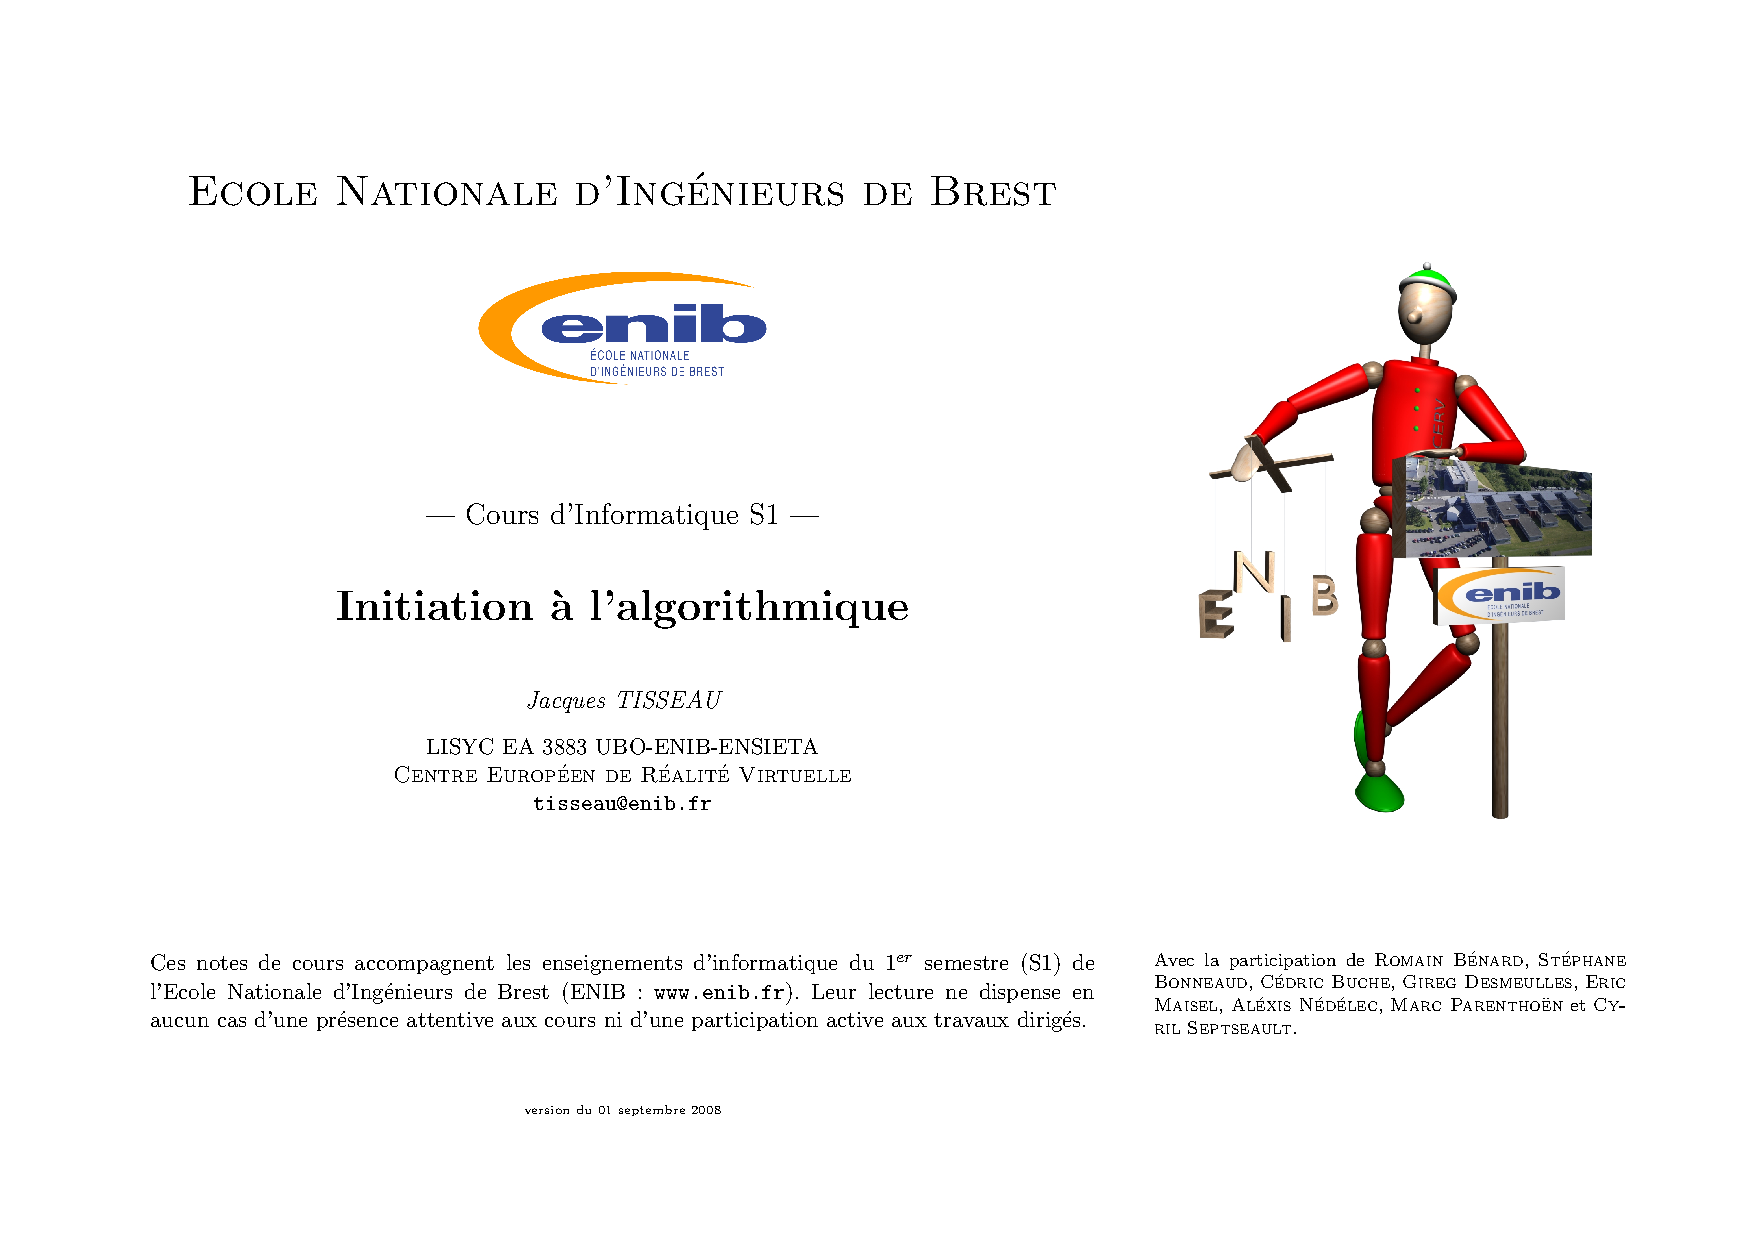
\includegraphics[width=0.9\textwidth,page=1]{../cours/info-S1.pdf}}$$
\centerline{\footnotesize
{\bf Tisseau J.},{\em Initiation à l'algorithmique}, ENIB, cours d'Informatique S1, Brest, 2009.
}
\null\vfill

\centerline{\tiny version du \today}
\end{titlepage}
%-------------------------------------------------------------------------


%-------------------------------------------------------------------------
\renewcommand{\contentsname}{Sommaire}
\tableofcontents
%-------------------------------------------------------------------------

%-------------------------------------------------------------------------
\chapter{Introduction générale}\label{ch:introduction}
%-------------------------------------------------------------------------
	% info-S1-intro.tex

\begin{td}[Dessins sur la plage : exécution (1)]\label{td:plage1}
On cherche à faire dessiner une figure géométrique sur la plage 
à quelqu'un qui a les yeux bandés.

Quelle figure géométrique dessine-t-on en exécutant la suite d'instructions 
ci-dessous ?
\begin{enumerate}
\item avance de 10 pas,
\item tourne à gauche d'un angle de $120^\circ$,
\item avance de 10 pas,
\item tourne à gauche d'un angle de $120^\circ$, 
\item avance de 10 pas.
\end{enumerate}
\end{td}

\begin{td}[Dessins sur la plage : conception (1)]\label{td:plage2}
Faire dessiner une spirale rectangulaire de 5 côtés, le plus petit côté
faisant 2 pas de long et chaque côté fait un pas de plus que le précédent.
\end{td}


\begin{td}[Propriétés d'un algorithme]\label{td:propPlage}
Reprendre le TD \ref{td:plage1} et illustrer la validité, la robustesse, la réutilisabilité, la
complexité et l'efficacité de l'algorithme proposé pour dessiner sur la plage.
\end{td}


\begin{td}[Unités d'information]\label{td:octets}\index[td]{unités d'information}
Combien y a-t-il d'octets dans 1 ko (kilooctet), 
1 Go (gigaoctet), 1 To (téraoctet), 1 Po (pétaoctet), 1 Eo (exaoctet),
1 Zo (zettaoctet) et 1 Yo (yottaoctet) ?
\end{td}

\begin{td}[Première utilisation de {\sc Python}]\label{td:python}\index[td]{{{\sc Python}}}
Se connecter sur un poste de travail d'une salle informatique.
\begin{enumerate}
\item Lancer {\sc Python}.
\item Utiliser {\sc Python} comme une simple calculette.
\item Quitter {\sc Python}.
\end{enumerate}
Ne pas oublier de se déconnecter du poste de travail.
\end{td}


	\begin{td}[Erreur de syntaxe en {\sc Python}]\label{td:erreur}\index[td]{{{\sc Python}}}
	On considère la session {\sc Python} suivante :\\[1mm]
	\mbox{}\hfill\begin{minipage}{7cm}\tt
	>>> x = 3\\
        >>> \ y = x\\
        \mbox{}\ \ File "<stdin>", line 1\\
        \mbox{}\ \ \ \ y = x\\
        \mbox{}\ \ \ \ \char`^\\
        SyntaxError: invalid syntax\\
        >>>
	\end{minipage}\\[1mm]
	De quelle erreur de syntaxe s'agit-il ?
	\end{td}
	
	\begin{td}[Dessins sur la plage : persévérance]\label{td:plage5}\index[td]{dessins sur la plage}
	Finir l'algorithme suivant qui cherche à dessiner un losange sur la plage.
	\begin{enumerate}
	\item avance de 10 pas,
	\item tourne à gauche d'un angle de $60^\circ$,
	\end{enumerate}
	\hspace*{0.9cm}\vdots
	\end{td}
	
	\begin{td}[Autonomie]\label{td:autonomie}\index[td]{autonomie}
	Trouver les définitions du mot autonomie et de son contraire (de son antonyme).
	\end{td}



\begin{td}[Site {\sc Web} d'Informatique S1]\label{td:site}\index[td]{site {{\sc Web}}}
Se connecter sur le site {\sc Web} du cours d'informatique S1 de l'ENIB et
vérifier que ces notes de cours sont bien disponibles sur le site
 au format {\tt pdf}.
\end{td}


\begin{td}[Exemple de contrôle d'attention (1)]\label{td:attention1}\index[td]{contrôle d'attention}
Répondre de mémoire aux questions suivantes (ie. sans rechercher les 
solutions dans les pages précédentes).
\begin{enumerate}
\item Quels sont les 3 principaux thèmes informatiques abordés ?
\item Quelles sont les 4 principales stratégies péda\-go\-giques suivies ?
\item Quelles sont les 3 principales qualités comportementales recherchées ?
\end{enumerate}
\end{td}


	\begin{td}[Exemple de contrôle de TD]\label{td:TD}\index[td]{contrôle de TD}
	Répondre aux questions du TD \ref{td:plage5}.
	\end{td}
	
	\begin{td}[Exemple de contrôle d'autoformation (1)]\label{td:bool}\index[td]{contrôle d'autoformation}
	Etablir la table de vérité du circuit logique ci-dessous où $a$, $b$
	et $c$ sont les entrées, $s$ et $t$ les sorties.\\[2mm]
	\centerline{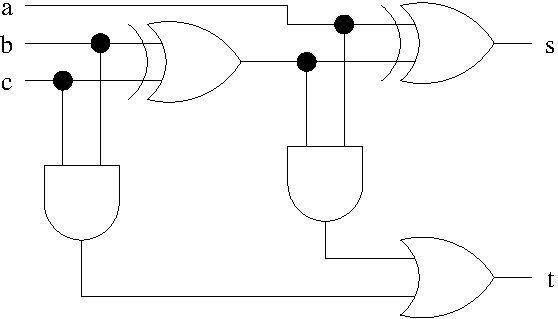
\includegraphics[width=6cm]{add3.pdf}}
	\end{td}
	
	\begin{td}[Exemple de contrôle des compétences]\label{td:competences}\index[td]{contrôle des compétences}
	Répondre aux questions du TD \ref{td:shadok} de la page \pageref{td:shadok}.
	\end{td}



\begin{td}[Nombre de contrôles]\label{td:controles}\index[td]{nombre de contrôles}
Après consultation du calendrier prévisionnel 
%de l'annexe \ref{annexe:planning} page \pageref{annexe:planning}, 
du cours d'informatique du semestre S1,
donner le nombre et le type de contrôles prévus
au calendrier du semestre.
\end{td}

	\begin{td}[Exemple de contrôle d'autoformation (2)]\label{td:negation}\index[td]{contrôle d'autoformation}
	Exprimer en la développant la négation des expressions booléennes suivantes :
	\begin{enumerate}
	\item {\tt (0 < x) and (x < 3)}
	\item {\tt (x < -2) or (x > 4)}
	\item {\tt a and (not b)}
	\item {\tt (not a) or b}
	\end{enumerate}
	\end{td}

	\begin{td}[Exemple de contrôle d'attention (2)]\label{td:attention2}\index[td]{contrôle d'attention}
	Répondre de mémoire aux questions suivantes (ie. sans rechercher les 
	solutions dans les pages précédentes).
	\begin{enumerate}
	\item Quels sont les 4 types de contrôle proposés ?
	\item Quels sont les documents que l'on peut trouver sur le site {\sc Web}
		du cours ?
	\end{enumerate}
	\end{td}

	 \begin{td}[Nombres d'exercices de TD]\label{td:exercices}\index[td]{nombres d'exercices de TD}
	 Combien d'exercices y avait-il à faire avant celui-ci ?
	 \end{td}

	\begin{td}[Environnement de travail]\label{td:labo}\index[td]{{{\sc Python}}}\index[td]{environnement de travail}
	Sur un poste de travail d'une salle informatique :
	\begin{enumerate}
	\item Quel est le type de clavier ?
	\item Comment ouvre-t-on un terminal ?
	\item Comment lance-t-on {\sc Python} ?
	\item Où sont stockés les fichiers de travail ?
	\end{enumerate}
	\end{td}

\begin{td}[QCM (1)]\label{td:qcmIntro}\index{evaluation@évaluation!contrôle d'attention}\index[td]{contrôle d'attention}
(un seul item correct par question)
\begin{enumerate}
\item L'informatique est la science
	\begin{enumerate}
	\item des dispositifs dont le fonctionnement dépend de 
		la circulation d'électrons
	\item des signaux électriques porteurs d'information ou d'énergie
	\item du traitement automatique de l'information
	\item de la commande des appareils fonctionnant sans intervention humaine
	\end{enumerate}
\item Le logiciel est
	\begin{enumerate}
	\item la mémoire de l'ordinateur
	\item le traitement automatique de l'information
	\item l'ensemble des données manipulées par les instructions
	\item un ensemble structuré d'instructions décrivant un traitement d'informations
		à faire réaliser par un matériel informatique
	\end{enumerate}
\item L'algorithmique est la science
	\begin{enumerate}
	\item du traitement automatique de l'information
	\item des algorithmes
	\item des langages de programmation
	\item des instructions
	\end{enumerate}
\item Un algorithme est
	\begin{enumerate}
	\item un ensemble de programmes remplissant une fonction déterminée,
		permettant l'accom\-plis\-se\-ment d'une tâche donnée
	\item une suite ordonnée d'instructions qui indique la démarche 
		à suivre pour résoudre une série de problèmes équivalents
	\item le nombre d'instructions élémentaires à exécuter pour
		réaliser une tâche donnée
	\item un ensemble de dispositifs physiques utilisés pour traiter
		automatiquement des informations
	\end{enumerate}
\item La validité d'un algorithme est son aptitude
	\begin{enumerate}
	\item à utiliser de manière optimale les ressources du matériel qui l'exécute
	\item à se protéger de conditions anormales d'utilisation
	\item à calculer le nombre d'instructions élémentaires nécessaires pour
		réaliser la tâche pour laquelle il a été conçu
	\item à réaliser exactement la tâche pour laquelle il a été conçu
	\end{enumerate}
\item La complexité d'un algorithme est
	\begin{enumerate}
	\item le nombre de fois où l'algorithme est utilisé dans un programme
	\item le nombre de données manipulées par les instructions de
		l'algorithme
	\item le nombre d'octets occupés en mémoire par l'algorithme
	\item le nombre d'instructions élémentaires à exécuter pour
		réaliser la tâche pour laquelle il a été conçu
	\end{enumerate}
\item Un bit est 
	\begin{enumerate}
	\item un chiffre binaire
	\item composé de 8 chiffres binaires
	\item un chiffre héxadécimal
	\item un mot d'un langage informatique
	\end{enumerate}
\item Un compilateur 
	\begin{enumerate}
	\item exécute le code source
	\item exécute le bytecode
	\item traduit un code source en code objet
	\item exécute le code objet
	\end{enumerate}
\end{enumerate}
\end{td}

\begin{td}[Puissance de calcul]\label{td:mips}\index{matériel!mips}\index[td]{puissance de calcul}
Donner l'ordre de grandeur en instructions par seconde des machines suivantes :
\begin{enumerate}
\item le premier micro-ordinateur de type PC,
\item une console de jeu actuelle,
\item un micro-ordinateur actuel,
\item {\em Deeper-Blue} : l'ordinateur qui a « battu » Kasparov aux échecs en 1997,
\item le plus puissant ordinateur actuel.
\end{enumerate}
\end{td}

\begin{td}[Stockage de données]\label{td:stock}\index[td]{stockage de données}
Donner l'ordre de grandeur en octets pour stocker en mémoire :
\begin{enumerate}
\item une page d'un livre,
\item une encyclopédie en 20 volumes,
\item une photo couleur,
\item une heure de vidéo,
\item une minute de son,
\item une heure de son.
\end{enumerate}
\end{td}

\begin{td}[Dessins sur la plage : exécution (2)]\label{td:plage3}\index[td]{dessins sur la plage}
\begin{enumerate}
\item Quelle figure géométrique dessine-t-on en exécutant la suite d'instructions 
ci-dessous ?
	\begin{enumerate}
	\item avance de 3 pas,
	\item tourne à gauche d'un angle de $90^\circ$,
	\item avance de 4 pas,
	\item rejoindre le point de départ.
	\end{enumerate}
\item Combien de pas a-t-on fait au total pour rejoindre le point de départ ?
\end{enumerate}
\end{td}

\begin{td}[Dessins sur la plage : conception (2)]\label{td:plage4}\index[td]{dessins sur la plage}
Reprendre le TD \ref{td:plage2} et illustrer la validité, la robustesse, 
la réutilisabilité, la complexité et l'efficacité de
l'algorithme proposé pour dessiner une spirale rectangulaire.
\end{td}


\begin{td}[Tracés de polygones réguliers]\label{td:tortue}\index[algo]{polygones réguliers}\index[td]{dessins sur la plage}
On cherche à faire dessiner une figure polygonale (figure \ref{fig:polygone}) 
sur la plage à quelqu'un qui a les yeux bandés.
Pour cela, on ne dispose que de 2 commandes orales :
avancer de $n$ pas en avant ($n$ est un nombre entier de pas) et 
tourner à gauche d'un angle $\theta$ (rotation sur place de $\theta$).
\begin{enumerate}
\item Faire dessiner un pentagone régulier de 10 pas de côté.
\item Faire dessiner un hexagone régulier de 10 pas de côté.
\item Faire dessiner un octogone régulier de 10 pas de côté.
\item Faire dessiner un polygone régulier de $n$ côtés de 10 pas chacun.
\end{enumerate}
\end{td}
\begin{fig}[Pentagone, hexagone, octogone]\label{fig:polygone}
\mbox{}\\
\centerline{
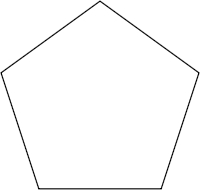
\includegraphics[width=2.5cm]{pentagone.jpg}
\hfill
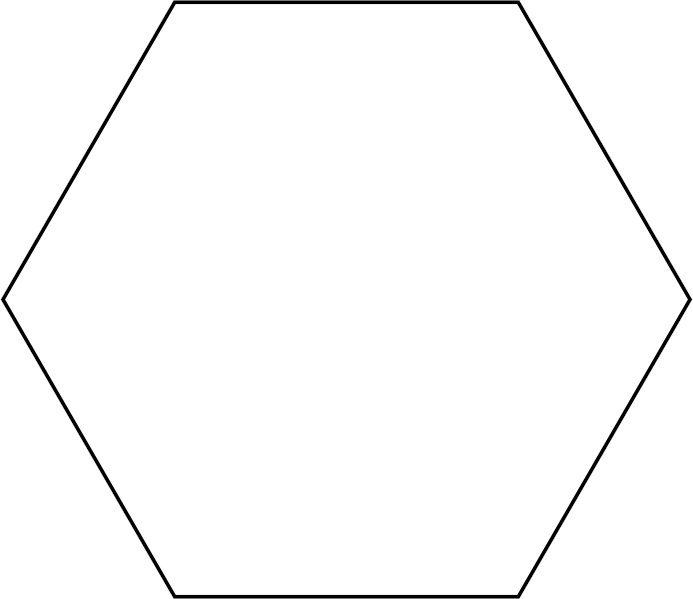
\includegraphics[width=2.5cm]{hexagone.jpg}
\hfill
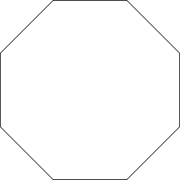
\includegraphics[width=2.5cm]{octogone.jpg}
}
\end{fig}


\begin{td}[La multiplication «~à la russe~»]\label{td:russe}\index{multiplication « à la russe »}\index[td]{multiplication « à la russe »}
La technique de multiplication dite «~à la rus\-se~» consiste à diviser par 
2 le multiplicateur (et ensuite les quotients obtenus), 
jusqu'à un quotient nul, à noter les restes,
et à multiplier parallèlement le multiplicande par 2. 
On additionne alors les multiples obtenus du multiplicande 
correspondant aux restes non nuls.

\noindent Exemple : $68 \times 123\ (= 8364)$
$$\begin{tabular}{|r|r|r|r|}
\hline
multiplicande & multiplicateur & reste      & somme partielle\\
$M \times 2$  & $m \div 2$     & $m \bmod 2$ &       \\
\hline
123  & 68 &   0   &   $(0\times 123) + 0$ \\
246  & 34 &   0   &   $(0\times 246) + 0$ \\
492  & 17 &   1   &   $(1\times 492) + 0$ \\
984  &  8 &   0   &   $(0\times 984) + 492$  \\
1968 &  4 &   0   &   $(0\times 1968) + 492$ \\
3936 &  2 &   0   &   $(0\times 3936) + 492$ \\
7872 &  1 &   1   &   $(1\times 7872) + 492$ \\
\hline
\multicolumn{3}{|r|}{$68 \times 123 =$} & 8364\\
\hline
\end{tabular}$$
\end{td}

\noindent Effectuer les multiplications suivantes selon la technique «~à la russe~».
\begin{enumerate}
\item $64 \times 96\ (= 6144)$
\item $45 \times 239\ (= 10755)$
\end{enumerate}

\begin{td}[La multiplication arabe]\label{td:ibnalbanna}
\index{multiplication arabe}\index[td]{multiplication arabe}
On consid\`ere ici le texte d'Ibn al-Banna concernant la multiplication
\`a l'aide de tableaux.

\begin{fig}[Tableau d'Ibn al-Banna]\label{fig:ibnalbanna}
\mbox{}\\
\centerline{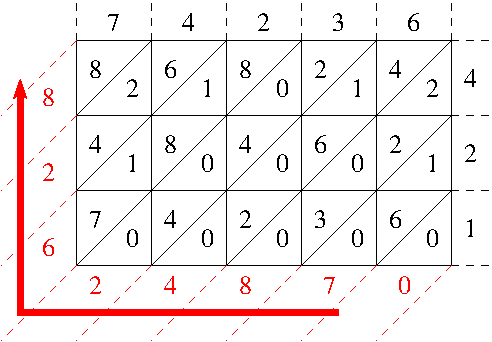
\includegraphics[width=7.5cm]{ibnalbanna.pdf}}
\end{fig}

{\footnotesize\em
« Tu construis un quadrilat\`ere que tu subdivises verticalement et
horizontalement en autant de bandes qu'il y a de positions dans les
deux nombres multipli\'es. Tu divises diagonalement les carr\'es
obtenus, \`a l'aide de diagonales allant du coin inf\'erieur gauche au
coin sup\'erieur droit (figure \ref{fig:ibnalbanna}).

Tu places le multiplicande au-dessus du quadrilat\`ere, en faisant 
correspondre chacune de ses positions \`a une colonne\footnote{L'écriture
du nombre s'effectue de droite à gauche (exemple : 352 s'écrira donc 253).}. 
Puis, tu places le multiplicateur \`a gauche ou \`a droite du quadrilat\`ere,
de telle sorte qu'il descende avec lui en faisant correspondre \'egalement 
chacune de ses positions \`a une ligne\footnote{L'écriture
du nombre s'effectue de bas en haut (exemple : {\tiny$\begin{array}{c}3\\5\\2\end{array}$} 
s'écrira donc {\tiny$\begin{array}{c}2\\5\\3\end{array}$}).}. Puis, tu multiplies, 
l'une apr\`es l'autre, chacune des positions du multiplicande du carr\'e 
par toutes les positions du multiplicateur, et tu poses le r\'esultat 
partiel correspondant \`a chaque position dans le carr\'e o\`u se coupent 
respectivement leur colonne et leur ligne, en pla\c{c}ant les unit\'es 
au-dessus de la diagonale et les dizaines en dessous. Puis, tu
commences \`a additionner, en partant du coin sup\'erieur gauche :
tu additionnes ce qui est entre les diagonales, sans effacer, 
en pla\c{c}ant chaque nombre dans sa position, en transf\'erant 
les dizaines de chaque somme partielle \`a la diagonale suivante et
en les ajoutant \`a ce qui y figure. 

La somme que tu obtiendras sera le r\'esultat. »}

\noindent En utilisant la m\'ethode du tableau d'Ibn al-Banna, calculer $63247\times124$ 
($= 7842628$).
\end{td}

\begin{td}[La division chinoise]\label{td:boulier}
\index{division chinoise}\index[td]{division chinoise}
Dans sa version actuelle, le boulier chinois se compose d'un nombre variable de tringles
serties dans un cadre rectangulaire. Sur chacune de ces tringles, deux étages de boules
séparées par une barre transversale peuvent coulisser librement (figure \ref{fig:boulier}).
La notation des nombres repose sur le principe de la numération de position : chacune
des 2 boules du haut vaut 5 unités et chacune des 5 boules du bas vaut 1 unité. Seules
comptent les boules situées dans la région transversale.

Il existe des règles spéciales de division pour chaque diviseur de 1 à 9.
On consid\`ere ici les 7 r\`egles de division par 7 (figure \ref{fig:div7}) :

\noindent\begin{minipage}[t]{7.5cm}\footnotesize
\begin{enumerate}
\item {\em «~qi-yi xia jia san~»} : 7-1 ? ajouter 3 en dessous !
\item {\em «~qi-er xia jia liu~»} : 7-2 ? ajouter 6 en dessous !
\item {\em «~qi-san si sheng er~»} : 7-3 ? 4 reste 2 !
\end{enumerate}
\end{minipage}\hfill
\begin{minipage}[t]{7.5cm}\footnotesize
\begin{enumerate}\setcounter{enumi}{3}
\item {\em «~qi-si wu sheng wu~»} : 7-4 ? 5 reste 5 !
\item {\em «~qi-wu qi sheng yi~»} : 7-5 ? 7 reste 1 !
\item {\em «~qi-liu ba sheng si~»} : 7-6 ? 8 reste 4 !
\item {\em «~feng-qi jin yi~»} : 7-7 ? 1 monté !
\end{enumerate}
\end{minipage}

\begin{fig}[Boulier chinois]\label{fig:boulier}
\mbox{}\\
\centerline{\em
8017 :
\begin{minipage}{5cm}
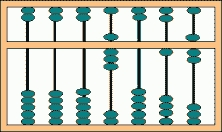
\includegraphics[width=5cm]{boulier.jpg}
\end{minipage}}
\end{fig}

\begin{fig}[Règles de la division par 7]\label{fig:div7}
\mbox{}\\
\centerline{\em\begin{tabular}[t]{|c|c|c|}
\hline
Règle & Avant & Après \\
\hline
\hline
7-1   & 
\begin{tabular}{ccccc}
1 & \makebox[0.5mm]{} & 0 & 0 & 0 \\
\hline
2 & & 0 & 1 & 0
\end{tabular} &
\begin{tabular}{ccccc}
1 & \makebox[0.5mm]{} & 0 & 0 & 0 \\
\hline
2 & & 0 & 1 & 3
\end{tabular} \\
\hline
\hline
7-2   & 
\begin{tabular}{ccccc}
1 & \makebox[0.5mm]{} & 0 & 0 & 0 \\
\hline
2 & & 0 & 2 & 0
\end{tabular} &
\begin{tabular}{ccccc}
1 & \makebox[0.5mm]{} & 0 & 0 & 1 \\
\hline
2 & & 0 & 2 & 1
\end{tabular} \\
\hline
\hline
7-3   & 
\begin{tabular}{ccccc}
1 & \makebox[0.5mm]{} & 0 & 0 & 0 \\
\hline
2 & & 0 & 3 & 0
\end{tabular} &
\begin{tabular}{ccccc}
1 & \makebox[0.5mm]{} & 0 & 0 & 0 \\
\hline
2 & & 0 & 4 & 2
\end{tabular} \\
\hline
\hline
7-4   & 
\begin{tabular}{ccccc}
1 & \makebox[0.5mm]{} & 0 & 0 & 0 \\
\hline
2 & & 0 & 4 & 0
\end{tabular} &
\begin{tabular}{ccccc}
1 & \makebox[0.5mm]{} & 0 & 1 & 1 \\
\hline
2 & & 0 & 0 & 0
\end{tabular} \\
\hline
\end{tabular}
\hspace*{2mm}
\begin{tabular}[t]{|c|c|c|}
\hline
Règle & Avant & Après \\
\hline
\hline
7-5   & 
\begin{tabular}{ccccc}
1 & \makebox[0.5mm]{} & 0 & 1 & 0 \\
\hline
2 & & 0 & 0 & 0
\end{tabular} &
\begin{tabular}{ccccc}
1 & \makebox[0.5mm]{} & 0 & 1 & 0 \\
\hline
2 & & 0 & 2 & 1
\end{tabular} \\
\hline
\hline
7-6   & 
\begin{tabular}{ccccc}
1 & \makebox[0.5mm]{} & 0 & 1 & 0 \\
\hline
2 & & 0 & 1 & 0
\end{tabular} &
\begin{tabular}{ccccc}
1 & \makebox[0.5mm]{} & 0 & 1 & 0 \\
\hline
2 & & 0 & 3 & 4
\end{tabular} \\
\hline
\hline
7-7   & 
\begin{tabular}{ccccc}
1 & \makebox[0.5mm]{} & 0 & 1 & 0 \\
\hline
2 & & 0 & 2 & 0
\end{tabular} &
\begin{tabular}{ccccc}
1 & \makebox[0.5mm]{} & 0 & 0 & 0 \\
\hline
2 & & 1 & 0 & 0
\end{tabular} \\
\hline
\end{tabular}}
\end{fig}
Ces règles ne sont pas des règles logiques, 
mais de simples procédés mnémotechniques
indiquant ce qu'il convient de faire selon la situation. Leur énoncé débute par le
rappel du diviseur, ici 7, et se poursuit par l'énoncé du dividende, par exemple 3 :
7-3. Le reste de la règle indique quelles manipulations effectuées, ajouts ou retraits
de boules. Il faut également savoir que le dividende étant posé sur le boulier, on doit
appliquer les règles aux chiffres successifs du dividende, en commençant par celui dont
l'ordre est le plus élevé.
«~ajouter en dessous~» veut dire «~mettre des boules au rang 
immédiatement inférieur (à droite) au rang considéré~» et «~monter~» veut dire «~mettre des boules
au rang immédiatement supérieur (à gauche) au rang considéré~».


Pour effectuer la division d'un nombre par 7, on pose le dividende à droite sur le
boulier et le diviseur (7) à gauche. On opère sur les chiffres successifs du dividende
en commençant par celui d'ordre le plus élevé (le plus à gauche). Les règles
précédemment énoncées sont appliquées systématiquement.

Utiliser un boulier chinois pour diviser 1234 par 7 ($1234 = 176\times 7 + 2$).

\centerline{\begin{tabular}{cccccc}
1 & \makebox[1mm]{} & 0 & 0 & 0 & 0 \\
\hline
2 & & 1 & 2 & 3 & 4
\end{tabular}
$\rightarrow$
\begin{tabular}{cccccc}
1 & \makebox[1mm]{} & 0 & 1 & 1 & 0 \\
\hline
2 & & 1 & 2 & 1 & 2
\end{tabular}}
\end{td}

\begin{td}[Le calcul Shadok]\label{td:shadok}\index{calcul {{\sc Shadok}}}\index[td]{calcul {{\sc Shadok}}}
Les cerveaux des Shadoks avaient une capacité tout à fait limitée.
Ils ne comportaient en tout que 4 cases.
Comme ils n'avaient que 4 cases, évidemment les Shadoks ne connaissaient 
pas plus de 4 mots :  {\sc ga, bu, zo et meu} (figure \ref{fig:bdShadok}).
\begin{fig}[Les Shadoks : {\sc ga} {\sc bu} {\sc zo} {\sc meu}]\label{fig:bdShadok}
\mbox{}\\
\centerline{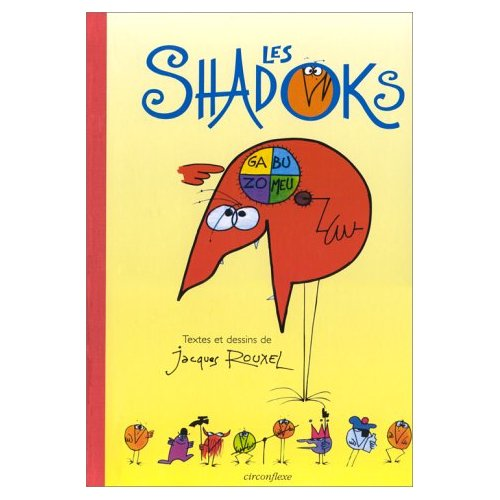
\includegraphics[width=7cm]{bdShadok.jpg}}
\end{fig}
Etant donné qu'avec 4 mots, ils ne pouvaient pas compter plus loin que 4,
le Professeur Shadoko avait réformé tout ça :
\begin{itemize}
\item Quand il n'y a pas de Shadok, on dit {\sc ga} et on écrit {\sc ga}.
\item Quand il y a un Shadok de plus, on dit {\sc bu} et on écrit {\sc bu}.
\item Quand il y a encore un Shadok, on dit {\sc zo} et on écrit {\sc zo}.
\item Et quand il y en a encore un autre, on dit {\sc meu} et on écrit {\sc meu}.
\end{itemize}

Tout le monde applaudissait très fort et trouvait ça génial sauf le Devin Plombier 
qui disait qu'on n'avait pas idée d'inculquer à des enfants des bêtises pareilles 
et que Shadoko, il fallait le condamner. 
Il fut très applaudi aussi. Les mathématiques, 
cela les intéressait, bien sûr, mais brûler le professeur, c'était intéressant aussi, faut dire. 
Il fut décidé à l'unanimité qu'on le laisserait parler et qu'on le brûlerait après, à la récréation.
\begin{itemize}
\item Répétez avec moi : {\sc meu} {\sc zo} {\sc bu} {\sc ga}\ldots {\sc ga} {\sc bu} {\sc zo} {\sc meu}.
\item Et après! ricanait le Plombier.
\item Si je mets un Shadok en plus, évidemment, je n'ai plus assez 
de mots pour les compter, alors c'est très simple : on les jette dans une poubelle, 
et je dis que j'ai {\sc bu} poubelle. Et pour ne pas confondre avec le {\sc bu} du début, 
je dis qu'il n'y a pas de Shadok à côté de la poubelle et j'écris {\sc bu} {\sc ga}. 
{\sc bu} Shadok à côté de la poubelle: {\sc bu} {\sc bu}. Un autre : {\sc bu} {\sc zo}. Encore un autre : {\sc bu} {\sc meu}. 
On continue. {\sc zo} poubelles et pas de Shadok à côté : {\sc zo} {\sc ga}\ldots 
{\sc meu} poubelles et {\sc meu} Shadoks à côté : {\sc meu} {\sc meu}. 
Arrivé là, si je mets un Shadok en plus, il me faut une autre poubelle. 
Mais comme je n'ai plus de mots pour compter les poubelles, je m'en débarrasse 
en les jetant dans une grande poubelle. 
J'écris {\sc bu} grande poubelle avec pas de petite poubelle 
et pas de Shadok à côté: {\sc bu} {\sc ga} {\sc ga}, et on continue\ldots {\sc bu} {\sc ga} {\sc bu}, 
{\sc bu} {\sc ga} {\sc zo}\ldots {\sc meu} {\sc meu} {\sc zo}, {\sc meu} {\sc meu} {\sc meu}.
Quand on arrive là et qu'on a trop de grandes poubelles pour pouvoir les compter, 
eh bien, on les met dans une super-poubelle, on écrit {\sc bu} {\sc ga} {\sc ga} {\sc ga}, 
et on continue\ldots (figure \ref{fig:calculShadok}).
\end{itemize}
\begin{fig}[Les 18 premiers nombres Shadok]\label{fig:calculShadok}
$$\begin{tabular}[t]{l@{ : }ll@{ : }ll@{ : }l}
0 & {\sc ga} 	      & 6  & {\sc bu} {\sc zo}  & 12 & {\sc meu} {\sc ga}\\
1 & {\sc bu} 	      & 7  & {\sc bu} {\sc meu} & 13 & {\sc meu} {\sc bu}\\
2 & {\sc zo} 	      & 8  & {\sc zo} {\sc ga}  & 14 & {\sc meu} {\sc zo}\\
3 & {\sc meu} 	      & 9  & {\sc zo} {\sc bu}  & 15 & {\sc meu} {\sc meu}\\
4 & {\sc bu} {\sc ga} & 10 & {\sc zo} {\sc zo}  & 16 & {\sc bu} {\sc ga} {\sc ga}\\
5 & {\sc bu} {\sc bu} & 11 & {\sc zo} {\sc meu} & 17 & {\sc bu} {\sc ga} {\sc bu}
\end{tabular}$$
\end{fig}

\noindent\begin{enumerate}
\item Quels sont les entiers décimaux représentés en «~base Shadok~» 
	par les expressions suivantes ?
	\begin{enumerate}
	\item {\sc ga} {\sc ga}
	\item {\sc bu} {\sc bu} {\sc bu}
	\item {\sc zo} {\sc zo} {\sc zo} {\sc zo}
	\item {\sc meu} {\sc meu} {\sc meu} {\sc meu} {\sc meu} 
	\end{enumerate}	
\item Effectuer les calculs Shadok suivants.
	\begin{enumerate}
	\item {\sc zo} {\sc zo} {\sc meu} $+$ {\sc bu} {\sc ga} {\sc meu}
	\item {\sc meu} {\sc ga} {\sc meu} $-$ {\sc bu} {\sc meu} {\sc ga}
	\item {\sc zo} {\sc meu} {\sc meu} $\times$ {\sc bu} {\sc ga} {\sc meu}
	\item {\sc zo} {\sc zo} {\sc zo} {\sc meu} $\div$ {\sc bu} {\sc ga} {\sc zo}
	\end{enumerate}
\end{enumerate}
\end{td}




%-------------------------------------------------------------------------
\chapter{Instructions de base}\label{ch:instructions}
%-------------------------------------------------------------------------
	%-------------------------------------------------------------------------
% td-info-S1-instructions.tex
%-------------------------------------------------------------------------

\begin{td}[Unité de pression]\label{td:torr}\index[td]{unité de pression}
\em
Le torr (torr) ou millimètre de mercure (mmHg) est une unité de mesure 
de la pression qui tire son nom du physicien et mathématicien italien Evangelista Torricelli (1608-1647).
Il est défini comme la pression exercée à 0°C par une colonne de 1 millimètre de mercure (mmHg).
Il a plus tard été indexée sur la pression atmosphérique : 1 atmosphère normale correspond à 
760 mmHg et a 101 325 Pa.

Ecrire une instruction qui permette de passer directement des torrs au pascals (Pa).
\end{td}

	\begin{td}[Suite arithmétique (1)]\label{td:suiteArit}\index[td]{suite arithmétique}
\em
	Ecrire une instruction qui calcule la somme $s = \sum_0^n u_k$ des $n$ premiers 
	termes d'une suite arithmétique $u_k = a + r\cdot k$. 
	\end{td}

\begin{td}[Permutation circulaire (1)]\label{td:permutation1}\index[td]{permutation circulaire}
\em
Effectuer une permutation circulaire droite entre les valeurs de 4 entiers $x$, $y$, $z$ et $t$.
\end{td}

\begin{td}[Séquence d'affectations (1)]\label{td:seq1}\index[td]{séquence d'affectations}
\em
Quelles sont les valeurs des variables $a$, $b$, $q$ et $r$ 
après la séquence d'affectations suivante ?
	
	\noindent{\footnotesize\tt
	\mbox{}\ \ a = 19\\
	\mbox{}\ \ b = 6\\
	\mbox{}\ \ q = 0\\
	\mbox{}\ \ r = a\\
	\mbox{}\ \ r = r - b\\
	\mbox{}\ \ q = q + 1\\
	\mbox{}\ \ r = r - b\\
	\mbox{}\ \ q = q + 1\\
	\mbox{}\ \ r = r - b\\
	\mbox{}\ \ q = q + 1
	}
\end{td}

\begin{td}[Opérateurs booléens dérivés (1)]\label{td:booleens1}\index[td]{opérateurs booléens dérivés}
\em
En utilisant les opérateurs booléens de base ({\tt not}, {\tt and} et {\tt or}),
ecrire un algorithme qui affecte successivement à une variable {\tt s} 
le résultat des opérations booléennes suivantes :
ou exclusif ({\em xor}, $a \oplus b$), 
non ou ({\em nor}, $\overline{a+b}$), 
non et ({\em nand}, $\overline{a\cdot b}$), 
implication ($a \Rightarrow b$) et  
équivalence ($a \Leftrightarrow b$).
\end{td}

\index[algo]{circuits logiques}
\begin{td}[Circuit logique (1)]\label{td:circuits}\index[td]{circuits logiques}
\em
Donner les séquences d'affectations permettant de calculer la sortie $s$
du circuit logique suivant en fonction de ses entrées $a$, $b$ et $c$.
$$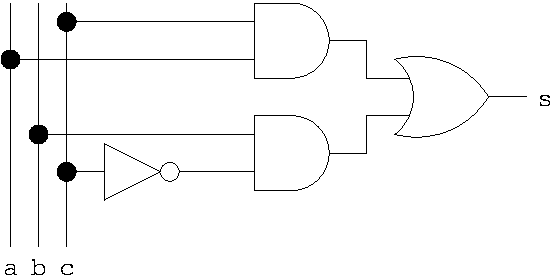
\includegraphics[width=5cm]{mux1.pdf}$$
\end{td}

\begin{td}[Lois de De Morgan]\label{td:prop}\index{{{\sc De Morgan}}}\index[td]{lois de {{\sc De Morgan}}}
\em
Démontrer à l'aide des tables de vérité les lois de De Morgan 
$\forall a, b \in \{0;1\}$ :
\begin{enumerate}
\item {$\overline{(a+b)} = \overline{a} \cdot \overline{b}$} 
\item {$\overline{(a \cdot b)} = \overline{a} + \overline{b}$}
\end{enumerate}
\end{td}


\begin{td}[Maximum de 2 nombres]\label{td:max}\index[algo]{maximum de 2 nombres}\index[td]{maximum de 2 nombres}
\em
Ecrire un algorithme qui détermine le maximum $m$ de 2 nombres $x$ et $y$.
\end{td}

\begin{td}[Fonction « porte »]\label{td:porte}\index[td]{fonction porte}
\em
Proposer une autre alternative simple pour calculer la fonction « porte » de
l'exemple ci-dessous.\\
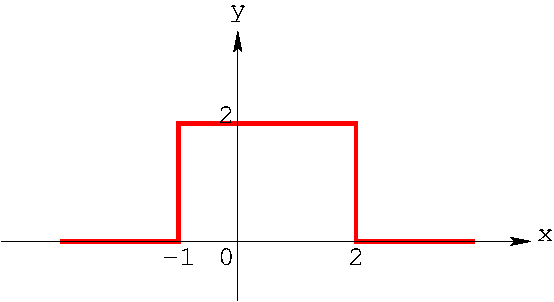
\includegraphics[width=3cm]{porte.pdf}
\end{td}

\begin{td}[Ouverture d'un guichet]\label{td:guichet}\index[td]{ouverture d'un guichet}
\em
A l'aide d'alternatives simples imbriquées, écrire un algorithme qui détermine 
si un guichet est {\tt 'ouvert'} ou 
{\tt 'fermé'} selon les jours de la semaine ({\tt 'lundi'}, {\tt 'mardi'},
\ldots\ ,{\tt 'dimanche'}) et l'heure de la journée (entre 0h et 24h).
Le guichet est ouvert tous les jours de 8h à 13h et de 14h à 17h 
sauf le samedi après-midi et toute la journée du dimanche.
\end{td}

\begin{td}[Catégorie sportive]\label{td:categorie}\index[td]{catégorie sportive}
\em
Ecrire un algorithme qui détermine la catégorie sportive d'un enfant selon
son âge : 
	\begin{itemize}
	\item Poussin de 6 à 7 ans,
	\item Pupille de 8 à 9 ans,
	\item Minime de 10 à 11 ans,
	\item Cadet de 12 ans à 14 ans.
	\end{itemize}
\end{td}

\begin{td}[Dessin d'étoiles (1)]\label{td:etoile}\index[td]{dessin d'étoiles}
\em
Ecrire un algorithme itératif qui affiche les $n$ lignes suivantes (l'exemple
est donné ici pour $n=6$) : \\
\begin{minipage}[t]{2cm}\tt
******\\
*****\\
****\\
***\\
**\\
*
\end{minipage}
\hfill
\begin{minipage}[t]{3cm}
Rappel \python\ : \\
{\tt
\mbox{}\ \ \ \ >>> 5*'r'\\
\mbox{}\ \ \ \ 'rrrrr'\\
\mbox{}\ \ \ \ >>> 2*'to'\\
\mbox{}\ \ \ \ 'toto'
}
\end{minipage}
\end{td}

\begin{td}[Fonction factorielle]\label{td:factorielle}\index[algo]{fonction factorielle}\index[td]{fonction factorielle}
\em
Ecrire un algorithme qui calcule $n! = 1\cdot 2\cdot 3\cdot \ldots \cdot (n-1)\cdot n$.
\end{td}

\begin{td}[Fonction sinus]\label{td:sinus}\index[algo]{développements limités}\index[td]{fonction sinus}
\em
Ecrire un algorithme qui calcule de manière itérative la fonction sinus
en fonction de son d\'eveloppement en série entière.\\
$$\displaystyle\sin(x) \approx \sum_{k=0}^{n} u_k = \sum_{k=0}^{n} (-1)^k\frac{x^{2k+1}}{(2k+1)!} = x - \frac{x^3}{6} + \frac{x^5}{120} + \ldots + (-1)^n\frac{x^{2n+1}}{(2n+1)!}$$
Les calculs seront arr\^et\'es lorsque la valeur absolue du terme $u_k$ sera 
inf\'erieure \`a un certain seuil $s$ ($0 < s < 1$). On n'utilisera ni la fonction 
{\em puissance} ($x^n$) ni la fonction {\em facto\-riel\-le} ($n!$) pour effectuer
le calcul de $\sin(x)$.
\end{td}

\begin{td}[Algorithme d'Euclide]\label{td:euclide}\index[td]{algorithme d'{{\sc Euclide}}}
\em
Dans la tradition grecque, en comprenant un nombre entier comme une longueur, 
un couple d'entiers comme un rectangle, leur pgcd est la taille du plus grand 
carré permettant de carreler ce rectangle. L'algorithme décompose ce rectangle 
en carrés, de plus en plus petits, par divisions euclidiennes successives, 
de la longueur par la largeur, puis de la largeur par le reste, 
jusqu'à un reste nul.\\
Faire la construction géométrique «~à la grecque antique~» qui permet de déterminer 
le pgcd $d$ de $a=21$ et $b=15$ ($d=3$).
\end{td}

\begin{td}[Division entière]\label{td:division}\index[td]{division entière}
\em
Ecrire un algorithme itératif qui calcule le quotient $q$ et le reste $r$ de la 
division entière $a\div b$ ($a = bq+r$).\\
On n'utilisera pas les opérateurs prédéfinis {\tt /} et {\tt \%} mais
on pourra s'inspirer du TD \ref{td:seq1} page \pageref{td:seq1}.
\end{td}


\begin{td}[Affichage inverse]\label{td:caractere}\index[td]{affichage inverse}
\em
Ecrire un algorithme qui affiche les caractères d'une chaîne {\tt s},
un par ligne en partant de la fin de la chaîne.
\end{td}

\begin{td}[Parcours inverse]\label{td:parcours}\index[td]{parcours inverse}
\em
Ecrire un algorithme qui parcourt en sens inverse une séquence {\tt s}
quelconque (du dernier élément au premier élément).
\end{td}
%\begin{fig}[Boucle {\tt for}]\label{fig:for}
%\tt for element in s : blocFor\\
%\centerline{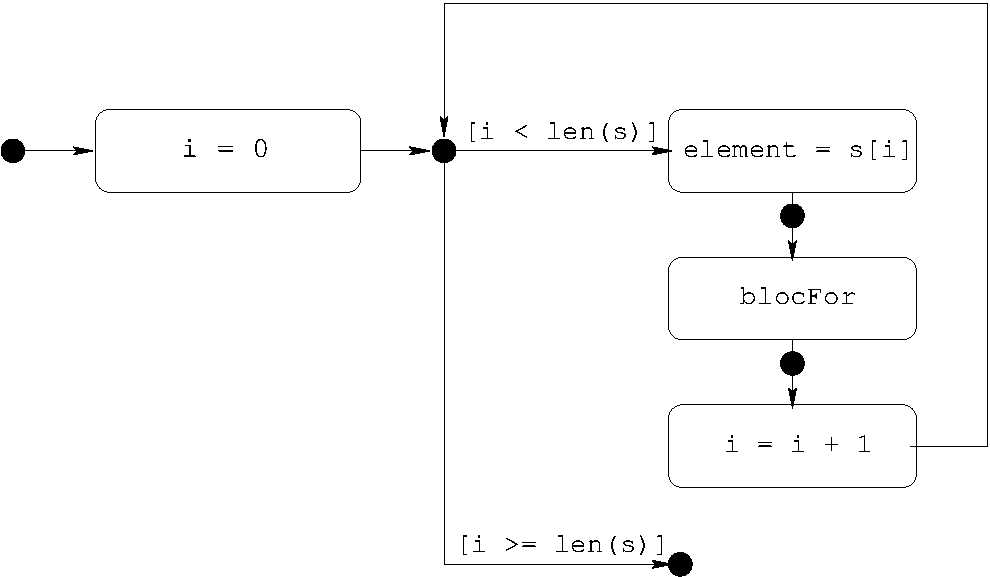
\includegraphics[width=7.5cm]{uml7.pdf}}
%\end{fig}

\begin{td}[Suite arithmétique (2)]\label{td:suiteArit2}\index[algo]{suites numériques}
\em
\begin{enumerate}
\item Ecrire un algorithme qui calcule de manière itérative la somme $s = \sum_0^n u_k$ des $n$ premiers 
	termes d'une suite arithmétique $u_k = a + r\cdot k$. On utilisera une boucle {\tt for}.
\item Comparer l'efficacité de cette approche itérative avec le calcul du TD \ref{td:suiteArit} 
	page \pageref{td:suiteArit}.
\end{enumerate}
\end{td}


\begin{td}[Dessin d'étoiles (2)]\label{td:etoile2}\index[td]{dessin d'étoiles}
\em
Reprendre le TD \ref{td:etoile} page \pageref{td:etoile} en supposant qu'on ne peut 
afficher qu'une étoile à la fois (on s'interdit ici la possibilité d'écrire
{\tt 5*'*'} à la place de {\tt '*****'} par exemple).
\end{td}

\begin{td}[Opérateurs booléens dérivés (2)]\label{td:booleens2}\index[td]{opérateurs booléens dérivés}
\em
A l'aide d'itérations imbriquées, afficher les tables de vérité des 
opérateurs logiques dérivés (voir TD \ref{td:booleens1}) : 
ou exclusif ({\em xor}, $a \oplus b$), 
non ou ({\em nor}, $\overline{a+b}$), 
non et ({\em nand}, $\overline{a\cdot b}$), 
implication ($a \Rightarrow b$) et  
équivalence ($a \Leftrightarrow b$).
\end{td}

\begin{td}[Damier]\label{td:damier}\index[td]{damier}
\em
En utilisant les instructions {\em à la {\sc Logo}} de l'annexe \ref{logo} page \pageref{logo},
dessiner un damier rectangulaire de $n\times m$ cases.
\end{td}

\begin{td}[Trace de la fonction factorielle]\label{td:traceFactorielle}\index[td]{fonction factorielle}
\em
Tracer la fonction factorielle du TD \ref{td:factorielle} page
\pageref{td:factorielle}.
\end{td}

\begin{td}[Figure géométrique]\label{td:quinconce}\index[td]{figure géométrique}
\em
Que dessinent les instructions suivan\-tes ?
\vspace*{1mm}

	{\tt \mbox{}\ \ }\begin{minipage}{5cm}\tt
	x0 = 0\\
	y0 = 0\\
	r = 10\\
	n = 5\\
	m = 10\\
	for i in range(n) :\\
	\mbox{}\ \ \ \ up()\\
	\mbox{}\ \ \ \ y = y0 - 2*r*i\\
	\mbox{}\ \ \ \ x = x0 + r*(i\%2)\\
	\mbox{}\ \ \ \ goto(x,y)\\
	\mbox{}\ \ \ \ for j in range(m) :\\
	\mbox{}\ \ \ \ \ \ \ \ down()\\
	\mbox{}\ \ \ \ \ \ \ \ circle(r)\\
	\mbox{}\ \ \ \ \ \ \ \ up()\\
	\mbox{}\ \ \ \ \ \ \ \ x = x + 2*r\\
	\mbox{}\ \ \ \ \ \ \ \ goto(x,y)
	\end{minipage}
\end{td}

\begin{td}[Suite arithmétique (3)]\label{td:suiteArit3}
Reprendre le TD \ref{td:suiteArit2} page \pageref{td:suiteArit2} en explicitant l'invariant, la condition d'arrêt,
la progression et l'initialisation de la boucle retenue.
\end{td}

\begin{td}[QCM (2)]\label{td:qcmInstruc}\index{evaluation@évaluation!contrôle d'attention}\index[td]{contrôle d'attention}(un seul item correct par question)
\em
\begin{enumerate}
\item En {\sc Python}, l'instruction « ne rien faire » se dit
	\begin{enumerate}
	\item {\tt break}
	\item {\tt return}
	\item {\tt pass}
	\item {\tt continue}
	\end{enumerate}
\item Une variable informatique est un objet 
	\begin{enumerate}
	\item équivalent à une variable mathématique
	\item qui associe un nom à une valeur
	\item qui varie nécessairement
	\item qui modifie la mémoire
	\end{enumerate}
\item L'affectation consiste à
	\begin{enumerate}
	\item comparer la valeur d'une variable à une autre valeur
	\item associer une valeur à une variable
	\item incrémenter une variable
	\item déplacer une variable en mémoire
	\end{enumerate}
\item Après la séquence \fbox{\footnotesize\tt\begin{tabular}{l}a = 13\\b = 4\\b = a\\a = b\end{tabular}} les variables {\tt a} et {\tt b} sont telles que
	\begin{enumerate}
	\item {\tt a = 13} et {\tt b = 13}
	\item {\tt a = 4} et {\tt b = 4}
	\item {\tt a = 4} et {\tt b = 13}
	\item {\tt a = 13} et {\tt b = 4}
	\end{enumerate}
\item Le résultat d'une comparaison est une valeur
	\begin{enumerate}
	\item réelle
	\item qui dépend du type des arguments 
	\item booléenne
	\item entière
	\end{enumerate}
\item Un opérateur booléen s'applique à des valeurs
	\begin{enumerate}
	\item booléennes
	\item entières
	\item réelles
	\item alphanumériques
	\end{enumerate}
\item La fonction principale d'une instruction de test est
	\begin{enumerate}
	\item de passer d'instruction en instruction
	\item de répéter une instruction sous condition
	\item d'exécuter une instruction sous condition
	\item d'interrompre l'exécution d'une instruction
	\end{enumerate}
\item Après la séquence \fbox{\footnotesize\tt\begin{tabular}{l}x = -3\\if   x < -4 : y = 0\\elif x < -3 : y = 4 - x\\elif x < -1 : y = x*x + 6*x + 8\\elif x < 3 : y = 2 - x\\else : y = -2\end{tabular}} la variable {\tt y} est telle que
	\begin{enumerate}
	\item {\tt y = -1}
	\item {\tt y = 0}
	\item {\tt y = 7}
	\item {\tt y = -2}
	\end{enumerate}
\item L'itération conditionnelle est une instruction de contrôle du flux d'instructions 
	\begin{enumerate}
	\item qui permet d'exécuter une instruction sous condition préalable.
	\item qui est vérifiée tout au long de son exécution. 
	\item qui permet sous condition préalable de répéter zéro ou plusieurs fois la même instruction.
	\item qui permet de choisir entre plusieurs instructions.
	\end{enumerate}
\item On ne sort jamais d'une boucle si la condition d'arrêt 
	\begin{enumerate}
	\item ne varie pas en cours d'exécution.
	\item ne contient pas d'opérateurs booléens.
	\item est toujours fausse.
	\item n'est jamais fausse.
	\end{enumerate}
\item Que vaut {\tt f} à la fin des instructions suivantes si $n = 5$ ?

	\begin{py}{4cm}
	\begin{verbatim}
	f = 0
	i = 1
	while i < n+1:
	    f = f + i
	    i = i + 1
	\end{verbatim}
	\end{py}

	\begin{enumerate}
	\item 6
	\item 10
	\item 15
	\item 21
	\end{enumerate}
\item Une séquence est une suite ordonnée 
	\begin{enumerate}
	\item d'éléments que l'on peut référencer par leur rang.
	\item d'instructions formant un ensemble logique.
	\item d'instructions conditionnelles.
	\item de nombres
	\end{enumerate}
\item Dans la chaîne {\tt s = 'gérard'}, {\tt s[2]} vaut
	\begin{enumerate}
	\item {\tt 'é'}
	\item {\tt 'r'}
	\item {\tt 'gé'}
	\item {\tt 'gér'}
	\end{enumerate}
\item Que vaut {\tt f} à la fin des instructions suivantes si $n = 5$ ?

	\begin{py}{4cm}
	\begin{verbatim}
	f = 1
	for i in range(2,n+1) :
	    f = f * i
	\end{verbatim}
	\end{py}

	\begin{enumerate}
	\item 120
	\item 720
	\item 6
	\item 24
	\end{enumerate}
\item Que vaut {\tt f} à la fin des instructions suivantes si $n = 5$ ?

	\begin{py}{4cm}
	\begin{verbatim}
	f, f1, f2 = 2,1,1
	for i in range(3,n+1) :
	    f2 = f1
	    f1 = f
	    f = f1 + f2
	\end{verbatim}
	\end{py}

	\begin{enumerate}
	\item 3
	\item 5
	\item 8
	\item 13
	\end{enumerate}
\end{enumerate}
\end{td}


\begin{td}[Unité de longueur]\label{td:al}\em \index[td]{unité de longueur}
L'année-lumière (al) est une unité de distance utilisée en astronomie. 
Une année-lumière est la distance parcourue par un photon (ou plus simplement la lumière) 
dans le vide, en dehors de tout champ gravitationnel ou magnétique, en une année julienne 
(365,25 jours). 

Ecrire une instruction qui permette de passer directement des années-lumière aux m/s sachant que
la vitesse de la lumière dans le vide est de 299 792 458 m/s.
\end{td}

\begin{td}[Permutation circulaire (2)]\label{td:permutation2}\em \index[algo]{permutation circulaire}\index[td]{permutation circulaire}
 Effectuer une permutation circulaire gauche entre les valeurs de 3 entiers $x$, $y$ et $z$.
\end{td}

\begin{td}[Séquence d'affectations (2)]\label{td:seq2}\em \index[td]{séquence d'affectations}
	Quelles sont les valeurs des variables $n$ et $s$
	après la séquence d'affectations suivante ?
	
	\noindent{\footnotesize\tt
	\mbox{}\ \ n = 1\\
	\mbox{}\ \ s = n\\
	\mbox{}\ \ n = n + 1\\
	\mbox{}\ \ s = s + n\\
	\mbox{}\ \ n = n + 1\\
	\mbox{}\ \ s = s + n\\
	\mbox{}\ \ n = n + 1\\
	\mbox{}\ \ s = s + n\\
	\mbox{}\ \ n = n + 1\\
	\mbox{}\ \ s = s + n
	}
\end{td}

\begin{td}[Circuits logiques (2)]\label{td:circuits2}\em \index[algo]{circuits logiques}\index[td]{circuits logiques}
On considère les conventions graphiques traditionnelles pour les opérateurs logiques :
$$\begin{tabular}{ccccccc}
$\overline{a}$ & $a \cdot b$ & $a + b$ & $a \oplus b$ & $a \cdot b \cdot c$ & $a + b + c$ & $\overline{a \cdot b \cdot c}$ \\
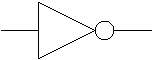
\includegraphics[height=1cm]{non.pdf} & 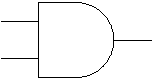
\includegraphics[height=1cm]{et.pdf} & 
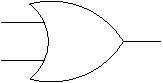
\includegraphics[height=1cm]{ou.pdf}  & 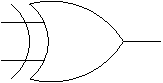
\includegraphics[height=1cm]{xor.pdf} & 
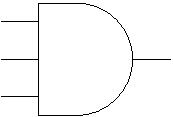
\includegraphics[height=1cm]{et3.pdf} & 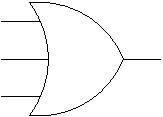
\includegraphics[height=1cm]{ou3.pdf} & 
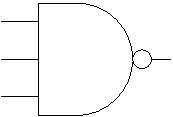
\includegraphics[height=1cm]{nonet3.pdf}
\end{tabular}$$
Donner les séquences d'affectations permettant de calculer la (ou les) sortie(s)
des circuits logiques suivants en fonction de leurs entrées.

\begin{minipage}[t]{7cm}
\begin{enumerate}
\item $a$ et $b$ sont les entrées, $s$ la sortie.
	$$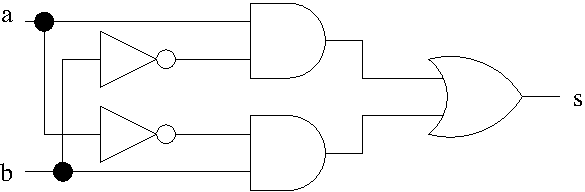
\includegraphics[width=6cm]{ex1.pdf}$$
%\end{enumerate}
%\end{minipage}
%\hfill
%\begin{minipage}[t]{7cm}
%\begin{enumerate}\setcounter{enumi}{1}
\item $a$ et $b$ sont les entrées, $s$ la sortie.
	$$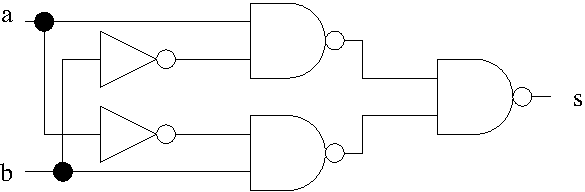
\includegraphics[width=6cm]{ex2.pdf}$$
\end{enumerate}
\end{minipage}
\hfill
\begin{minipage}[t]{7cm}
\begin{enumerate}\setcounter{enumi}{2}
\item $a$ et $b$ sont les entrées, $s$ et $t$ les sorties.	
	$$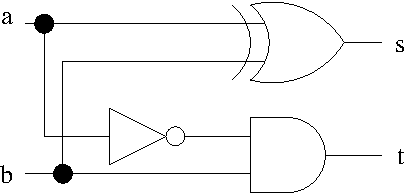
\includegraphics[width=4.5cm]{demiSous.pdf}$$
\item $a$, $b$ et $c$ sont les entrées, $s$ et $t$ les sorties.
	$$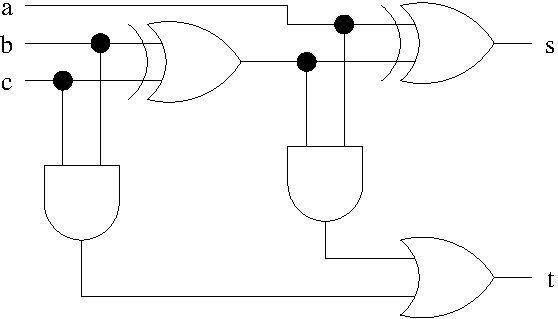
\includegraphics[width=5cm]{add3.pdf}$$
\end{enumerate}
\end{minipage}

\hfill
\begin{minipage}[t]{7cm}
\begin{enumerate}\setcounter{enumi}{4}
\item $a$, $b$ et $c$ sont les entrées et $s$ la sortie.
	$$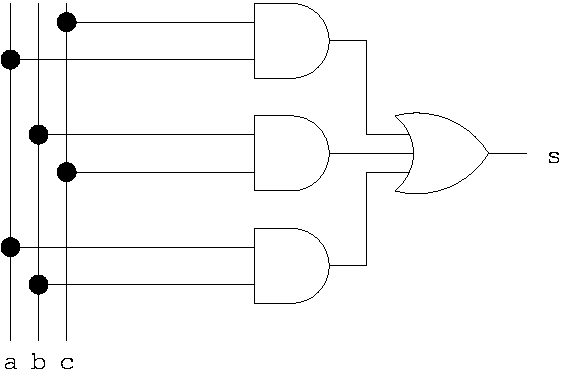
\includegraphics[width=5cm]{majorite.pdf}$$
\item $a$, $b$ et $c$ sont les entrées, $s$ et $t$ les sorties.
	$$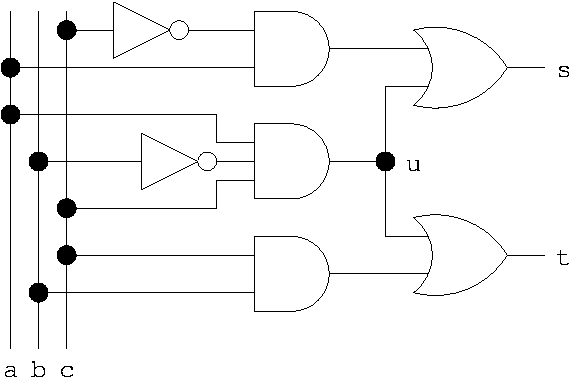
\includegraphics[width=5cm]{circuit.pdf}$$
\end{enumerate}
\end{minipage}
\hfill
\begin{minipage}[t]{7cm}
\begin{enumerate}\setcounter{enumi}{6}
\item $a$, $b$ et $c$ sont les entrées, $s$ la sortie.
	$$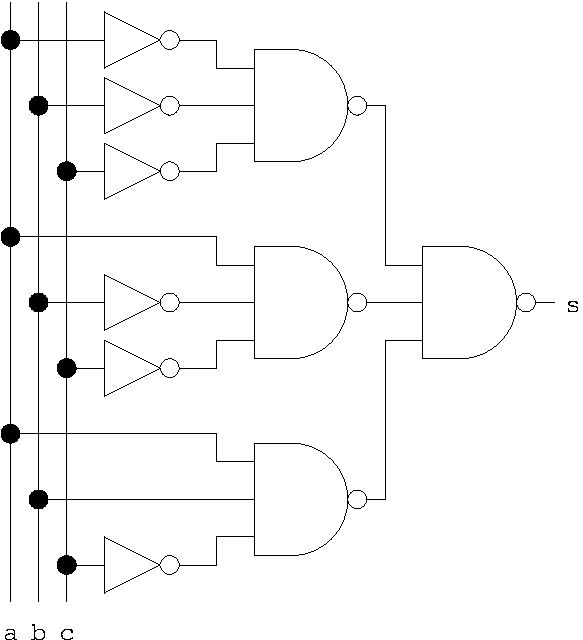
\includegraphics[width=5cm]{f3.pdf}$$
\end{enumerate}
\end{minipage}
\vspace*{3mm}

\begin{minipage}[t]{7cm}
\begin{enumerate}\setcounter{enumi}{7}
\item $a$, $b$ et $c$ sont les entrées, $s_0$,$s_1$\ldots $s_7$ les sorties.
	$$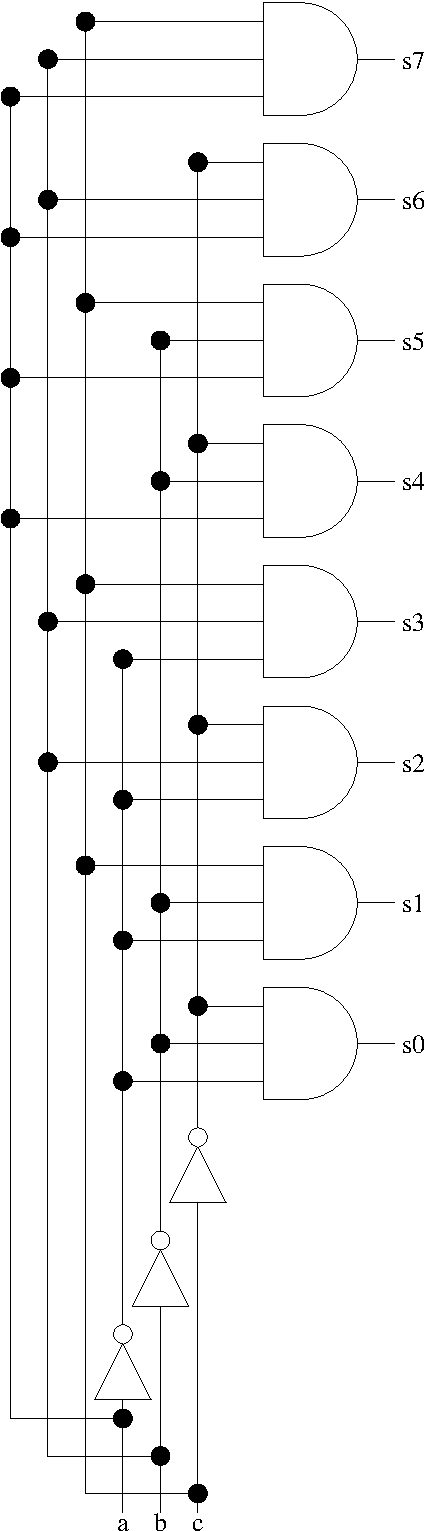
\includegraphics[width=4cm,angle=-90]{decodeur.pdf}$$
\end{enumerate}
\end{minipage}
\end{td}

\begin{td}[Alternative simple et test simple]\label{td:reciproque}\em \index[td]{alternative simple et test simple}
Montrer à l'aide d'un contre-exemple que l'alternative simple :\\
{\tt
\mbox{}\ \ if condition : blocIf\\
\mbox{}\ \ else : blocElse
}\\
n'est pas équivalente à la séquence de tests simples suivante :\\
{\tt
\mbox{}\ \ if condition : blocIf\\
\mbox{}\ \ if not condition : blocElse
}
\end{td}

\begin{td}[Racines du trinome]\label{td:trinome}\em \index[algo]{racines du trinome}\index[td]{racines du trinome}
Ecrire un algorithme qui calcule les racines $x_1$ et $x_2$ du trinome $ax^2 + bx + c$.
\end{td}

\begin{td}[Séquences de tests]\label{td:seq3}\em \index[td]{séquences de tests}
\begin{enumerate}
\item Quelle est la valeur de la variable $x$ après la suite
	d'instructions suivante ?

	{\footnotesize\tt
	x = -3\\
	if x < 0 : x = -x
	}
\item Quelle est la valeur de la variable $y$ après la suite
	d'instructions suivante ?

	{\footnotesize\tt
	x0 = 3\\
	x = 5\\
	if x < x0 : y = -1\\
	else : y = 1
	}
\item Quelle est la valeur de la variable $y$ après la suite
	d'instructions suivante ?

	{\footnotesize\tt
	p = 1\\
	d = 0\\
	r = 0\\
	h = 1\\
	z = 0\\
	f = p and (d or r)\\
	g = not r \\
	m = not p and not z\\
	g = g and (d or h or m)\\
	if f or g : y = 1\\
	else : y = 0
	}
\item Quelle est la valeur de la variable $ok$ après la suite
	d'instructions suivante ?

	{\footnotesize\tt
	x = 2\\
	y = 3\\
	d = 5\\
	h = 4\\
	if x > 0 and x < d :\\
  	\mbox{}\ \ if y > 0 and y < h : ok = 1\\
	\mbox{}\ \ else : ok = 0\\
	else : ok = 0
	}
\item Quelle est la valeur de la variable $y$ après la suite
	d'instructions suivante ?

	{\footnotesize\tt
	x = 3\\
	y = -2\\
	if x < y : y = y - x\\
	elif x == y : y = 0\\
	else : y = x - y
	}
\end{enumerate}
\end{td}
 
\begin{td}[Racine carrée entière]\label{td:racine}\em \index[algo]{racine carrée entière}\index[td]{racine carrée entière}
Ecrire un algorithme qui calcule la racine carrée entière $r$ 
d'un nombre entier positif $n$ telle que $r^2 \leq n < (r+1)^2$.
\end{td}

\begin{td}[Exécutions d'instructions itératives]\label{td:iterations}\em \index[td]{exécutions d'instructions itératives}
\begin{minipage}[t]{7.5cm}
\begin{enumerate}
\item Que fait cette suite d'instructions ?

	{\footnotesize\tt
	x = 0\\
	while x != 33 :\\
	\mbox{}\ \ x = input('entrer un nombre : ')
	}
\end{enumerate}
\end{minipage}
\hfill
\begin{minipage}[t]{7cm}
\begin{enumerate}\setcounter{enumi}{1}
\item Que fait cette suite d'instructions ?

	{\footnotesize\tt
	x = 0\\
	while x <= 0 or x > 5 :\\
	\mbox{}\ \ x = input('entrer un nombre : ')
	}
\end{enumerate}
\end{minipage}

\begin{minipage}[t]{7cm}
\begin{enumerate}\setcounter{enumi}{2}
\item Que fait cette suite d'instructions ?

	{\footnotesize\tt
	s = 0\\
	for i in range(5) :\\
	\mbox{}\ \ x = input('entrer un nombre : ')\\
	\mbox{}\ \ s = s + x
	}
\item Qu'affichent les itérations suivantes ?

	{\footnotesize\tt
	for i in range(0,10) :\\
	\mbox{}\ \ for j in range(0,i) :\\
	\mbox{}\ \ \ \ print('*',end=' ')\\
	\mbox{}\ \ print()
	}
\item Qu'affichent les itérations suivantes ?

	{\footnotesize\tt
	for i in range(0,10) :\\
	\mbox{}\ \ j = 10 - i\\
	\mbox{}\ \ while j > 0 :\\
	\mbox{}\ \ \ \ print('*',end=' ')\\
	\mbox{}\ \ \ \ j = j - 1\\
	\mbox{}\ \ print()
	}
\item Qu'affichent les itérations suivantes ?

	{\footnotesize\tt
	for i in range(1,10):\\
	\mbox{}\ \ for j in range(0,11) :\\
	\mbox{}\ \ \ \ print(i,'x',j,' = ',i*j)\\
	\mbox{}\ \ print()
	}
\item Qu'affichent les itérations suivantes ?\index[algo]{coefficients du binôme}

	{\footnotesize\tt
	for n in range(10) :\\
  	\mbox{}\ \ for p in range(n+1) :\\
    	\mbox{}\ \ \ \ num = 1\\
    	\mbox{}\ \ \ \ den = 1\\
    	\mbox{}\ \ \ \ for i in range(1,p+1) :\\
      	\mbox{}\ \ \ \ \ \ num = num*(n-i+1)\\
      	\mbox{}\ \ \ \ \ \ den = den*i\\
    	\mbox{}\ \ \ \ c = num/den\\
    	\mbox{}\ \ \ \ print(c,end=' ')\\
  	\mbox{}\ \ print()
	}
\end{enumerate}
\end{minipage}
\hfill
\begin{minipage}[t]{7cm}
\begin{enumerate}\setcounter{enumi}{7}
\item Qu'affichent les itérations suivantes ?\index[algo]{nombres de {{\sc Fibonacci}}}

	{\footnotesize\tt
	for n in range(0,15) :\\
  	\mbox{}\ \ f = 1\\
  	\mbox{}\ \ f1 = 1\\
  	\mbox{}\ \ f2 = 1\\
  	\mbox{}\ \ for i in range(2,n+1) :\\
    	\mbox{}\ \ \ \ f = f1 + f2\\
    	\mbox{}\ \ \ \ f2 = f1\\
    	\mbox{}\ \ \ \ f1 = f\\
  	\mbox{}\ \ print(f,end=' ')
	}
\item Quelle est la valeur de la variable $s$
	à la fin des instructions suivantes ?\index[algo]{codage en base $b$}

	{\footnotesize\tt
	b = 2\\
	k = 8\\
	n = 23\\
	s = 0\\
	i = k - 1\\
	q = n\\
	while q != 0 and i >= 0 :\\
  	\mbox{}\ \ s = s + (q\%b)*b**(k-1-i)\\
  	\mbox{}\ \ print(q\%b,end=' ')\\
  	\mbox{}\ \ q = q/b\\
  	\mbox{}\ \ i = i - 1
	}
\end{enumerate}
\end{minipage}
\end{td}


\begin{td}[Figures géométriques]\label{td:geometrieInstruc}\em \index[td]{figure géométrique}
\begin{enumerate}
\item Ecrire un algorithme qui calcule le périmètre $p$ et la surface $s$ d'un rectangle de longueur
	$L$ et de largeur $l$.
\item Ecrire un algorithme qui calcule le périmètre $p$ et la surface $s$ d'un cercle de rayon $r$.
\item Ecrire un algorithme qui calcule la surface latérale $s$ et le volume $v$ d'un cylindre de rayon $r$
	et de hauteur $h$.
\item Ecrire un algorithme qui calcule la surface $s$ et le volume $v$ d'une sphère de rayon $r$.
\end{enumerate}
\end{td}

\begin{td}[Suites numériques]\label{td:suites}\em \index[algo]{suites numériques}\index[td]{suites numériques}
\begin{enumerate}
\item Ecrire un algorithme qui calcule la somme $s = \sum_0^n u_k$ des $n$ premiers termes d'une suite 
	arithmétique $u_k = a + bk$.
\item Ecrire un algorithme qui calcule la somme $s = \sum_0^n u_k$ des $n$ premiers termes d'une suite 
	géométrique $u_k = ab^k$.
\end{enumerate}
\end{td}

\begin{td}[Calcul vectoriel]\label{td:vecteurs}\em \index[algo]{calcul vectoriel}\index[td]{calcul vectoriel}
\begin{enumerate}
\item Ecrire un algorithme qui calcule le module $r$ et les cosinus directeurs $a$, $b$ et $c$
	d'un vecteur de composantes $(x,y,z)$.
\item Ecrire un algorithme qui calcule le produit scalaire $p$ de 2 vecteurs de composantes
	respectives $(x_1,y_1,z_1)$ et $(x_2,y_2,z_2)$.
\item Ecrire un algorithme qui calcule les composantes $(x_3,y_3,z_3)$ du produit vectoriel
	de 2 vecteurs de composantes respectives $(x_1,y_1,z_1)$ et $(x_2,y_2,z_2)$.
\item Ecrire un algorithme qui calcule le produit mixte $v$ de 3 vecteurs de composantes
	respectives $(x_1,y_1,z_1)$, $(x_2,y_2,z_2)$ et $(x_3,y_3,z_3)$.
\end{enumerate}
\end{td}

\begin{td}[Prix d'une photocopie]\label{td:photocopie}\em \index[td]{prix d'une photocopie}
Ecrire un algorithme qui affiche le prix de $n$ photocopies sachant que
	le reprographe facture 0,10 E les dix premières photocopies, 0,09 E 
	les vingt suivantes et 0,08 E au-delà.
\end{td} 

\begin{td}[Calcul des impôts]\label{td:impot}\em \index[td]{calcul des impôts}
Ecrire un algorithme qui affiche si un contribuable d'un pays imaginaire
	est imposable ou non sachant que :
	\begin{itemize}
	\item les hommes de plus de 18 ans paient l'impôt,
    	\item les femmes paient l'impôt si elles ont entre 18 et 35 ans,
	\item les autres ne paient pas d'impôt.
	\end{itemize}
\end{td}


\begin{td}[Développements limités]\label{td:dev}\em \index[algo]{développements limités}\index[td]{développements limités}
Calculer chaque fonction ci-dessous en fonction de son d\'eveloppement 
en série entière ($\sum u_k$). Les calculs seront arr\^et\'es lorsque la 
valeur absolue du terme $u_k$ sera inf\'erieure \`a un certain seuil $s$ 
($0 < s < 1$).\\
On n'utilisera ni la fonction {\em puissance} ($x^n$) ni la fonction 
{\em facto\-riel\-le} ($n!$).
\begin{enumerate}
\item $\displaystyle\sinh(x) \approx \sum_{k=0}^{n} \frac{x^{2k+1}}{(2k+1)!} = 
	x + \frac{x^3}{6} + \frac{x^5}{120} + \ldots + \frac{x^{2n+1}}{(2n+1)!}$
\item $\displaystyle\cosh(x) \approx \sum_{k=0}^{n} \frac{x^{2k}}{(2k)!} = 
	1 + \frac{x^2}{2} + \frac{x^4}{24} + \ldots + \frac{x^{2n}}{(2n)!}$
\item $\displaystyle\cos(x) \approx \sum_{k=0}^{n} (-1)^k\frac{x^{2k}}{(2k)!} = 
	1 - \frac{x^2}{2} + \frac{x^4}{24} + \ldots + (-1)^n\frac{x^{2n}}{(2n)!}$
\item $\displaystyle\log(1+x) \approx \sum_{k=0}^{n} (-1)^k\frac{x^{k+1}}{k+1} = 
	x - \frac{x^2}{2} + \frac{x^3}{3} + \ldots + (-1)^n\frac{x^{n+1}}{n+1}$\ , 
	pour $-1 < x < 1$
\item $\displaystyle\arctan(x) \approx \sum_{k=0}^{n} (-1)^k \frac{x^{2k+1}}{(2k+1)} = 
	x - \frac{x^3}{3} + \frac{x^5}{5} + \ldots + (-1)^n \frac{x^{2n+1}}{(2n+1)}$\ , 
	pour $-1 < x < 1$
\end{enumerate}
\end{td}

\begin{td}[Tables de vérité]\label{td:tablesVerite}\em \index[td]{tables de vérité}
A l'aide d'itérations imbriquées, afficher les tables de vérité des circuits
	logiques du TD \ref{td:circuits2} page \pageref{td:circuits2}.
\end{td}

\begin{td}[Dessins géométriques]\label{td:dessins}\em \index[td]{dessins géométriques}
\begin{minipage}[t]{7cm}
	\begin{enumerate}
	\item Que dessine la suite d'instructions suivante ?

		{\footnotesize\tt
		forward(20)\\
		right(144)\\
		forward(20)\\
		right(144)\\
		forward(20)\\
		right(144)\\
		forward(20)\\
		right(144)\\
		forward(20)\\
		right(144)
		}
	\end{enumerate}
\end{minipage}
\hfill
\begin{minipage}[t]{7cm}
	\begin{enumerate}\setcounter{enumi}{1}
	\item Que dessine la suite d'instructions suivante ?

		{\footnotesize\tt 
		forward(10)\\
		left(45)\\
		forward(10)\\
		left(135)\\
		forward(10)\\
		left(45)\\
		forward(10)\\
		left(135)
		}
	\end{enumerate}
\end{minipage}
\end{td}

\begin{td}[Police d'assurance]\label{td:assurance}\em \index[td]{police d'assurance}
Une compagnie d'assurance automobile propose 4 familles de tarifs du moins
	cher au plus onéreux : A, B, C et D. 
	Le tarif dépend de la situation du conducteur.
	\begin{itemize}
	\item Un conducteur de moins de 25 ans et titulaire du permis depuis 
		moins de deux ans, se voit attribuer le tarif D 
		s'il n'a jamais été responsable d'accident. 
		Sinon, la compagnie refuse de l'assurer.
	\item Un conducteur de moins de 25 ans et titulaire du permis depuis plus de deux ans, 
		ou de plus de 25 ans mais titulaire du permis depuis moins de deux ans 
		a le droit au tarif C s'il n'a jamais provoqué d'accident, 
		au tarif D pour un accident, sinon il est refusé.
	\item Un conducteur de plus de 25 ans titulaire du permis depuis plus de deux ans 
		bénéficie du tarif B s'il n'est à l'origine d'aucun accident 
		et du tarif C pour un accident, du tarif D pour deux accidents, 
		et refusé sinon.
	\end{itemize}
	Par ailleurs, pour encourager la fidélité de ses clients, 
	la compagnie propose un contrat au tarif immédiatement inférieur 
	s'il est assuré depuis plus d'un an.
	
	Ecrire un algorithme qui propose un tarif d'assurance selon les caractéristiques
	d'un client potentiel.
\end{td}


\begin{td}[Zéro d'une fonction]\label{td:zero}\em \index[algo]{zéro d'une fonction}\index[td]{zéro d'une fonction}
On recherche le zéro d'une fonction $f$ continue sur un 
intervalle $[a,b]$ telle que $f(a).f(b) < 0$;
il existe donc une racine de $f$ dans $]a,b[$ que nous supposerons 
unique. 

\begin{enumerate}
\item Ecrire un algorithme qui détermine le zéro de $\cos(x)$ dans $[1,2]$
	selon la méthode par dichotomie.
	
	Indications : on pose $x_1 = a$, $x2 = b$ et $x = (x_1+x_2)/2$. 
	Si $f(x1).f(x) < 0$, la racine est dans $]x_1,x[$ et on pose $x_2 = x$; 
	sinon la racine est dans $]x,x_2[$ et on pose $x_1 = x$. 
	Puis on réitère le procédé, la longueur de l'intervalle ayant été 
	divisée par deux. Lorsque $x_1$ et $x_2$ seront suffisamment proches, 
	on décidera que la racine est $x$.
	
\item Ecrire un algorithme qui détermine le zéro de $\cos(x)$ dans $[1,2]$
	selon la méthode des tangentes.
	
	Indications : soit $x_n$ une approximation de la racine $c$ recherchée : 
	$f(c) = f(x_n) + (c-x_n)f'(x_n)$; comme $f(c) = 0$, on a : 
	$c = x_n - f(x_n)/f'(x_n)$. Posons $x_{n+1} = x_n - f(x_n)/f'(x_n)$ : 
	on peut considérer que $x_{n+1}$ est une meilleure approximation de $c$ que 
	$x_n$. On recommence le procédé avec $x_{n+1}$  et ainsi de suite jusqu'à ce 
	que $|x_{n+1}-x_n|$ soit inférieur à un certain seuil $s$.
	
\item Ecrire un algorithme qui détermine le zéro de $\cos(x)$ dans $[1,2]$
	selon la méthode des sécantes.

	Indications : reprendre la méthode des tangentes en effectuant 
	l'approximation suivante : $f'(x_n) = (f(x_n)-f(x_{n-1}))/(x_n-x_{n-1})$.
\item Ecrire un algorithme qui détermine le zéro de $\cos(x)$ dans $[1,2]$
	selon la méthode des cordes.

	Indications : reprendre la méthode par dichotomie en prenant pour $x$ 
	le point d'intersection de la corde $AB$ et de l'axe des abscisses : 
	$x = (x_2f(x_1) - x_1f(x_2))/(f(x_1)-f(x_2))$, c'est-à-dire le point obtenu 
	par la méthode des sécantes.

\end{enumerate}
\end{td}



%-------------------------------------------------------------------------
\chapter{Procédures et fonctions}\label{ch:fonctions}
%-------------------------------------------------------------------------
	%-------------------------------------------------------------------------
% td-info-S1-fonctions.tex
%-------------------------------------------------------------------------

\begin{td}[Codage des entiers positifs (1)]\label{td:codageEntier}\index[td]{codage des entiers positifs}
\em
Définir un algorithme qui code sur $k$ chiffres en base $b$ un entier positif 
$n$ du système décimal.

Exemples : 
$\begin{array}[t]{l@{\rightarrow}l}
(38)_{10} & (123)_{5} \\
(83)_{10} & (123)_{8} \\
(291)_{10} & (123)_{16}
\end{array}$
\end{td}

\begin{td}[Codage d'un nombre fractionnaire]\label{td:fraction}\index[td]{codage d'un nombre fractionnaire}
\em
Un nombre fractionnaire ({\em nombre avec des chiffres après la virgule} :
{$(r_nr_{n-1}\ldots r_1r_0.r_{-1}r_{-2}\ldots)_b$})
est défini sur un sous-en\-semble borné, incomplet et fini des rationnels.
Un tel nombre a pour valeur :
$${r_nb^n + r_{n-1}b^{n-1} + \ldots + r_1b^1 + r_0b^0 + r_{-1}b^{-1} + r_{-2}b^{-2} + \ldots}$$
En pratique, le {\em nombre de chiffres après la virgule} est limité par la taille physique
en machine.
$${(r_nr_{n-1}\ldots r_1r_0.r_{-1}r_{-2}\ldots r_{-k})_b = \sum_{i=-k}^{i=n} r_ib^i}$$
Un nombre $x$ pourra être représenté en base $b$ par un triplet
$[s,m,p]$ tel que ${x = (-1)^s \cdot m \cdot b^p}$ où $s$ représente le signe de $x$,
$m$ sa mantisse et $p$ son exposant ($p$ comme puissance) où :
\begin{itemize}
\item signe $s$ : $s = 1$ si $x < 0$ et $s = 0$ si $x \geq 0$
\item mantisse $m$ : $m \in [1,b[$ si $x \neq 0$ et $m = 0$ si $x = 0$
\item exposant $p$ : $p \in [min,max]$
\end{itemize}
Ainsi, le codage de $x = -9.75$ en base $b = 2$ s'effectuera en 4
étapes :
\begin{enumerate}
\item coder le signe de $x$ : $x = -9.75 < 0 \Rightarrow {s = 1}$
\item coder la partie entière de $|x|$ : {$9 = (1001)_2$}
\item coder la partie fractionnaire de $|x|$ : {$0.75 = (0.11)_2$}
\item et coder $|x|$ en notation scientifique normalisée : $m \in [1,2[$\\
	$(1001)_2 + (0.11)_2 = (1001.11)_2 = (1.00111)_2\cdot 2^{3}$\\ 
	$= {(1.00111)_2\cdot 2^{{(11)}_2}}$
\end{enumerate}
Cette démarche en 4 étapes conduit au résultat $x = (-1)^s \cdot m \cdot b^p = (-1)^{1} \cdot (1.00111)_2 \cdot 2^{(11)_2}$ où
$b = 2$, $s = (1)_2$, $m = (1.00111)_2$  et $p = (11)_2$.

Déterminer le signe, la mantisse et l'exposant binaires 
du nombre fractionnaire $x = 140.8125$ 
en suivant les 4 étapes décrites ci-dessus.
\end{td}


\begin{td}[Décodage base b $\rightarrow$ décimal]\label{td:decoder}\index[td]{décodage base b $\rightarrow$ décimal}
\em
La valeur décimale d'un nombre entier
codé en base $b$ peut être obtenue par l'algorithme suivant :\\
{\tt \mbox{}\ \ \ \ }\begin{py}{7.5cm}\tt
>>> n = 0\\
>>> for i in range(len(code)):\\
...     n = n + code[i]*b**(len(code)-1-i)\\
... \\
>>> 
\end{py}\\[1mm]
Spécifier une fonction qui encapsulera cet algorithme.
\end{td}

\begin{td}[Codage des entiers positifs (2)]\label{td:codage}\index[td]{codage des entiers positifs}
\em
Définir (spécifier et implémenter) une fonction qui 
code un entier $n$ en base $b$ sur $k$ chiffres
(voir TD \ref{td:codageEntier}).
\end{td}

\begin{td}[Une spécification, des implémentations]\label{td:implem}\index[td]{spécification et implémentations}
\em
\begin{enumerate}
\item Proposer deux implémentations du calcul de
la somme $s = \sum_0^n u_k$ des $n$ premiers termes d'une suite 
géométrique $u_k = a\cdot b^k$.
\item Comparer les complexités de ces deux im\-plé\-men\-ta\-tions.
\end{enumerate}
\end{td}

\begin{td}[Passage par valeur]\label{td:swap}\index[td]{passage par valeur}
\em
On considère les codes suivants :

{\tt \mbox{}\ }\begin{py}{2.25cm}\tt
>>> x, y\\
(1, 2)\\
>>> tmp = x\\
>>> x = y\\
>>> y = tmp\\
>>> x, y\\
(2, 1)
\end{py}
\hfill
\begin{py}{3cm}\tt
def swap(x,y):\\
\mbox{}\ \ \ \ tmp = x\\
\mbox{}\ \ \ \ x = y\\
\mbox{}\ \ \ \ y = tmp\\
\mbox{}\ \ \ \ return
\end{py}
\hfill
\begin{py}{2.25cm}\tt
>>> x, y\\
(1, 2)\\
>>> swap(x,y)\\
>>> x, y\\
(1, 2)
\end{py}\\[1mm]
Expliquer la différence entre l'exécution de gauche et l'exécution de droite
en explicitant l'appel équivalent à l'appel {\tt swap(x,y)} dans l'exécution
de droite.
\end{td}

\begin{td}[Valeurs par défaut]\label{td:defaut}\index[td]{valeurs par défaut}
\em
On considère la fonction qui code en base $b$ sur $k$ chiffres
un nombre décimal $n$ (voir TD \ref{td:codage}). 
Proposer une définition de cette fonction où $k = 8$ et $b = 2$ par défaut.
\end{td}

\begin{td}[Portée des variables]\label{td:portee}\index[td]{portée des variables}
\em
On considère les fonctions {\tt f}, {\tt g} et {\tt h} suivantes :

\begin{py}{2.5cm}\tt
def f(x):\\
\mbox{}\ \ x = 2*x\\
\mbox{}\ \ print('f', x)\\
\mbox{}\ \ return x
\end{py}
\hfill
\begin{py}{2.5cm}\tt
def g(x):\\
\mbox{}\ \ x = 2*f(x)\\
\mbox{}\ \ print('g', x)\\
\mbox{}\ \ return x
\end{py}
\hfill
\begin{py}{2.5cm}\tt
def h(x):\\
\mbox{}\ \ x = 2*g(f(x))\\
\mbox{}\ \ print('h', x)\\
\mbox{}\ \ return x
\end{py}
\mbox{}\vspace*{2mm}

Qu'affichent les appels suivants ?\\
\mbox{}\\
\begin{minipage}{3.5cm}
\begin{enumerate}
\item 
\begin{py}{2.5cm}\tt
>>> x = 5\\
>>> print(x)\\
{\color{red} ?}\\
>>> y = f(x)\\
>>> print(x)\\
{\color{red} ?}\\
>>> z = g(x)\\
>>> print(x)\\
{\color{red} ?}\\
>>> t = h(x)\\
>>> print(x)\\
{\color{red} ?}
\end{py}
\end{enumerate}
\end{minipage}
\hfill
\begin{minipage}{3.5cm}
\begin{enumerate}\setcounter{enumi}{1}
\item 
\begin{py}{2.5cm}\tt
>>> x = 5\\
>>> print(x)\\
{\color{red} ?}\\
>>> x = f(x)\\
>>> print(x)\\
{\color{red} ?}\\
>>> x = g(x)\\
>>> print(x)\\
{\color{red} ?}\\
>>> x = h(x)\\
>>> print(x)\\
{\color{red} ?}
\end{py}
\end{enumerate}
\end{minipage}
\end{td}


\begin{td}[Tours de Hanoï {\em à la main}]\label{td:hanoi}\index[td]{tours de Hanoï}
\em
Résoudre {\em à la main} le problème des tours de Hanoï à $n$ disques
(voir figure \ref{fig:hanoi}) successivement 
pour $n=1$, $n=2$, $n=3$ et $n=4$.
\end{td}
\begin{fig}[Tours de Hanoï (1)]\label{fig:hanoi}
{\bf Etat initial :}\\
\centerline{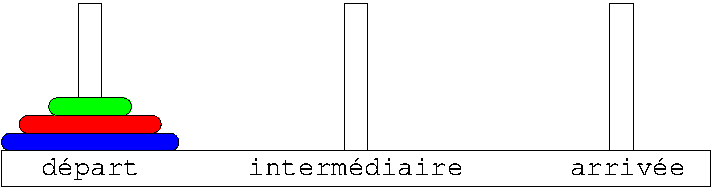
\includegraphics[width=6cm]{hanoi.pdf}}

\noindent{\bf Etat final :}\\
\centerline{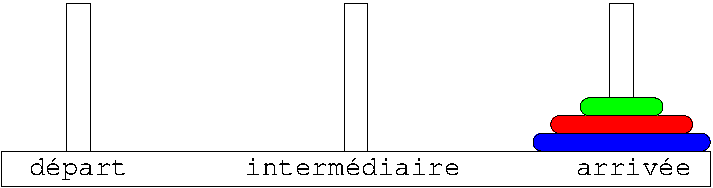
\includegraphics[width=6cm]{hanoi1.pdf}}
\end{fig}



\begin{td}[Pgcd et ppcm de 2 entiers (1)]\label{td:pgcd}\index[td]{pgcd et ppcm de 2 entiers}
\em
\begin{enumerate}
\item Définir une fonction récursive qui calcule le plus grand commun 
	diviseur $d$ de 2 entiers $a$ et $b$ : \\
	$\rm{pgcd}(a,b) = \rm{pgcd}(b,a \bmod b) = \ldots = \rm{pgcd}(d,0) = d$.
\item En déduire une fonction qui calcule le plus petit commun multiple $m$ de 2 entiers $a$ et $b$.
\end{enumerate}
\end{td}

\begin{td}[Somme arithmétique]\label{td:somme}\index[td]{suite arithmétique}
\em
\begin{enumerate}
\item Définir une fonction récursive qui calcule la somme des $n$ premiers
	nombres entiers.
	$$s = \sum^{n}_{k=0}k = \frac{n(n+1)}{2}$$
\item Comparer la complexité de cette version avec les versions constante
	et itérative (voir TD \ref{td:implem}).
\end{enumerate}
\end{td}

\begin{td}[Courbes fractales]\label{td:fractal}\index[algo]{courbes fractales}\index[td]{courbes fractales}
\em
On s'intéresse ici aux programmes dont l'exécution produit des dessins
à l'aide de la tortue Logo.
On consid\`ere la proc\'edure {\tt draw} ci-dessous :

\mbox{}\ \ \begin{py}{7cm}\tt
def draw(n,d):\\
\mbox{}\ \ \ \ assert type(n) is int\\
\mbox{}\ \ \ \ assert n >= 0\\
\mbox{}\ \ \ \ if n == 0: forward(d)\\
\mbox{}\ \ \ \ else:\\
\mbox{}\ \ \ \ \ \ \ \ draw(n-1,d/3.)\\
\mbox{}\ \ \ \ \ \ \ \ left(60)\\
\mbox{}\ \ \ \ \ \ \ \ draw(n-1,d/3.)\\
\mbox{}\ \ \ \ \ \ \ \ right(120)\\
\mbox{}\ \ \ \ \ \ \ \ draw(n-1,d/3.)\\
\mbox{}\ \ \ \ \ \ \ \ left(60)\\
\mbox{}\ \ \ \ \ \ \ \ draw(n-1,d/3.)\\
\mbox{}\ \ \ \ return
\end{py}\\[1mm]
Dessiner le résultat des appels {\tt draw(n,900)} respectivement pour {\tt n = 0},
	{\tt n = 1}, {\tt n = 2} et {\tt n = 3}. A chaque appel, le crayon est 
	initialement en $(0,0)$ avec une direction de $0$.
\end{td}

\begin{td}[QCM (3)]\label{td:qcm3}\index{evaluation@évaluation!contrôle d'attention}
\index{fonction!qcm}\index[td]{contrôle d'attention} (un seul item correct par question)
\em
\begin{enumerate}
\item La réutilisabilité d'un algorithme est son aptitude
	\begin{enumerate}
	\item à utiliser de manière optimale les ressources du matériel qui l'exécute
	\item à se protéger de conditions anormales d'utilisation
	\item à résoudre des tâches équivalentes à celle pour laquelle il a été conçu
	\item à réaliser exactement la tâche pour laquelle il a été conçu
	\end{enumerate}

\item L'encapsulation est l'action
	\begin{enumerate}
	\item de mettre une chose dans une autre
	\item de fermer une chose par une autre
	\item de substituer une chose par une autre
	\item de remplacer une chose par une autre
	\end{enumerate}
	
\item Une fonction est un bloc d'instructions nommé et paramétré 
	\begin{enumerate}
	\item qui ne peut pas retourner plusieurs valeurs
	\item qui ne peut pas contenir d'instructions itératives
	\item qui retourne une valeur
	\item qui ne retourne pas de valeur
	\end{enumerate}

\item Les paramètres d'entrée d'une fonction sont
	\begin{enumerate}
	\item les arguments nécessaires pour effectuer le traitement associé à la fonction
	\item les valeurs obtenues après avoir effectué le traitement associé à la fonction
	\item des grandeurs invariantes pendant l'exécution de la fonction
	\item des variables auxiliaires définies dans le corps de la fonction
	\end{enumerate}
	
\item Les préconditions d'une fonction sont des conditions à respecter 
	\begin{enumerate}
	\item par les paramètres de sortie de la fonction
	\item pendant toute l'exécution de la fonction
	\item par les paramètres d'entrée de la fonction
	\item pour pouvoir compiler la fonction
	\end{enumerate}
	
\item La description d'une fonction décrit
	\begin{enumerate}
	\item ce que fait la fonction
	\item comment fait la fonction
	\item pourquoi la fonction le fait 
	\item où la fonction le fait
	\end{enumerate}
	
\item Le jeu de tests d'une fonction est 
	\begin{enumerate}
	\item un ensemble d'exercices à résoudre
	\item un ensemble d'exceptions dans le fonctionnement de la fonction
	\item un ensemble caractéristiques d'entrées-sorties associées
	\item un ensemble de recommandations dans l'utilisation de la fonction
	\end{enumerate}

\item En {\sc Python}, l'instruction {\tt assert} permet de 
	\begin{enumerate}
	\item tester une précondition
	\item imposer une instruction
	\item paramétrer une fonction
	\item tester un test du jeu de tests
	\end{enumerate}

\item La validité d'une fonction est son aptitude à réaliser exactement 
	la tâche pour laquelle elle a été conçue. Plus concrètement,
	\begin{enumerate}
	\item la fonction doit vérifier impérativement ses préconditions
	\item la fonction doit être correctement paramétrée
	\item l'implémentation de la fonction doit être conforme aux jeux de tests
	\item l'utilisation de la fonction doit être conviviale
	\end{enumerate}

\item Le passage des paramètres par valeur consiste à copier
	\begin{enumerate}
	\item la valeur du paramètre formel dans le paramètre effectif correspondant
	\item la référence du paramètre effectif dans le paramètre formel correspondant
	\item la référence du paramètre formel dans le paramètre effectif correspondant
	\item la valeur du paramètre effectif dans le paramètre formel correspondant
	\end{enumerate}
	
\item Un appel récursif est un appel 
	\begin{enumerate}
	\item dont l'exécution est un processus récursif
	\item dont l'exécution est un processus itératif
	\item dont le résultat est retourné par la fonction
	\item d'une fonction par elle-même
	\end{enumerate}	
\end{enumerate}
\end{td}


\begin{td}[Passage des paramètres]\label{td:passage}\index{fonction!passage par valeur}\index[td]{passage par valeur}
\em
On considère les fonctions {\tt f}, {\tt g} et {\tt h} suivantes :

\begin{center}
\begin{py}{4cm}
\begin{verbatim}
def f(x):
    y = x + 2
    return y
\end{verbatim}
\end{py}\hspace*{1cm}
\begin{py}{4cm}
\begin{verbatim}
def g(z):
    v = 2*f(z)
    return v
\end{verbatim}
\end{py}\hspace*{1cm}
\begin{py}{4cm}
\begin{verbatim}
def h(a):
    b = g(f(a))
    return b
\end{verbatim}
\end{py}
\end{center}

Quels sont les algorithmes équivalents (algorithmes où il n'y a plus 
d'appels aux fonctions {\tt f}, {\tt g} et {\tt h}) aux appels suivants :
\vspace*{2mm}

\begin{minipage}{4cm}
\begin{enumerate}
\item {\tt u = f(2)}
\item {\tt u = f(t)}
\end{enumerate}
\end{minipage}\hfill
\begin{minipage}{4cm}
\begin{enumerate}\setcounter{enumi}{2}
\item {\tt u = g(2)}
\item {\tt u = g(t)}
\end{enumerate}
\end{minipage}\hfill
\begin{minipage}{4cm}
\begin{enumerate}\setcounter{enumi}{4}
\item {\tt u = h(2)}
\item {\tt u = h(t)}
\end{enumerate}
\end{minipage}

\end{td}

\begin{td}[Portée des variables (2)]\label{td:portee2}\index{variable!portée}\index[td]{portée des variables}
\em
On considère les fonctions {\tt f}, {\tt g} et {\tt h} suivantes :
\begin{center}
\begin{py}{4cm}
\begin{verbatim}
def f(x):
    x = x + 2
    print('f', x)
    return x
\end{verbatim}
\end{py}\hspace*{1cm}
\begin{py}{4cm}
\begin{verbatim}
def g(x):
    x = 2*f(x)
    print('g', x)
    return x
\end{verbatim}
\end{py}\hspace*{1cm}
\begin{py}{4cm}
\begin{verbatim}
def h(x):
    x = g(f(x))
    print('h', x)
    return x
\end{verbatim}
\end{py}
\end{center}

Qu'affichent les appels suivants ?
\vspace*{2mm}

\begin{minipage}[t]{7cm}
\begin{enumerate}
\item 

\begin{py}{4cm}
\begin{verbatim}
>>> x = 5
>>> print(x)

>>> x = x + 2
>>> print(x)

>>> x = 2 * (x + 2)
>>> print(x)

\end{verbatim}
\end{py}

\item 

\begin{py}{4cm}
\begin{verbatim}
>>> x = 5
>>> print(x)

>>> y = f(x)
>>> print(x, y)

>>> z = 2*f(y)
>>> print(x, y, z)

\end{verbatim}
\end{py}


\item 

\begin{py}{4cm}
\begin{verbatim}
>>> x = 5
>>> print(x)

>>> z = 2*f(f(x))
>>> print(x, z)

\end{verbatim}
\end{py}


\end{enumerate}
\end{minipage}\hfill
\begin{minipage}[t]{7cm}
\begin{enumerate}\setcounter{enumi}{3}
\item 

\begin{py}{4cm}
\begin{verbatim}
>>> x = 5
>>> print(x)

>>> f(x)

>>> print(x)

>>> g(x)

>>> print(x)

>>> h(x)

>>> print(x)

\end{verbatim}
\end{py}


\end{enumerate}
\end{minipage}
\end{td}


\begin{td}[Suite géométrique]\label{td:geometrie}\index[algo]{suites numériques}\index[td]{suite
géométriques}
\em
Définir une fonction récursive qui calcule la somme des $n$ premiers termes 
d'une suite géométrique $u_k = ab^k$.
\end{td}

\begin{td}[Puissance entière]\label{td:puissance}\index[algo]{fonction puissance}\index[td]{fonction puissance}
\em
Définir une fonction récursive qui calcule la puissance entière $p = x^n$ 
d'un nombre entier $x$.
\end{td}

\begin{td}[Coefficients du binôme]\label{td:binome}\index[algo]{coefficients du binôme}\index[td]{coefficients du binôme}
\em
Définir une fonction récursive qui calcule les coefficients du binôme :\\
$\displaystyle (a+b)^n = \sum_{k=0}^n \frac{n!}{k!(n-k)!}a^{n-k}b^k$.
\end{td}

\begin{td}[Fonction d'Ackerman]\label{td:ackerman}\index[algo]{fonction d'Ackerman}\index[td]{fonction d'Ackerman}\index{{{\sc Ackerman}}}
\em
Définir une fonction récursive qui calcule la fonction d'Ackerman : 
$$
{f : N^2 \rightarrow N}\ 
\left\{\begin{array}{lll}
f{(0,n)} & = & n+1\\
f{(m,0)} & = & f{(m-1,1)}\mbox{\ si\ } m > 0\\
f{(m,n)} & = & f{(m-1,f{(m,n-1)})}\mbox{\ si\ } m > 0, n > 0
\end{array}\right.
$$
\end{td}

\begin{td}[Addition binaire]\label{td:addition2}\index[algo]{opérations binaires}\index[td]{addition binaire}
\em
Définir une fonction {\tt add2} qui effectue l'addition binaire de 2 
entiers $a$ et $b$ (le nombre de bits n'est pas limité {\em a priori}).\\
Exemple : $(0101)_2 + (10011)_2 = (11000)_2$

\begin{py}{7cm}
\begin{verbatim}
# add2(a,b)
>>> add2([1,0],[1,0,1,1])
[1, 1, 0, 1]
>>> add2([1,0,1,1],[1,0])
[1, 1, 0, 1]
>>> add2([1,1],[1,1])
[1, 1, 0]
\end{verbatim}
\end{py}
\end{td}

\begin{td}[Complément à 2]\label{td:complement2}\index[td]{complément à 2}
\em
Définir une fonction {\tt neg2} qui détermine le complément à 2 en binaire 
d'un entier $n$ codé sur $k$ bits.
	$$(011100)_2 \rightarrow (100100)_2\ :\ \begin{array}[t]{lrr} 
	  & (011100)_2\\
	\hline
	  & (100011)_2\\
	+ & (000001)_2\\
	\hline
	= & (100100)_2
	\end{array}$$

	\begin{py}{7cm}
	\begin{verbatim}
	# neg2(code)
	>>> neg2([0,0,0,1,0,1,1,1])
	[1, 1, 1, 0, 1, 0, 0, 1]
	>>> neg2([1, 1, 1, 0, 1, 0, 0, 1])
	[0, 0, 0, 1, 0, 1, 1, 1]
	>>> for a in [0,1]:
	...    for b in [0,1]:
	...        for c in [0,1]:
	...            add2([a,b,c],neg2([a,b,c]))
	[0, 0, 0]
	[1, 0, 0, 0]
	[1, 0, 0, 0]
	[1, 0, 0, 0]
	[1, 0, 0, 0]
	[1, 0, 0, 0]
	[1, 0, 0, 0]
	[1, 0, 0, 0]
	\end{verbatim}
	\end{py}
\end{td}

\begin{td}[Codage-décodage des réels]\label{td:ieee754}\index[algo]{codage des réels}\index[td]{codage des réels}\index{norme IEEE 754}
\em

\begin{enumerate}
\item Définir une fonction {\tt ieee} qui code
	un nombre réel $x$ selon la norme IEEE 754 simple précision.
	$$x = (-1)^s\cdot (1+m)\cdot 2^{(e-127)}$$

	\begin{py}{7cm}
	\begin{verbatim}
	# ieee(x)
	>>> ieee(0.0)
	[0, 0, 0, 0, 0, 0, 0, 0, 0, 
	 0, 0, 0, 0, 0, 0, 0, 0, 0, 0, 0, 
	 0, 0, 0, 0, 0, 0, 0, 0, 0, 0, 0, 0]
	>>> ieee(0.625)
	[0, 0, 1, 1, 1, 1, 1, 1, 0, 
	 0, 1, 0, 0, 0, 0, 0, 0, 0, 0, 0, 
	 0, 0, 0, 0, 0, 0, 0, 0, 0, 0, 0, 0]
	>>> ieee(3.1399998664855957)
	[0, 1, 0, 0, 0, 0, 0, 0, 0, 
	 1, 0, 0, 1, 0, 0, 0, 1, 1, 1, 1, 
	 0, 1, 0, 1, 1, 1, 0, 0, 0, 0, 1, 0]
	>>> ieee(-4573.5)
	[1, 1, 0, 0, 0, 1, 0, 1, 1, 
	 0, 0, 0, 1, 1, 1, 0, 1, 1, 1, 0, 
	 1, 1, 0, 0, 0, 0, 0, 0, 0, 0, 0, 0]
	\end{verbatim}
	\end{py}

\item Définir une fonction {\tt real} qui décode un nombre réel $x$ 
	codé selon la norme IEEE 754 simple précision.
	$$x = (-1)^s\cdot (1+m)\cdot 2^{(e-127)}$$

	\begin{py}{7cm}
	\begin{verbatim}
	# real(code)
	>>> real(ieee(0.625))
	0.625
	>>> real(ieee(3.1399998664855957))
	3.1399998664855957
	>>> real(ieee(-4573.5))
	-4573.5
	\end{verbatim}
	\end{py}
\end{enumerate}

\noindent On pourra vérifier les résultats obtenus avec la fonction {\tt ieee}
du TD \ref{td:ieee754} ci-contre sur le site 
\href{http://babbage.cs.qc.edu/IEEE-754/Decimal.html}{\tt http\char`://babbage.cs.qc.edu/IEEE-754/Decimal.html}

\end{td}

\begin{td}[Intégration numérique]\label{td:integration}\index[algo]{intégration numérique}\index[td]{intégration numérique}
\em
Soit $f(x)$ une fonction continue de $R \rightarrow R$ à intégrer sur $[a,b]$ 
(on supposera que $f$ à toutes les bonnes propriétés mathématiques pour être
intégrable sur l'intervalle considéré). On cherche à calculer son intégrale
$\displaystyle I = \int_a^b f(x)dx$ qui représente classiquement l'aire
comprise entre la courbe représentative de $f$ et les droites d'équations 
$x=a$, $x=b$ et $y=0$. Les méthodes d'intégration numérique (méthode des rectangles, 
méthode des trapèzes et méthode de Simpson) consistent 
essentiellement à trouver une bonne approximation de cette aire.
$$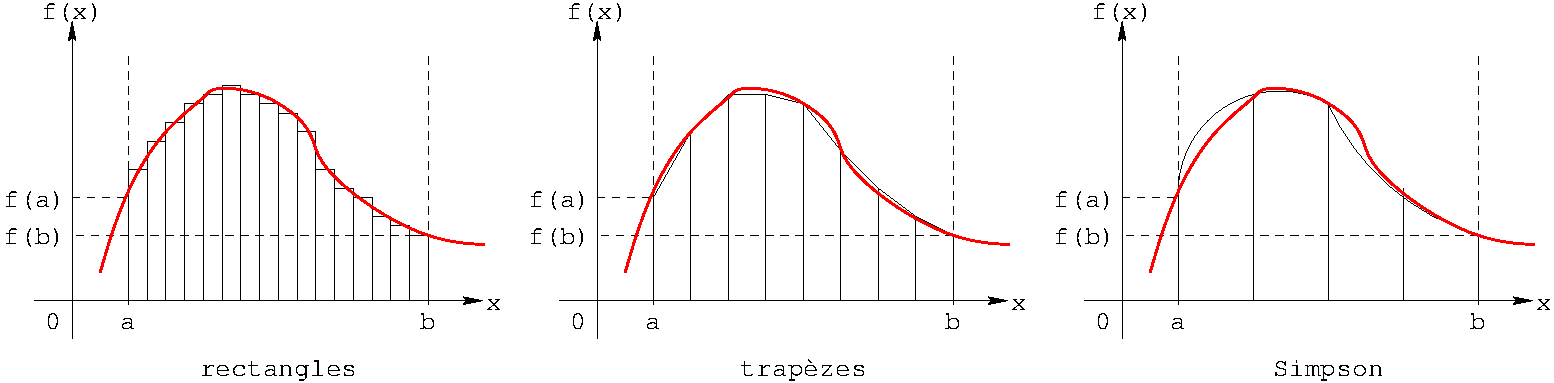
\includegraphics[width=14cm]{integrale.pdf}$$

On testera ces différentes méthodes avec la fonction $f(x) = \sin(x)$ sur $[0,\pi]$.
\begin{enumerate}
\item Méthode des rectangles : subdivisons l'intervalle d'intégration de
	longueur $b-a$ en $n$ parties égales de longueur 
	$\displaystyle\Delta x = \frac{b-a}{n}$. Soient $x_1$, $x_2$, \ldots,
	$x_n$ les points milieux de ces $n$ intervalles. Les $n$ rectangles
	formés avec les ordonnées correspondantes ont pour surface $f(x_1)\Delta
	x$, $f(x_2)\Delta x$, \ldots, $f(x_n)\Delta x$. L'aire sous la courbe 
	est alors assimilée à la somme des aires de ces rectangles, soit 
	$$\displaystyle I = \int_a^b f(x)dx \approx
	\left(f(x_1)+f(x_2)+\cdots+f(x_n)\right)\Delta x$$ 
	C'est la formule dite
	des rectangles qui repose sur une approximation par une fonction {\em en
	escalier}.
	
	Ecrire une fonction {\tt rectangle\_integration} qui calcule l'intégrale définie $I$ d'une fonction 
	$f$ sur $[a,b]$ à l'ordre $n$ par la méthode des rectangles.
	
\item Méthode des trapèzes : subdivisons l'intervalle d'intégration de
	longueur $b-a$ en $n$ parties égales de longueur 
	$\displaystyle\Delta x = \frac{b-a}{n}$. Les abscisses des points ainsi
	définis sont
	$a$, $x_1$, $x_2$, \ldots, $x_{n-1}$, $b$ et les trapèzes construits sur ces
	points et les ordonnées correspondantes ont pour aire 
	$\displaystyle \frac{\Delta x}{2}\left(f(a) + f(x_1)\right)$,
	$\displaystyle \frac{\Delta x}{2}\left(f(x_1) + f(x_2)\right)$,
	\ldots,
	$\displaystyle \frac{\Delta x}{2}\left(f(x_{n-1}) + f(b)\right)$.
	L'aire sous la courbe est alors assimilée à la somme des aires de ces 
	trapèzes, soit
	$$\displaystyle I = \int_a^b f(x)dx \approx
	\left(\frac{f(a)+f(b)}{2} + f(x_1) + f(x_2) + \cdots + f(x_{n-1})\right)
	\Delta x$$
	C'est la formule dite des trapèzes.
	
	Ecrire une fonction {\tt trapezoid\_integration} qui calcule l'intégrale définie $I$ d'une fonction 
	$f$ sur $[a,b]$ à l'ordre $n$ par la méthode des trapèzes.
	
\item Méthode de Simpson : divisons l'intervalle d'intégration $[a,b]$ en un nombre 
	$n$ pair d'inter\-val\-les dont la longueur est 
	$\displaystyle\Delta x = \frac{b-a}{n}$. 
	Dans les 2 premiers intervalles d'extrémités $a$, $x_1$ et $x_2$, on approche 
	la courbe représentative de $f$ par une parabole d'équation 
	$y = \alpha x^2 + \beta x + \gamma$ passant par les points $A(a,f(a))$, 
	$A_1(x_1,f(x_1))$ et $A_2(x_2,f(x_2))$ de la courbe. Dans les 2 intervalles 
	suivants, on approche la courbe par une autre parabole d'équation similaire, 
	passant par les points $A_2$, $A_3$ et $A_4$, et ainsi de suite.
	On obtient ainsi une courbe formée de $n$ portions de parabole et
	l'aire déterminée par ces portions de parabole est une approximation de l'aire $I$
	cherchée.
	
	L'intégration de l'équation de la parabole $y = \alpha x^2 + \beta x + \gamma$ sur
	$\displaystyle \left[-\Delta x,\Delta x\right]$ donne 
	$$S = \int_{-\Delta x}^{\Delta x} (\alpha x^2 + \beta x + \gamma)dx = 
	\frac{2}{3}\alpha(\Delta x)^3 + 2\gamma(\Delta x)$$
	où les constantes $\alpha$ et $\gamma$ sont déterminées en écrivant que les points
	$(-\Delta x,y_0)$, $(0,y_1)$ et $(\Delta x,y_2)$ satisfont l'équation de la parabole.
	On obtient ainsi :
	$$\left|\begin{array}{l@{\ =\ }l}
	y_0 & \alpha(-\Delta x)^2 + \beta(-\Delta x) + \gamma\\
	y_1 & \gamma\\
	y_2 & \alpha(\Delta x)^2 + \beta(\Delta x) + \gamma
	\end{array}\right.
	\Rightarrow
	\left|\begin{array}{l@{\ =\ }l}
	\alpha & \displaystyle \frac{y_0 - 2y_1 + y_2}{2(\Delta x)^2} \\
	\beta  & \displaystyle \frac{y_2-y_0}{2(\Delta x)}\\
	\gamma & \displaystyle y_1
	\end{array}\right.$$
	et $\displaystyle S = \frac{\Delta x}{3}(y_0+4y_1+y_2)$.
	
	Par suite, il vient :
	$\displaystyle\left|\begin{array}{l@{\ =\ }l}
	S_1     & \displaystyle \frac{\Delta x}{3}(y_0 + 4y_1 + y_2)\\
	S_2     & \displaystyle \frac{\Delta x}{3}(y_2 + 4y_3 + y_4)\\
	S_3     & \displaystyle \frac{\Delta x}{3}(y_4 + 4y_5 + y_6)\\
	\vdots  \\
	\displaystyle S_{n/2} & \displaystyle \frac{\Delta x}{3}(y_{n-2} + 4y_{n-1} + y_n)
	\end{array}\right.$ 
	
	d'où
	$$I = \int_a^b f(x)dx \approx \frac{\Delta x}{3}
	\left(f(a) + 4\sum_{i=1,3,5...}^{n-1}f(x_i) + 2\sum_{i=2,4,6...}^{n-2}f(x_i) + f(b)\right)$$
	
	C'est la formule dite de Simpson qui repose sur une approximation de $f$ 
	par des arcs de parabole.\index{{{\sc Simpson}}}

	Ecrire une fonction {\tt simpson\_integration} qui calcule l'intégrale définie $I$ d'une fonction 
	$f$ sur $[a,b]$ à l'ordre $n$ par la méthode de Simpson.
\end{enumerate}
\end{td}

\begin{td}[Tracés de courbes paramétrées]\label{td:traces}\index[algo]{courbes paramétrées}\index[td]{courbes paramétrées}
\em
Une courbe paramétrée dans le plan est une courbe où l'abscisse $x$ et l'ordonnée $y$
sont des fonctions d'un paramètre qui peut être le temps $t$ ou un angle $\theta$ par exemple.
La courbe se présente donc sous la forme $x = f(t), y= g(t)$. Les tableaux ci-dessous en donnent quelques
exemples.

$$\begin{tabular}{|ll|}
\hline
droite & $x = x_0 + \alpha t$\\
       & $y = y_0 + \beta t$\\
\hline
cercle & $x = x_0 + r\cos(\theta)$\\
       & $y = y_0 + r\sin(\theta)$\\
\hline
ellipse & $x = x_0 + a\cos(\phi)$\\
        & $y = y_0 + b\cos(\phi)$ \\
\hline
hyperbole & $\displaystyle x = x_0 + \frac{a}{\cos(\theta)}$ \\
          & $ y = y_0 + b \tan(\theta)$\\
\hline
\end{tabular}
\hspace*{2mm}
\begin{tabular}{|ll|}
\hline
cycloïde & $x = x_0 + r(\phi - \sin(\phi))$\\
       & $y = y_0 + r(1 - \cos(\phi))$\\
\hline
épicycloïde & $\displaystyle x = x_0 + (R+r)\cos(\theta) - r\cos\left(\frac{R+r}{r}\cdot\theta\right)$\\
       & $\displaystyle y = y_0 + (R+r)\sin(\theta) - r\sin\left(\frac{R+r}{r}\cdot\theta\right)$\\
\hline
hypercycloïde & $\displaystyle x = x_0 + (R-r)\cos(\theta) + r\cos\left(\frac{R-r}{r}\cdot\theta\right)$\\
        & $\displaystyle x = y_0 + (R-r)\sin(\theta) + r\sin\left(\frac{R-r}{r}\cdot\theta\right)$ \\
\hline
\end{tabular}$$
$$\begin{tabular}{|ll|}
\hline
limaçon de Pascal & $x = x_0 + (a\cos(\theta) + b)\cos(\theta)$\\
                  & $y = y_0 + (a\cos(\theta) + b)\sin(\theta)$\\
\hline
spirale logarithmique & $\displaystyle x = x_0 + ke^\theta\cos(\theta)$\\
                      & $\displaystyle y = y_0 + ke^\theta\sin(\theta)$\\
\hline
\end{tabular}$$

\begin{fig}[Courbes paramétrées]\label{fig:traces}
$$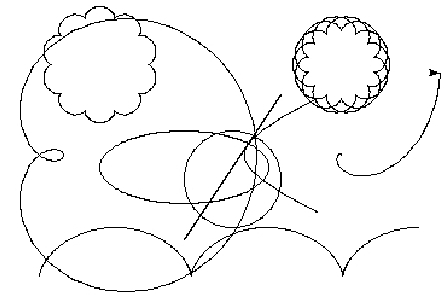
\includegraphics[width=7.5cm]{param2.jpg}$$
\end{fig}
Ecrire une fonction {\tt drawCurve} qui permettent le tracé de telles courbes paramétrées
(figure \ref{fig:traces}).
On utilisera les instructions {\em à la {\sc Logo}} pour réaliser ces tracés
(voir annexe \ref{logo} page \pageref{logo}).
\end{td}


%-------------------------------------------------------------------------
\chapter{Structures linéaires}\label{ch:listes}
%-------------------------------------------------------------------------
	%-------------------------------------------------------------------------
% td-info-S1-listes.tex
%-------------------------------------------------------------------------


\begin{td}[Distance de 2 points de l'espace]\label{td:distance}
\em
Définir la fonction {\tt distance} qui calcule la distance entre 2 points
$M_1$ et $M_2$ de l'espace, respectivement de coordonnées $(x_1,y_1,z_1)$ 
et $(x_2,y_2,z_2)$.
\end{td}

\begin{td}[Opérations sur les n-uplets]\label{td:n-uplet}\index[td]{opérations sur les n-uplets}
\em
Donner un exemple d'utilisation de chacune des opé\-ra\-tions  
sur les n-uplets décrites dans le tableau de la page \pageref{tab:sequences}.
\end{td}

\begin{td}[Pgcd et ppcm de 2 entiers (2)]\label{td:pgcdppcm}\index[td]{pgcd et ppcm de 2 entiers}
(voir TD \ref{td:pgcd})\\
\em
Définir une fonction qui calcule le pgcd et le ppcm de 2 entiers $a$ et $b$.
\end{td}

\begin{td}[Opérations sur les chaînes]\label{td:chaine}\index[td]{opérations sur les chaînes de caractères}
\em
Donner un exemple d'utilisation de chacune des opé\-ra\-tions  
sur les chaînes de caractères décrites dans le tableau de la page \pageref{tab:chaines}.
\end{td}

\begin{td}[Inverser une chaîne]\label{td:inverser}\index[td]{inverser une chaîne}
\em
Définir une fonction qui crée une copie d'une chaîne en inversant l'ordre des caractères.

\noindent\mbox{}\hspace*{1cm}\begin{py}{6cm}\tt
>>> inverser('inverser')\\
'resrevni'
\end{py}
\end{td}

\begin{td}[Caractères, mots, lignes d'une chaîne]\label{td:wc}\index[td]{caractères, mots, lignes d'une chaîne}
\em
Définir une fonction qui compte le nombre de caractères, le nombre de mots et le nombres de lignes
d'une chaîne de caractères.
\end{td}

\begin{td}[Opérations sur les listes (1)]\label{td:listes1}\index[td]{opérations sur les listes}
\em
Donner un exemple d'utilisation de chacune des opé\-ra\-tions  
sur les listes décrites dans le tableau de la page \pageref{tab:listes}.
\end{td}

\begin{td}[Opérations sur les listes (2)]\label{td:listes2}
\em
Vérifier que les opérations suivantes sont équivalentes deux à deux :
$$\begin{tabular}{l@{ et }l}
{\tt del s[i\char`:j]}	& {\tt s[i\char`:j] = []}\\
{\tt s.append(x)}	& {\tt s[len(s)\char`:len(s)] = [x]}\\
{\tt s.extend(x)}      	& {\tt s[len(s)\char`:len(s)]= x}\\
{\tt s.insert(i,x)}	& {\tt s[i\char`:i] = [x]}\\
{\tt s.remove(x)}	& {\tt del s[s.index(x)]}\\
{\tt s.pop(i)}		& {\tt x = s[i]; del s[i]}\\
\end{tabular}$$
\end{td}


\begin{td}[Sélection d'éléments]\label{td:collect}\index[td]{sélection d'éléments}
\em
\begin{enumerate}
\item Définir une fonction qui crée une liste {\tt t} composée des éléments d'une autre 
	liste {\tt s} qui vérifient une certaine condition {\tt p} ({\tt p(s[i]) == True}).
\item Définir une fonction qui supprime d'une liste {\tt s} les éléments qui ne vérifient
	pas une certaine condition {\tt p}.
\end{enumerate}
\end{td}

\begin{td}[Opérations sur les piles]\label{td:pile}\index[td]{opérations sur les piles}
\em
Définir les 4 opérations sur les piles définies ci-contre~: {\tt emptyStack}, {\tt topStack},
{\tt pushStack} et {\tt popStack}. On empilera et dépilera à la fin de la liste qui
sert à stocker les éléments de la pile.
\end{td}

\begin{td}[Opérations sur les files]\label{td:file}\index[td]{opérations sur les files}
\em
Définir les 4 opérations sur les files définies ci-contre~: {\tt emptyQueue}, {\tt topQueue},
{\tt pushQueue} et {\tt popQueue}. On enfilera en début de liste et on défilera à la fin de la liste qui
sert à stocker les éléments de la file.
\end{td}

\begin{td}[Produit de matrices]\label{td:matrices1}\index[td]{opérations sur les matrices}
\em
Définir la fonction qui calcule la matrice $C$, produit 
de 2 matrices $A$ et $B$ respectivement de dimensions $(n,r)$ et $(r,m)$.
$$c_{i,j} = \sum_{k=0}^{r-1}a_{ik}\cdot b_{kj}$$
\centerline{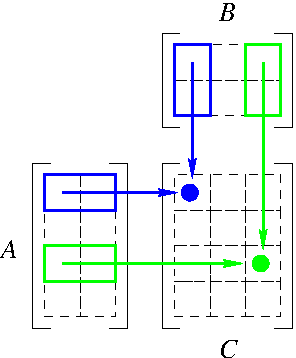
\includegraphics[width=4cm]{produit-matrices.pdf}}
\end{td}

\begin{td}[Annuaire téléphonique]\label{td:annuaire}\index[td]{annuaire téléphonique}
\em
On considère un annuaire téléphonique stocké sous la forme d'une liste de couples
{\tt (nom, téléphone)} (exemple : {\tt [('jean','0607080910'),('paul','0298000102')]}).
\begin{enumerate}
\item Définir une fonction qui retrouve dans un annuaire téléphonique
	le numéro de téléphone à partir du nom.
\item Définir la fonction inverse qui retrouve 
	le nom à partir du numéro de téléphone.
\end{enumerate}
\end{td}

\begin{td}[Recherche dichotomique]\label{td:dicho}\index[td]{recherche dichotomique}
\em
La recherche dichotomique présentée ci-contre n'assure pas de trouver la première occurence
d'un élément {\tt x} dans une liste {\tt t} triée.\\
Modifier l'algorithme de recherche dichotomique proposé pour rechercher la
première occurence d'un élément {\tt x} dans une liste {\tt t} triée.
\end{td}

\begin{td}[Liste ordonnée]\label{td:enordre}\index[td]{liste ordonnée}
\em
Définir une version itérative de la fonction récursive {\tt enOrdre}
définie ci-dessous. On appliquera la méthode de transformation décrite en
section \ref{methode:recursivite} page \pageref{methode:recursivite}.

\footnotesize
\begin{verbatim}
def enOrdre(t,debut,fin):
    assert type(t) is list
    assert 0 <= debut <= fin < len(t)
    ok = False
    if debut == fin: ok = True
    else:
        if t[debut] <= t[debut+1]: 
            ok = enOrdre(t,debut+1,fin)
    return ok
\end{verbatim}

\end{td}

\begin{td}[Tri d'un annuaire téléphonique]\label{td:tri1}\index[td]{tri d'un annuaire}
\em
On considère un annuaire téléphonique stocké sous la forme d'une liste de couples
{\tt (nom, téléphone)} (exemple : {\tt [('paul','0607080910'),('jean','0298000102')]}).

Définir une fonction qui trie un annuaire téléphonique par ordre alphabétique des noms.
\end{td}

\begin{td}[Complexité du tri par sélection]\label{td:tri2}\index[td]{complexité du tri par sélection}
\em
Montrer que la complexité du tri par sélection est :
\begin{enumerate}
\item en $O(n)$ en ce qui concerne les échanges de valeurs au sein d'une liste
	de longueur $n$,
\item en $O(n^2)$ en ce qui concerne les comparaisons entre éléments de la liste.
\end{enumerate}
\end{td}

\begin{td}[Tri par insertion]\label{td:tri3}\index[td]{tri par insertion}
\em
Exécuter à la main l'appel {\tt triInsertion([9,8,7,6,5,4],1,4)} en donnant
les valeurs des variables {\tt i}, {\tt k}, {\tt x} et {\tt t} à la fin de chaque
itération de la boucle {\tt while} (lignes 7--9 de la version itérative de 
l'algorithme).

\begin{lstlisting}[title={\bf Tri par insertion}]
def triInsertion(t,debut,fin):
    assert type(t) is list
    assert 0 <= debut <= fin < len(t)
    for k in range(debut+1,fin+1):
        i = k - 1
        x = t[k]
        while i >= debut and t[i] > x:
            t[i+1] = t[i]
            i = i - 1
        t[i+1] = x
    return
\end{lstlisting}

\end{td}

\begin{td}[Comparaison d'algorithmes (1)]\label{td:exectri1}\index[td]{comparaison d'algorithmes de tri}
\em
Comparer les temps d'exécution des versions récursive et itérative du tri rapide pour
différentes tailles de liste.

On pourra utiliser la fonction {\tt random()} ou {\tt randint(min,max)} du module standard
{\tt random} pour générer des listes de nombres aléatoires, et la fonction {\tt time()}
du module standard {\tt time} pour mesurer le temps avant et après l'appel des
fonctions.
\end{td}

\begin{td}[QCM (4)]\label{td:qcmListes}(un seul item correct par question)
\index[td]{contrôle d'attention}
\em
\begin{enumerate}
\item Le type d'une variable définit 
	\begin{enumerate}
	\item l'ensemble des noms qu'elle peut prendre.
	\item le regroupement fini des données qui la composent et
		dont le nombre n'est pas fixé {\em a priori}.
	\item l'ensemble des valeurs qu'elle peut prendre et 
		l'ensemble des opérations qu'elle peut subir.
	\item le regroupement hiérarchique des données qui la composent 
	\end{enumerate}

\item Une séquence est 
	\begin{enumerate}
	\item un regroupement fini de données dont le nombre 
		n'est pas fixé {\em a priori}.
	\item une collection d'éléments, appelés « sommets », et de 
		relations entre ces sommets.
	\item une collection non ordonnée d'éléments.
	\item une suite ordonnée d'éléments
		accessibles par leur rang dans la séquence.
	\end{enumerate}

\item Parmi les exemples suivants, le seul exemple de séquence est
	\begin{enumerate}
	\item le tableau final d'un tournoi de tennis.
	\item la carte routière.
	\item la classification des espèces animales.
	\item la main au poker.
	\end{enumerate}

\item Parmi les types suivants, un seul n'est pas une variante de séquence. Lequel ?
	\begin{enumerate}
	\item le n-uplet.
	\item la chaîne de caractères.
	\item le dictionnaire.
	\item la pile.
	\end{enumerate}

\item Dans une liste 
	\begin{enumerate}
	\item tous les éléments sont du même type.
	\item les éléments peuvent avoir des types différents.
	\item les éléments ne peuvent pas être des dictionnaires.
	\item les éléments ont comme type un des types de base ({\tt bool},{\tt int},{\tt float}).
	\end{enumerate}

\item Dans la liste multidimensionnelle {\tt s = [[1,2,3,4],[5,6,7],[8,9]]} que vaut {\tt s[1][1]} ?
	\begin{enumerate}
	\item 1.
	\item 2.
	\item 5.
	\item 6.
	\end{enumerate}

\item Une pile est une séquence dans laquelle 
	\begin{enumerate}
	\item on ne peut ajouter un élément qu'à une seule extrémité 
		et ne supprimer un élément qu'à l'autre extrémité.
	\item on ne peut ajouter un élément qu'à une seule extrémité
		et en supprimer n'importe où.
	\item on ne peut ajouter et supprimer un élément
		qu'à une seule extrémité.
	\item on ne peut supprimer un élément qu'à une seule extrémité
		et en ajouter n'importe où.
	\end{enumerate}

\item Une file est une séquence dans laquelle 
	\begin{enumerate}
	\item on ne peut ajouter un élément qu'à une seule extrémité 
		et ne supprimer un élément qu'à l'autre extrémité.
	\item on ne peut ajouter un élément qu'à une seule extrémité
		et en supprimer n'importe où.
	\item on ne peut ajouter et supprimer un élément
		qu'à une seule extrémité.
	\item on ne peut supprimer un élément qu'à une seule extrémité
		et en ajouter n'importe où.
	\end{enumerate}

\item La recherche séquentielle d'un élément dans une liste consiste à 
	\begin{enumerate}
	\item rechercher le minimum de la liste et à le mettre en début de liste 
		en l'échangeant avec cet élément.
	\item rechercher le maximum de la liste et à le mettre en début de liste 
		en l'échangeant avec cet élément.
	\item comparer l'élément recherché successivement à tous les 
		éléments de la liste jusqu'à trouver une correspondance.
	\item comparer l'élément recherché avec l'élément milieu de la liste
		et poursuivre de même dans la sous-liste de droite ou 
		dans la sous-liste de gauche à l'élément milieu.
	\end{enumerate}

\item Dans le tri par insertion 
	\begin{enumerate}
	\item on partage la liste à trier en deux sous-listes telles que tous les éléments 
		de la première soient inférieurs à tous les éléments de la seconde,
		puis on trie les deux sous-listes selon le même processus jusqu'à 
		avoir des sous-listes réduites à un seul élément.
	\item on trie successivement les premiers éléments de la liste : à la $i^{\grave eme}$ étape, 
		on place le $i^{\grave eme}$ élément à son rang 
		parmi les $i-1$ éléments précédents qui sont déjà triés entre eux.
	\item on parcourt la liste en commençant par la fin, en effectuant un échange à
		chaque fois que l'on trouve deux éléments successifs qui ne sont pas 
		dans le bon ordre.
	\item on recherche le minimum de la liste à trier, on le met en début de liste 
		en l'échangeant avec le premier élément et on recommence sur le reste de la liste.
	\end{enumerate}

\end{enumerate}
\end{td}

\begin{td}[Génération de séquences]\label{td:alea}
\index[td]{génération de séquences}
\em
A l'aide de la fonction {\tt randint(min,max)} du module standard {\tt random},
Définir les fonctions de génération suivantes :
\begin{enumerate}
\item {\tt liste(n)} : génère une liste de {\tt n} entiers compris entre {\tt 0} et {\tt n}.
\item {\tt nuplet(n)} : génère un n-uplet de {\tt n} entiers compris entre {\tt 0} et {\tt n}.
\item {\tt chaine(n)} : génère une chaîne de {\tt n} caractères imprimables.
\end{enumerate}
\end{td}

\begin{td}[Application d'une fonction à tous les éléments d'une liste]\label{td:foreach}
\index[td]{application d'une fonction}
\em
Définir une fonction qui applique la même fonction {\tt f} à tous les éléments d'une liste {\tt s}.

Exemples : 
\begin{tabular}[t]{l@{ , }l@{ $\rightarrow$ }l}
{\tt s = [-1,2,3,-4]}		& {\tt f = abs} & {\tt s = [1,2,3,4]}\\
{\tt s = [pi/2,pi,3*pi/2]}	& {\tt f = sin} & {\tt s = [1,0,-1]}
\end{tabular}
\end{td}


\begin{td}[Que fait cette procédure ?]\label{td:trishell}
\index[td]{que fait cette procédure ?}
\em
On considère la procédure {\tt f} ci-dessous.

\noindent\mbox{}\hspace*{1cm}\begin{py}{7cm}\tt
\begin{verbatim}
def f(t,debut,fin):
    m = (debut + fin)/2
    while m > 0:
        for i in range(m,fin+1):
            j = i - m
            while j >= debut:
                print(m,i,j,t)
                if t[j] > t[j+m]:
                    t[j],t[j+m] = t[j+m],t[j]
                    j = j - m
                else: j = debut-1
        m = m/2
    return 
\end{verbatim}
\end{py}

\vspace*{2mm}

\begin{enumerate}
\item Tracer l'exécution {\em à la main} de l'appel {\tt f([4,2,1,2,3,5],0,5)}.
\item Que fait cette procédure ?
\end{enumerate}

\end{td}


\begin{td}[Codes ASCII et chaînes de caractères]\label{td:asciichaines}\index[td]{codes ASCII et chaînes de caractères}
\em
\begin{enumerate}
\item Ecrire un algorithme qui fournit le tableau des codes ASCII
        (annexe \ref{ascii} page \pageref{ascii}) associé
        à une chaîne (exemple : {\tt 'bon'} $\rightarrow$ {\tt [98, 111, 110]}).
\item Ecrire un algorithme qui donne la chaîne de caractères associée à un tableau de codes
        ASCII (exemple : {\tt [98, 111, 110]} $\rightarrow$ {\tt 'bon'}).
\end{enumerate}
\end{td}

\begin{td}[Opérations sur les matrices]\label{td:matrices2}\index[td]{opérations sur les matrices}
\em
\begin{enumerate}
\item Définir une fonction qui teste si une liste {\tt m} est une matrice.
\item Définir une fonction qui teste si une matrice {\tt m} est une matrice carrée.
\item Définir une fonction qui teste si une matrice {\tt m} est une matrice symétrique.
\item Définir une fonction qui teste si une matrice {\tt m} est une matrice diagonale.
\item Définir une fonction qui multiplie une matrice {\tt m} par un scalaire {\tt x}.
\item Définir une fonction qui détermine la transposée d'une matrice {\tt m}.
\end{enumerate}
\end{td}


\begin{td}[Recherche d'un motif]\label{td:motif}\index{recherche dans une séquence!recherche d'un motif}
\index[td]{recherche d'un motif}
\em
Définir un algorithme qui recherche la première occurence d'une séquence {\tt m}
au sein d'une autre séquence {\tt t}.
\end{td}

\begin{td}[Recherche de toutes les occurences]\label{td:occurs}
\index[td]{recherche de toutes les occurences}
\em
Définir une fonction qui retourne la liste des rangs de toutes les occurences
d'un élément {\tt x} dans une liste {\tt t}.
\end{td}

\begin{td}[Tri bulles]\label{td:bulles}\index{tri d'une séquence!tri bulles}
\index[td]{tri bulles}
\em
Dans le tri bulles, on parcourt la liste en commençant par la fin, en effectuant un échange à
chaque fois que l'on trouve deux éléments successifs qui ne sont pas dans le bon ordre.

\noindent Définir une fonction qui trie une liste selon la méthode du tri bulles.
\end{td}

\begin{td}[Méthode d'élimination de {\sc Gauss}]\label{td:gauss}\index[td]{méthode d'élimination de {{\sc Gauss}}}
\em
L'objectif est ici de 
résoudre dans $\mathbb{R}$ un système de $n$ équations linéaires
à $n$ inconnues, homogènes ou non homogènes, du type $A\cdot x = b$ :
$$\left\{
\begin{array}{r@{\ +\ }r@{\ +\ }r@{\ +\ }r@{\ =\ }r}
a_{00}x_0     & a_{01}x_1     & \cdots & a_{0(n-1)}x_{(n-1)}     & b_0      \\
a_{10}x_0     & a_{11}x_1     & \cdots & a_{1(n-1)}x_{(n-1)}     & b_1      \\
\cdots        & \cdots        & \cdots & \cdots                  & \cdots   \\
a_{(n-1)0}x_0 & a_{(n-1)1}x_1 & \cdots & a_{(n-1)(n-1)}x_{(n-1)} & b_{(n-1)}
\end{array}
\right.$$
Définir une fonction {\tt solve(a,b)} qui retourne le vecteur {\tt x}
solution du système linéaire $A\cdot x = b$ selon la méthode d'élimination de 
{\sc Gauss} décrite en section \ref{gauss} page \pageref{gauss}.
\end{td}


\begin{td}[Comparaison d'algorithmes de recherche.]\label{td:exectri2}\index[td]{comparaison d'algorithmes de recherche}
\em
Comparer les temps d'exécution des versions récursive et itérative des
2 méthodes de recherche développées dans le cours (recherche séquentielle, recherche dichotomique).

On pourra utiliser la fonction {\tt random()} ou {\tt randint(min,max)} du module standard
{\tt random} pour générer des listes de nombres aléatoires, et la fonction {\tt time()}
du module standard {\tt time} pour mesurer le temps avant et après l'appel des
fonctions.
\end{td}

\begin{td}[Comparaison d'algorithmes de tri]\label{td:exectri3}\index[td]{comparaison d'algorithmes de tri}
\em
Comparer les temps d'exécution des différentes versions récursives et itératives des
3 méthodes de tri développées dans le cours (tri par sélection, tri par insertion, tri rapide).

On pourra utiliser la fonction {\tt random()} ou {\tt randint(min,max)} du module standard
{\tt random} pour générer des listes de nombres aléatoires, et la fonction {\tt time()}
du module standard {\tt time} pour mesurer le temps avant et après l'appel des
fonctions.
\end{td}




%-------------------------------------------------------------------------
%\appendix
%-------------------------------------------------------------------------

%-------------------------------------------------------------------------
\chapter{Annexes}
	% td-info-S1-annexes

%-----------------------------------------------------------------------------
\section{Codes ASCII}\label{ascii}
%-----------------------------------------------------------------------------
L'ordinateur stocke toutes les données sous forme numérique
(ensemble de bits). En particulier, les caractères ont un équivalent numérique : 
le code ASCII ({\em American Standard Code for Information Interchange}). 
Le code ASCII de base code les caractères sur 7 bits (128 caractères, de 0 à 127).
\begin{itemize}
\item Les codes 0 à 31 sont des caractères de contrôle (figure \ref{fig:ascii}).
\item Les codes 32 à 47, de 58 à 64, de 91 à 96 et de 123 à 126 
	sont des symboles de ponctuation.
{\footnotesize\tt$$\begin{tabular}{|cccccccccccccccc|}
\hline
32 & 33 & 34 & 35 & 36 & 37 & 38 & 39 & 40 & 41 & 42 & 43 & 44 & 45 & 46 & 47 \\
   & !  & " 	& \# & \$ & \% & \& & '  & (  &	)  & * 	& +  & ,  & -  & .  & / \\
\hline
\end{tabular}$$}
{\footnotesize\tt$$\begin{tabular}{|ccccccc|}
\hline
58 & 59 & 60 & 61 & 62 & 63 & 64 \\
:  & ;  & <  & =  & >  & ?  & @	\\
\hline
\end{tabular}\hspace*{2mm}
\begin{tabular}{|cccccc|}
\hline
91 & 92 & 93 & 94 & 95 & 96 \\
\char`[ & \char`\\ & \char`] & \char`^ & \_ & ` \\
\hline
\end{tabular}\hspace*{2mm}
\begin{tabular}{|cccc|}
\hline
123 & 124 & 125 & 126 \\
 \{  & |  & \}  & \char`~ \\
\hline
\end{tabular}$$}
\item Les codes de 48 à 57 représentent les 10 chiffres de 0 à 9.
\item Les codes 65 à 90 représentent les majuscules de {\tt A} à {\tt Z},
\item Les codes 97 à 122 représentent les minuscules de {\tt a} à {\tt z}
	(il suffit d'ajouter 32 au code ASCII d'une majuscule
	pour obtenir la minuscule correspondante).
\item Les caractères accentués ({\tt é}, {\tt è} \ldots) font l'objet d'un code ASCII étendu
	de 128 à 255.
\end{itemize}
\begin{fig}[Codes ASCII des caractères de contrôle]\label{fig:ascii}
\scriptsize
$$\begin{tabular}[t]{lll}
code & caractère & signification \\
\hline
0 & NUL & \em Null\\
1 & SOH & \em Start of heading\\
2 & STX & \em Start of text\\
3 & ETX & \em End of text\\
4 & EOT & \em End of transmission\\
5 & ENQ & \em Enquiry\\
6 & ACK & \em Acknowledge\\
7 & BEL & \em Bell\\
8 & BS  & \em Backspace\\
9 & TAB & \em Horizontal tabulation\\
10 & LF & \em Line Feed\\
11& VT  & \em Vertical tabulation\\
12& FF  & \em Form feed\\
13& CR  & \em Carriage return\\
14& SO  & \em Shift out\\
15& SI  & \em Shift in
\end{tabular}
\hspace*{1cm}
\begin{tabular}[t]{lll}
code & caractère & signification \\
\hline
16& DLE & \em Data link escape\\
17& DC1 & \em Device control 1\\
18& DC2 & \em Device control 2\\
19& DC3 & \em Device control 3\\
20& DC4 & \em Device control 4\\
21& NAK & \em Negative acknowledgement\\
22& SYN & \em Synchronous idle\\
23& ETB & \em End of transmission block\\
24& CAN & \em Cancel\\    
25& EM  & \em End of medium\\
26& SUB & \em Substitute\\
27& ESC & \em Escape\\
28& FS  & \em File separator\\
29& GS  & \em Group separator\\
30& RS  & \em Record separator\\
31& US  & \em Unit separator
\end{tabular}$$
\end{fig}

%-------------------------------------------------------------------------
\section{Instructions {\sc Python}}\label{python}
%-------------------------------------------------------------------------
Les principales instructions {\sc Python} sont listées dans les tableaux
ci-dessous.

\begin{longtable}{|p{5.5cm}|p{9.5cm}|}
\multicolumn{2}{l}{\bf Miscellaneous statements}\\
\hline
\bf Statement & \bf Result \\
\hline
\tt pass & Null statement \\
\hline
\tt del name[, name]* &	Unbind {\tt name}(s) from object \\
\hline
\tt print([s1 [, s2 ]*) & Writes to {\tt sys.stdout}, or to {\tt file\-object} if supplied. 
                                             Puts spaces between arguments {\tt si}. Puts newline at end unless arguments end with {\tt end=} (ie: {\tt end=' '}). 
					     {\tt print} is not required when running interactively, simply typing an expression will print its value, 
					     unless the value is {\tt None}.\\
\hline
\tt input([prompt]) & 	Prints {\tt prompt} if given. Reads input and evaluates it. \\
\hline
\multicolumn{2}{l}{}\\
\multicolumn{2}{l}{\bf Assignment operators}\\
\hline
\bf Operator & \bf Result \\
\hline
\tt a = b 	& Basic assignment - assign object {\tt b} to label {\tt a}\\
\hline
\tt a += b 	& \tt a = a + b 	\\
\tt a -= b 	& \tt a = a - b 	\\
\tt a *= b 	& \tt a = a * b 	\\
\tt a /= b 	& \tt a = a / b 	\\
\tt a //= b 	& \tt a = a // b	\\
\tt a \%= b 	& \tt to a = a \% b	\\
\tt a **= b 	& \tt to a = a ** b	\\
\tt a \&= b 	& \tt a = a \& b	\\
\tt a |= b 	& \tt a = a | b 	\\
\tt a \char`^= b& \tt a = a \char`^\ b 	\\
\tt a >>= b 	& \tt a = a >> b	\\
\tt a <<= b 	& \tt a = a << b	\\
\hline
\multicolumn{2}{l}{}\\
\multicolumn{2}{l}{\bf Control flow statements}\\
\hline
\bf Statement & \bf Result \\
\hline
\tt if condition:\newline
\mbox{}\ \ suite\newline
[elif condition: suite]*\newline
[else:\newline
\mbox{}\ \ suite] & Usual {\tt if/else if/else} statement.\\
\hline
\tt while condition:\newline
\mbox{}\ \ suite\newline
[else:\newline
\mbox{}\ \ suite] & Usual {\tt while} statement. The {\tt else suite} is executed after 
           loop exits, unless the loop is exited with {\tt break}.\\
\hline
\tt for element in sequence:\newline
\mbox{}\ \ suite\newline
[else:\newline
\mbox{}\ \ suite] & Iterates over {\tt sequence}, assigning each element to {\tt element}. 
           Use built-in {\tt range} function to iterate a number of times. 
	   The {\tt else suite} is executed at end unless loop exited with {\tt break}.\\
\hline
\tt break & Immediately exits for or while loop.\\
\tt continue & Immediately does next iteration of for or while loop.\\
\hline
\tt return [result] & Exits from function (or method) and returns {\tt result} 
                     (use a tuple to return more than one value).\\
\hline
\end{longtable}

\noindent{\bf Name space statements}\\
Imported module files must be located in a directory listed in the {\tt path} ({\tt sys.path}).
 
Packages: a package is a name space which maps to a directory including 
module(s) and the special initialization module {\tt \_\_init\_\_.py} (possibly empty).

Packages/directories can be nested. You address a module's symbol via \\
{\tt [package.[package...].module.symbol} .

$$\begin{tabular}{|p{5.5cm}|p{9.5cm}|}
\hline
\bf Statement & \bf Result \\
\hline
{\tt import module1 [as name1] [, module2]*} 	& Imports modules. 
	Members of module must be referred to by qualifying with {\tt [package.]module} name, e.g.:\newline
	{\tt \mbox{}\ \ import sys; print(sys.argv)\newline
	\mbox{}\ \ import package1.subpackage.module\newline
	\mbox{}\ \ package1.subpackage.module.foo()}\newline
	{\tt module1} renamed as {\tt name1}, if supplied.\\
\hline
{\tt \tt from module import name1 [as othername1][, name2]*} 	& Imports {\tt name}s from module {\tt module} 
	in current namespace, e.g. :\newline
{\tt 
\mbox{}\ \ from sys import argv; print(argv)\newline
\mbox{}\ \ from package1 import module; \newline\mbox{}\ \ module.foo()\newline
\mbox{}\ \ from package1.module import foo; \newline\mbox{}\ \ foo()}\newline
{\tt name1} renamed as {\tt othername1}, if supplied.\\
\hline
{\tt from module import * } 	 & Imports all names in {\tt module}, except those starting with {\tt \_}. \\
\hline
\end{tabular}$$

%-------------------------------------------------------------------------
%\newpage
\section{Fonctions en {\sc Python}}\label{python:def}
%-------------------------------------------------------------------------
Le principe de la définition d'une fonction en {\sc Python} est présentée
ci-dessous.

{\footnotesize
$$\begin{tabular}{|p{5cm}|p{8cm}|}
\hline
\tt def funcName([paramList]):\newline \mbox{}\ \ \ \ block & 
	Creates a function object and binds it to name {\tt funcName}.\newline
	{\tt paramList ::= [param [, param]*]}\newline
	{\tt param ::= value | id=value | *id | **id}\\
\hline
\end{tabular}$$
}

\noindent\begin{itemize}
\item Arguments are passed by value, so only arguments representing a mutable object can be modified (are inout parameters).
\item Use {\tt return} to return {\tt None} from the function, or {\tt return value} to return a value. 
	Use a tuple to return more than one value, e.g. {\tt return 1,2,3}.
\item Keyword arguments {\tt arg=value} specify a default value (evaluated at function definition time). 
	They can only appear last in the param list, e.g. {\tt foo(x, y=1, s='')}.
\item Pseudo-arg {\tt *args} captures a tuple of all remaining non-keyword args passed to the function, 
	e.g. if {\tt def foo(x, *args): ...} is called {\tt foo(1, 2, 3)}, then {\tt args} will contain {\tt (2,3)}.
\item Pseudo-arg {\tt **kwargs} captures a dictionary of all extra keyword arguments, 
	e.g. if {\tt def foo(x, **kwargs): ...} is called {\tt foo(1, y=2, z=3)}, then {\tt kwargs} will contain {\tt \{'y':2, 'z':3\}}. 
	if {\tt def foo(x, *args, **kwargs): ...} is called {\tt foo(1, 2, 3, y=4, z=5)}, then {\tt args} will contain {\tt (2, 3)}, 
	and {\tt kwargs} will contain {\tt \{'y':4, 'z':5\}}.
\item {\tt args} and {\tt kwargs} are conventional names, but other names may be used as well.
\item {\tt *args} and {\tt **kwargs} can be "forwarded" (individually or together) to another function, e.g.
      {\tt def f1(x, *args, **kwargs): f2(*args, **kwargs)}.
\end{itemize}

%-------------------------------------------------------------------------
%\newpage
\section{Fonctions {\sc Python} prédéfinies}\label{python:fonctions}
%-------------------------------------------------------------------------
Les principales fonctions prédéfinies en {\sc Python} sont listées dans les tableaux
ci-dessous.

{\footnotesize
\begin{longtable}{|l|p{9cm}|}
\hline
\bf Function & \bf Result \\
\hline
\hline
\tt abs(x)		& Returns the absolute value of the number {\tt x}.\\
\hline
\tt all(iterable) 	& Returns {\tt True} if {\tt bool(x)} is {\tt True} for all values {\tt x} in the {\tt iterable}.\\
\hline
\tt any(iterable) 	& Returns {\tt True} if {\tt bool(x)} is {\tt True} for any values {\tt x} in the {\tt iterable}.\\
\hline
\tt bool([x]) 		& Converts a value to a Boolean, using the standard truth testing procedure. If {\tt x} is false or omitted, 
			  returns {\tt False}; otherwise returns {\tt True}.\\ 
\hline
\tt chr(i) 		& Returns one-character string whose ASCII code is integer {\tt i}.\\
\hline
\tt cmp(x,y) 		& Returns negative, 0, positive if {\tt x <}, {\tt ==}, {\tt >} to {\tt y} respectively.\\
\hline
\tt complex(real[, image]) 	& Creates a complex object (can also be done using {\tt J} or {\tt j} suffix, e.g. {\tt 1+3J}).\\
\hline
\tt dict([mapping-or-sequence]) & Returns a new dictionary initialized from the optional argument (or an empty dictionary if no argument). 
				  Argument may be a sequence (or anything iterable) of pairs (key,value).\\
\hline
\tt dir([object]) 		& Without args, returns the list of names in the current local symbol table. 
			  	  With a module, class or class instance {\tt object} as arg, returns the list of names in its attr. dictionary.\\
\hline
\tt divmod(a,b) 	& Returns tuple ({\tt a//b}, {\tt a\%b}).\\
\hline
\tt enumerate(iterable) & Iterator returning pairs (index, value) of {\tt iterable}, e.g. {\tt List(enumerate('Py'))} 
			  $\rightarrow$ {\tt [(0, 'P'), (1, 'y')]}.\\
\hline
\tt eval(s[, globals[, locals]])& Evaluates string {\tt s}, representing a single python expression, in (optional) {\tt globals}, 
				  {\tt locals} contexts.\newline
				  Example: {\tt x = 1; assert eval('x + 1') == 2}\\
\hline
\tt execfile(file[, globals[,locals]])	& Executes a {\tt file} without creating a new module, unlike import.\\
\hline
\tt filter(function,sequence) 	& Constructs a list from those elements of {\tt sequence} for which {\tt function} returns true. 
				  {\tt function} takes one parameter.\\
\hline
\tt float(x) 		& Converts a number or a string to floating point.\\
\hline
\tt globals() 		& Returns a dictionary containing the current global variables.\\
\hline
\tt help([object]) 	& Invokes the built-in help system. No argument $\rightarrow$ interactive help; if {\tt object} is a string 
			  (name of a module, function, class, method, keyword, or documentation topic), a help page is printed on the console; 
			  otherwise a help page on {\tt object} is generated.\\
\hline
\tt hex(x) 		& Converts a number {\tt x} to a hexadecimal string.\\
\hline
\tt id(object) 		& Returns a unique integer identifier for {\tt object}.\\ 
\hline
\tt input([prompt]) 	& Prints {\tt prompt} if given. Reads input and evaluates it.\\
\hline
\tt int(x[, base]) 	& Converts a number or a string to a plain integer. Optional {\tt base} parameter specifies base from which 
			  to convert string values.\\
\hline
\tt len(obj) 		& Returns the length (the number of items) of an object (sequence, dictionary).\\
\hline
\tt list([seq]) 	& Creates an empty list or a list with same elements as {\tt seq}. 
			  {\tt seq} may be a sequence, a container that supports iteration, or an iterator object. 
			  If {\tt seq} is already a list, returns a copy of it.\\
\hline
\tt locals() 		& Returns a dictionary containing current local variables.\\
\hline
\tt map(function, sequence)	& Returns a list of the results of applying {\tt function} to each item from {\tt sequence}(s).\\
\hline
\tt oct(x) 		& Converts a number to an octal string.\\
\hline
\tt open(filename[,mode='r',[bufsize]])	& Returns a new file object. {\tt filename} is the file name to be opened.
						  {\tt mode} indicates how the file is to be opened ({\tt 'r', 'w', 'a', '+', 'b', 'U'}).
						  {\tt bufsize} is 0 for unbuffered, 1 for line buffered, 
						  negative or omitted for system default, {\tt >1} for a buffer of (about) the given size.\\
\hline
\tt ord(c) 		& Returns integer ASCII value of {\tt c} (a string of len 1).\\
\hline
\tt range([start,] end [, step])	& Returns list of ints from {\tt >= start} and {\tt < end}.
					  With 1 arg, list from {\tt 0..arg-1}. With 2 args, list from {\tt start..end-1}.
					  With 3 args, list from {\tt start} up to {\tt end} by {\tt step}.\\
\hline
\tt raw\_input([prompt])& Prints {\tt prompt} if given, then reads string from std input (no trailing {\tt \char`\n}).\\
\hline
\tt reload(module) 	& Re-parses and re-initializes an already imported {\tt module}.\\
\hline
\tt repr(object) 	& Returns a string containing a printable and if possible evaluable representation of an {\tt object}. 
			  $\equiv$ {\tt `object`} (using backquotes).\\
\hline
\tt round(x, n=0) 	& Returns the floating point value {\tt x} rounded to {\tt n} digits after the decimal point.\\
\hline
\tt str(object) 	& Returns a string containing a nicely printable representation of an {\tt object}.\\
\hline
\tt sum(iterable[, start=0])	& Returns the sum of a sequence of numbers (not strings), plus the value of parameter. 
				  Returns {\tt start} when the sequence is empty.\\
\hline
\tt tuple([seq]) 	& Creates an empty tuple or a tuple with same elements as {\tt seq}.\\
\hline
\tt type(obj) 		& Returns a type object representing the type of {\tt obj}.\\
\hline
\tt xrange(start [, end [, step]])	& Like {\tt range()}, but doesn't actually store entire list all at once. 
					  Good to use in {\tt for} loops when there is a big range and little memory.\\
\hline
\end{longtable}
}

%-------------------------------------------------------------------------
%\newpage
\section{Instructions {\sc Logo}}\label{logo}
%-------------------------------------------------------------------------
{\footnotesize
\begin{description}
\item[\tt degrees()] fixe l'unité d'angle en degrés
\item[\tt radians()] fixe l'unité d'angle en radians
\item[\tt reset()] efface l'écran et réinitialise les variables
\item[\tt clear()] efface l'écran
\item[\tt up()] lève le crayon 
\item[\tt down()] abaisse le crayon 
\item[\tt forward(d)] avance d'une distance $d$
\item[\tt backward(d)] recule d'une distance $d$
\item[\tt left(a)] tourne sur la gauche d'un angle $a$
\item[\tt right(a)] tourne sur la droite d'un angle $a$
\item[\tt goto(x,y)] déplace le crayon à la position $(x,y)$
\item[\tt towards(x,y)] oriente vers le point de coordonnées $(x,y)$
\item[\tt setheading(a)] oriente d'un angle $a$ par rapport à l'axe des $x$
\item[\tt position()] donne la position $(x,y)$ du crayon
\item[\tt heading()] donne l'orientation $a$ du déplacement 
\item[\tt circle(r)] trace un cercle de rayon $r$
\item[\tt circle(r,a)] trace un arc de cercle de rayon $r$ et d'angle au sommet $a$.
\end{description}
}

\noindent Pour utiliser ces fonctions, il faut les importer depuis le module {\tt turtle} :\\
{\tt >>> from turtle import *} .

%-------------------------------------------------------------------------
\section{Les séquences en {\sc Python}}\label{python:listes}
%-------------------------------------------------------------------------
Les principales opérations sur les séquences en {\sc Python} ({\tt list}, 
{\tt tuple}, {\tt str}) sont listées dans les tableaux ci-dessous.


\begin{longtable}{|p{5cm}|p{10cm}|}
\hline
\bf Operation on sequences \label{tab:sequences} &\\
\bf ({\tt list}, {\tt tuple}, {\tt str}) &	\bf Result \\
\hline
\hline
\tt x in s 		& {\tt True} if an item of {\tt s} is equal to {\tt x}, else {\tt False} \\	
\tt x not in s 		& {\tt False} if an item of {\tt s} is equal to {\tt x}, else {\tt True} \\	
\hline
\tt s1 + s2 		& the concatenation of {\tt s1} and {\tt s2} \\	 
\tt s * n, n*s 		& {\tt n} copies of {\tt s} concatenated \\	
\hline
\tt s[i] 		& {\tt i}'th item of {\tt s}, origin {\tt 0} \\	
\tt s[i:j[:step]]	& Slice of {\tt s} from {\tt i} (included) to {\tt j}(excluded). 
		  	  Optional {\tt step} value, possibly negative (default: {\tt 1}) \\ 	
\hline
\tt len(s) 		& Length of {\tt s} \\ 
\tt min(s) 		& Smallest item of {\tt s} \\
\tt max(s) 		& Largest item of {\tt s} \\
\hline
\multicolumn{2}{l}{}\\
\hline
\bf Operation on {\tt list}	\label{tab:listes} &	\bf Result \\
\hline
\hline
\tt s[i] = x 			& item {\tt i} of {\tt s} is replaced by {\tt x} 	\\
\tt s[i:j [:step]] = t 		& slice of {\tt s} from {\tt i} to {\tt j} is replaced by {\tt t} \\	 
\tt del s[i:j[:step]] 		& same as {\tt s[i:j] = []} \\	 
\hline
\tt s.count(x) 			& returns number of {\tt i}'s for which {\tt s[i] == x} \\	 
\tt s.index(x[,start[,stop]]) 	& returns smallest {\tt i} such that {\tt s[i] == x}. 
				  {\tt start} and {\tt stop} limit search to only part 
				  of the list \\ 	
\hline
\tt s.append(x) 		& same as {\tt s[len(s) : len(s)] = [x]} \\	 
\tt s.extend(x) 		& same as {\tt s[len(s):len(s)]= x} \\	
\tt s.insert(i, x) 		& same as {\tt s[i:i] = [x] if i>= 0}. {\tt i == -1} inserts before the last element\\ 	 
\tt s.remove(x) 		& same as {\tt del s[s.index(x)]} \\
\tt s.pop([i]) 			& same as {\tt x = s[i]; del s[i]; return x} 	\\
\hline
\tt s.reverse() 		& reverses the items of {\tt s} in place \\	
\tt s.sort([cmp ]) 		& sorts the items of {\tt s} in place \\   
\hline
\multicolumn{2}{l}{}\\
\hline
\bf Operation on {\tt str}	\label{tab:chaines} &	\bf Result \\
\hline
\hline
\tt s.capitalize() 			& Returns a copy of {\tt s} with its first character capitalized, and the rest of the characters lowercased\\ 	 
\tt s.center(width[,\newline
\mbox{}\hfill fillChar=' ']) 		& Returns a copy of {\tt s} centered in a string of length {\tt width}, surrounded by the appropriate 
					  number of {\tt fillChar} characters\\ 	
\tt s.count(sub[,start[,\newline
\mbox{}\hfill end]]) 			& Returns the number of occurrences of substring {\tt sub} in string {\tt s}\\ 	
\tt s.decode([encoding[,\newline
\mbox{}\hfill errors]]) 		& Returns a unicode string representing the decoded version of str {\tt s}, 
					  using the given codec ({\tt encoding}). Useful when reading from a file 
					  or a I/O function that handles only str. Inverse of {\tt encode}\\	
\tt s.encode([encoding[,\newline
\mbox{}\hfill errors]]) 		& Returns a str representing an encoded version of {\tt s}. 
					  Mostly used to encode a unicode string to a str in order 
					  to print it or write it to a file (since these I/O functions
					  only accept str). Inverse of {\tt decode} \\	
\tt s.endswith(suffix[,\newline
\mbox{}\hfill start[,end]]) 		& Returns {\tt True} if {\tt s} ends with the specified {\tt suffix}, 
					  otherwise return {\tt False}.\\	
\tt s.expandtabs([tabsize]) 		& Returns a copy of {\tt s} where all tab characters are expanded using spaces\\ 	
\tt s.find(sub[,start[,\newline
\mbox{}\hfill end]]) 			& Returns the lowest index in {\tt s} where substring {\tt sub} is found. Returns {\tt -1} if {\tt sub} is not found\\ 	
\tt s.index(sub[,start[,\newline
\mbox{}\hfill end]]) 			& like {\tt find()}, but raises {\tt ValueError} when the substring {\tt sub} is not found\\	
\tt s.isalnum() 			& Returns {\tt True} if all characters in {\tt s} are alphanumeric, {\tt False} otherwise\\ 	
\tt s.isalpha() 			& Returns {\tt True} if all characters in {\tt s} are alphabetic, {\tt False} otherwise\\	
\tt s.isdigit() 			& Returns {\tt True} if all characters in {\tt s} are digit characters, {\tt False} otherwise\\ 	
\tt s.isspace() 			& Returns {\tt True} if all characters in {\tt s} are whitespace characters, {\tt False} otherwise\\ 	
\tt s.istitle() 				& Returns {\tt True} if string {\tt s} is a titlecased string, {\tt False} otherwise\\
\tt s.islower() 				& Returns {\tt True} if all characters in {\tt s} are lowercase,{\tt False} otherwise\\ 	
\tt s.isupper() 				& Returns {\tt True} if all characters in {\tt s} are uppercase, {\tt False} otherwise\\ 	
\tt separator.join(seq) 			& Returns a concatenation of the strings in the sequence {\tt seq}, separated by string {\tt separator}, 
                                 		  e.g.: {\tt ",".join(['A','B','C']) -> "A,B,C"}\\ 	
\tt s.ljust/rjust/center(\newline
\mbox{}\hfill width[,fillChar=' ']) 		& Returns {\tt s} {\tt l}eft/{\tt r}ight {\tt just}ified/{\tt center}ed in a string of length {\tt width}\\ 	
\tt s.lower() 					& Returns a copy of {\tt s} converted to lowercase\\ 	
\tt s.lstrip([chars]) 				& Returns a copy of {\tt s} with leading {\tt chars} (default: blank chars) removed\\ 	
\tt s.partition(separ) 				& Searches for the separator {\tt separ} in {\tt s}, and returns a tuple {\tt (head, sep, tail)} 
			 			  containing the part before it, the separator itself, and the part after it. 
			 			  If the separator is not found, returns {\tt s} and two empty strings\\ 	
\tt s.replace(old,new[,\newline
\mbox{}\hfill maxCount=-1]) 			& Returns a copy of {\tt s} with the first {\tt maxCount} 
						  ({\tt -1}: unlimited) occurrences of substring {\tt old} replaced by {\tt new}\\ 	
\tt s.rfind(sub[ ,start[,\newline
\mbox{}\hfill end]]) 				& Returns the highest index in {\tt s} where substring {\tt sub} is found. Returns {\tt -1} if {\tt sub} is not found\\ 	
\tt s.rindex(sub[,start[,\newline
\mbox{}\hfill end]]) 				& like {\tt rfind()}, but raises {\tt ValueError} when the substring {\tt sub} is not found\\ 	
\tt s.rpartition(separ) 			& Searches for the separator {\tt separ} in {\tt s}, starting at the {\tt end} of {\tt s}, and returns a tuple 
				 		  {\tt (tail, sep, head)} containing the part before it, the separator itself, and the part after it. 
				 		  If the separator is not found, returns two empty strings and {\tt s}\\ 	
\tt s.rstrip([chars]) 				& Returns a copy of {\tt s} with trailing {\tt chars} (default: blank chars) removed, 
			 			  e.g. {\tt aPath.rstrip('/')} will remove the trailing {\tt '/'} from {\tt aPath} if it exists\\	
\tt s.split([separator[,\newline
\mbox{}\hfill maxsplit]]) 			& Returns a list of the words in {\tt s}, using {\tt separator} as the delimiter string\\	
\tt s.rsplit([separator[,\newline
\mbox{}\hfill maxsplit]]) 			& Same as {\tt split}, but splits from the end of the string\\
\tt s.splitlines([keepends]) 			& Returns a list of the lines in {\tt s}, breaking at line boundaries\\	
\tt s.startswith(prefix[,\newline
\mbox{}\hfill start[,end]]) 			& Returns {\tt True} if {\tt s} starts with the specified {\tt prefix}, otherwise returns {\tt False}. 
                                                  Negative numbers may be used for {\tt start} and {\tt end}\\	
\tt s.strip([chars]) 				& Returns a copy of {\tt s} with leading and trailing {\tt chars} (default: blank chars) removed\\ 	
\tt s.swapcase() 				& Returns a copy of {\tt s} with uppercase characters converted to lowercase and vice versa\\
\tt s.title() 					& Returns a titlecased copy of {\tt s}, i.e. words start with uppercase characters, all remaining cased characters are lowercase\\ 	
\tt s.translate(table[,\newline
\mbox{}\hfill deletechars]) 			& Returns a copy of {\tt s} mapped through translation table {\tt table}\\ 	
\tt s.upper() 					& Returns a copy of {\tt s} converted to uppercase\\
\tt s.zfill(width) 				& Returns the numeric string left filled with zeros in a string of length {\tt width}\\ 	 
\hline
\end{longtable}


%-------------------------------------------------------------------------
\section{Les fichiers en {\sc Python}}\label{python:fichiers}
%-------------------------------------------------------------------------
Les principales opérations sur les fichiers en {\sc Python} (type {\tt file}) 
sont listées dans le tableau ci-dessous.

{\tt open(filename[,mode='r',[bufsize]])} returns a new file object. 
{\tt filename} is the file name to be opened.
{\tt mode} indicates how the file is to be opened ({\tt 'r', 'w', 'a', '+', 'b', 'U'}).
{\tt bufsize} is {\tt 0} for unbuffered, {\tt 1} for line buffered, 
negative or omitted for system default, {\tt >1} for a buffer of (about) the given size.

\label{tab:fichiers}
\begin{longtable}{|p{5cm}|p{10cm}|}
\hline
\bf Operation on {\tt file}	&	\bf Result \\
\hline
\hline
\tt f.close() 			& Close file {\tt f}\\
\tt f.fileno() 			& Get fileno ({\tt fd}) for file {\tt f}\\
\tt f.flush() 			& Flush file {\tt f}'s internal buffer\\
\tt f.isatty() 			& {\tt True} if file {\tt f} is connected to a tty-like dev, else {\tt False}\\
\hline
\tt f.next() 			& Returns the next input line of file {\tt f}, or raises {\tt StopIteration} when {\tt EOF} is hit\\
\tt f.read([size]) 		& Read at most {\tt size} bytes from file {\tt f} and return as a string object. If {\tt size} omitted, read to {\tt EOF}\\
\tt f.readline() 		& Read one entire line from file {\tt f}. The returned line has a trailing {\tt \char`\n}, except possibly at {\tt EOF}. Return {\tt ''} on {\tt EOF}\\
\tt f.readlines() 		& Read until {\tt EOF} with {\tt readline()} and return a list of lines read\\
\tt for line in f: ... 		& Iterate over the {\tt line}s of a file {\tt f} (using {\tt readline})\\
\hline
\tt f.seek(offset[, whence=0]) 	& Set file {\tt f}'s position\newline
				  {\tt whence == 0} then use absolute indexing\newline
				  {\tt whence == 1} then {\tt offset} relative to current pos\newline
				  {\tt whence == 2} then {\tt offset} relative to file end\\
\tt f.tell() 			& Return file {\tt f}'s current position (byte offset)\\
\tt f.truncate([size]) 		& Truncate {\tt f}'s {\tt size}. If {\tt size} is present, {\tt f} is truncated to (at most) that {\tt size}, 
				  otherwise {\tt f} is truncated at current position (which remains unchanged)\\
\hline
\tt f.write(str) 		& Write string {\tt str} to file {\tt f}\\
\tt f.writelines(list)  	& Write {\tt list} of strings to file {\tt f}. No {\tt EOL} are added\\
\hline
\end{longtable}

%-------------------------------------------------------------------------
%\newpage
\section{Utilitaire {\tt pydoc}}\label{python:pydoc}
%-------------------------------------------------------------------------
\noindent Cette annexe est un extrait du site officiel \python\ concernant {\tt pydoc} :
\href{http://docs.python.org/lib/module-pydoc.html}{\tt http\char`://docs.python.org /lib/module-pydoc.html}.
La figure \ref{fig:python:pydoc} ci-dessous illustre son utilisation.
\begin{fig}[Documentation en \python]\label{fig:python:pydoc}
\mbox{}\\\tt
\mbox{}\ \ \begin{minipage}{6.5cm}
\$ pydoc fibo\\
Help on module fibo:\\
\mbox{}\\
NAME\\
\mbox{}\ \ \ \ fibo
\mbox{}\\
FILE\\
\mbox{}\ \ \ \ /home/info/S1/cours/fonctions/fibo.py
\mbox{}\\
FUNCTIONS\\
\mbox{}\ \ \ \ fibonacci(n)\\
\mbox{}\ \ \ \ \ \ \ \ u = fibonacci(n) \\
\mbox{}\ \ \ \ \ \ \ \ est le nombre de Fibonacci \\
\mbox{}\ \ \ \ \ \ \ \ à l'ordre n si n:int >= 0 \\
\mbox{}\ \ \ \ \ \ \ \ >>> fibonacci(0)\\
\mbox{}\ \ \ \ \ \ \ \ 1\\
\mbox{}\ \ \ \ \ \ \ \ >>> fibonacci(2)\\
\mbox{}\ \ \ \ \ \ \ \ 2\\
\mbox{}\ \ \ \ \ \ \ \ >>> fibonacci(9)\\
\mbox{}\ \ \ \ \ \ \ \ 55
\end{minipage}
\end{fig}

\subsection*{{\tt pydoc} -- Documentation generator and online help system}
The pydoc module automatically generates documentation from Python modules. 
The documentation can be presented as pages of text on the console, 
served to a Web browser, or saved to HTML files.

The built-in function {\tt help()} invokes the online help system in the interactive interpreter, 
which uses {\tt pydoc} to generate its documentation as text on the console. 
The same text documentation can also be viewed from outside the \python\ interpreter 
by running {\tt pydoc} as a script at the operating system's command prompt. 
For example, running\\
{\tt pydoc sys}\\
at a shell prompt will display documentation on the {\tt sys} module, 
in a style similar to the manual pages shown by the Unix {\tt man} command. 
The argument to {\tt pydoc} can be the name of a function, module, or package, 
or a dotted reference to a class, method, or function within a module or module in a package. 
If the argument to {\tt pydoc} looks like a path (that is, it contains the path 
separator for your operating system, such as a slash in Unix), 
and refers to an existing {\sc Python} source file, 
then documentation is produced for that file.

Specifying a {\tt -w} flag before the argument will cause HTML documentation 
to be written out to a file in the current directory, instead of displaying 
text on the console.

Specifying a {\tt -k} flag before the argument will search the synopsis 
lines of all available modules for the keyword given as the argument, 
again in a manner similar to the Unix {\tt man} command. 
The synopsis line of a module is the first line of its documentation string.

You can also use {\tt pydoc} to start an HTTP server on the local machine 
that will serve documentation to visiting Web browsers. {\tt pydoc -p 1234} 
will start a HTTP server on port {\tt 1234}, allowing you to browse the 
documentation at {\tt http://localhost:1234/} in your preferred Web browser. 
{\tt pydoc -g} will start the server and additionally bring up a small 
{\tt Tkinter}-based graphical interface to help you search for documentation pages.

When {\tt pydoc} generates documentation, it uses the current environment 
and path to locate modules. Thus, invoking {\tt pydoc} spam documents 
precisely the version of the module you would get if you started the 
{\sc Python} interpreter and typed "import spam".

%-------------------------------------------------------------------------
\section{Transformation d'une récursivité terminale}\label{methode:recursivite}\index{{{\sc Gauss}}}
%-------------------------------------------------------------------------
Quel que soit le problème à résoudre, on a le choix entre l'écriture d'une fonction itérative et celle d'une
fonction récursive. Si le problème admet une décomposition récurrente naturelle, le programme récursif est
alors une simple adaptation de la décomposition choisie. C'est le cas des fonctions {\tt factorielle} et
{\tt fibonacci} par exemple. 
L'approche récursive présente cependant des inconvénients :
certains langages n'admettent pas la récursivité (comme le langage machine !)
et elle est souvent coûteuse en mémoire comme en temps d'exécution. 
On peut pallier ces inconvénients en transformant la fonction récursive 
en fonction itérative : c'est toujours possible.

Considérons une procédure {\tt f} à récursivité terminale écrite en pseudo-code :

\noindent\mbox{}\hspace*{1cm}\begin{py}{4cm}
\begin{verbatim}
def f(x):
    if cond: arret
    else:
        instructions
        f(g(x))
    return
\end{verbatim}
\end{py}
\hfill
\begin{py}{9cm}
{\tt x} représente ici la liste des arguments de la fonction,
{\tt cond} une condition portant sur {\tt x}, 
{\tt instructions} un bloc d'instructions qui constituent
le traitement de base de la fonction {\tt f}, 
{\tt g(x)} une transformation des arguments et {\tt arret}
l'instruction de terminaison (clause d'arrêt) de la récurrence.
\end{py}

\vspace*{2mm}

\noindent Elle est équivalente à la procédure itérative suivante :

\noindent\mbox{}\hspace*{1cm}\begin{py}{4cm}
\begin{verbatim}
def f(x):
    while not cond: 
        instructions
        x = g(x)
    arret
    return
\end{verbatim}
\end{py}

\vspace*{2mm}

\noindent Illustrons cette transformation à l'aide de la fonction qui calcule le {\tt pgcd} de 2 entiers.

\noindent\mbox{}\hspace*{1cm}\begin{py}{4cm}
\begin{verbatim}
def pgcd(a,b):
    if b == 0: return a
    else: 
        pass # ne fait rien
        return pgcd(b,a%b)

>>> pgcd(12,18)
6
\end{verbatim}
\end{py}
\hfill
\begin{py}{4cm}\tt
\begin{tabular}[t]{|l@{ $\rightarrow$ }l|}
\hline
x & a,b\\
cond & b == 0\\
arret & return a\\
instructions & {\rm pass}\\
x = g(x) & a,b = b,a\%b\\
\hline
\end{tabular}
\end{py}
\hfill
\begin{py}{4cm}
\begin{verbatim}
def pgcd(a,b):
    while not (b == 0):
        pass
        a,b = b,a%b
    return a

>>> pgcd(12,18)
6
\end{verbatim}
\end{py}

\vspace*{2mm}

La méthode précédente ne s'applique qu'à la récursivité terminale.

%-------------------------------------------------------------------------
\section{Méthode d'élimination de {\sc Gauss}}\label{gauss}\index{{{\sc Gauss}}}
%-------------------------------------------------------------------------
L'objectif est ici de 
résoudre dans $\mathbb{R}$ un système de $n$ équations linéaires
à $n$ inconnues, homogènes ou non homogènes, du type $A\cdot x = b$ :

\begin{equation}\label{eq1}
\left\{
\begin{array}{r@{\ +\ }r@{\ +\ }r@{\ +\ }r@{\ =\ }r}
a_{00}x_0     & a_{01}x_1     & \cdots & a_{0(n-1)}x_{(n-1)}     & b_0      \\
a_{10}x_0     & a_{11}x_1     & \cdots & a_{1(n-1)}x_{(n-1)}     & b_1      \\
\cdots        & \cdots        & \cdots & \cdots                  & \cdots   \\
a_{(n-1)0}x_0 & a_{(n-1)1}x_1 & \cdots & a_{(n-1)(n-1)}x_{(n-1)} & b_{(n-1)}
\end{array}
\right.
\end{equation}

\begin{fig}[Pont de Wheatstone]\label{fig:wheatstone}
$$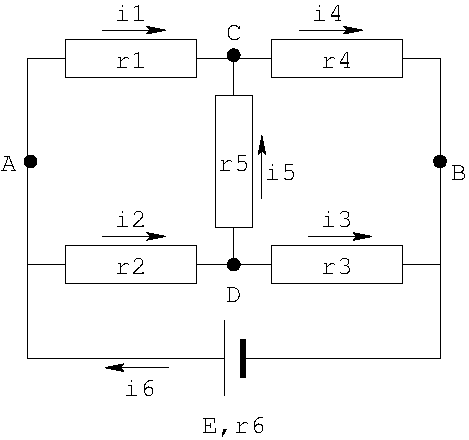
\includegraphics[width=6cm]{wheatstone.pdf}$$
$$
\begin{array}{lcr}
r_1 & = & 10 \Omega \\
r_2 & = & 10 \Omega \\
r_3 & = &  5 \Omega \\
r_4 & = & 20 \Omega \\
r_5 & = & 10 \Omega \\
r_6 & = & 10 \Omega \\
E   & = & 12 V 
\end{array}
\hspace*{5mm}
\left|\begin{array}{l}
i_4 = i_1 + i_5\\
i_6 = i_1 + i_2\\
i_2 = i_3 + i_5\\
10 i_1 = 10 i_2 + 10 i_5\\
10 i_5 = 5 i_3 - 20 i_4\\
12 - 10 i_6 = 10 i_2 + 5 i_3
\end{array}\right.
$$
\end{fig}

De nombreux exemples traités dans les enseignements scientifiques
conduisent à la nécessité de résoudre un système de $n$ équations linéaires
à $n$ inconnues, homogènes ou non homogènes, du type $A\cdot x = b$. 
La figure \ref{fig:wheatstone}
propose à titre d'exemple le cas du pont de Wheatstone en électricité.
Les ponts ont été utilisés pour la mesure des résistances, inductances et
capacités jusqu'à ce que les progrès en électronique les rendent obsolètes en
métrologie. Toutefois la structure en pont reste encore utilisée dans de 
nombreux montages.

La première méthode généralement utilisée pour trouver la solution 
d'un système d'équa\-tions linéaires tel que le système (\ref{eq1}) 
est celle qui consiste à éliminer les inconnues 
($x_i$) en combinant les équations.
Pour illustrer cette méthode, nous commencerons par étudier un exemple
simple pouvant s'effectuer {\em à la main}, 
puis nous passerons au cas général pour
présenter la méthode d'élimination de {\sc Gauss}.

%-------------------------------------------------------------------------
\subsection*{Etude d'un cas particulier}
\label{casparticulier}
%-------------------------------------------------------------------------
Considérons le système suivant :
$$\left\{
\begin{array}{rcrcrcr}
 x_0 & + &  x_1 & + &   x_2 & = &  1 \\
2x_0 & + & 4x_1 & + &  8x_2 & = & 10 \\
3x_0 & + & 9x_1 & + & 27x_2 & = & 33
\end{array}
\right.$$

Pour résoudre un tel système, l'idée de base est de triangulariser 
le système de telle manière qu'il soit possible de remonter les
solutions par substitutions successives.

La première étape consiste à éliminer le terme en $x_0$ des 
$2^{\grave eme}$ et $3^{\grave eme}$ équations.
Cherchons tout d'abord à éliminer le terme en $x_0$ de la $2^{\grave eme}$
équation. Pour cela nous multiplions la $1^{\grave ere}$ équation par le 
coefficient de $x_0$ de la $2^{\grave eme}$ équation ($a_{10} = 2$). 
On obtient le nouveau système :
$$\left\{
\begin{array}{rcrcrcr}
2x_0 & + & 2x_1 & + &  2x_2 & = &  2 \\
2x_0 & + & 4x_1 & + &  8x_2 & = & 10 \\
3x_0 & + & 9x_1 & + & 27x_2 & = & 33
\end{array}
\right.$$
On soustrait alors la première équation de la deuxième équation, 
ce qui conduit au système :
$$\left\{
\begin{array}{rcrcrcr}
2x_0 & + & 2x_1 & + &  2x_2 & = &  2 \\
     &   & 2x_1 & + &  6x_2 & = &  8 \\
3x_0 & + & 9x_1 & + & 27x_2 & = & 33
\end{array}
\right.$$
On recommence l'opération pour éliminer le terme en $x_0$ de la $3^{\grave eme}$
équation. Pour cela, on ramène à $1$ le coefficient de $x_0$ dans
la première équation en divisant cette équation par 2 ($a_{00} = 2$),
puis nous multiplions la $1^{\grave ere}$ équation par le 
coefficient de $x_0$ de la $3^{\grave eme}$ équation ($a_{20} = 3$). 
$$\left\{
\begin{array}{rcrcrcr}
3x_0 & + & 3x_1 & + &  3x_2 & = &  3 \\
     &   & 2x_1 & + &  6x_2 & = &  8 \\
3x_0 & + & 9x_1 & + & 27x_2 & = & 33
\end{array}
\right.$$
On soustrait ensuite la $1^{\grave ere}$ équation de la $3^{\grave eme}$ équation :
$$\left\{
\begin{array}{rcrcrcr}
3x_0 & + & 3x_1 & + &  3x_2 & = &  3 \\
     &   & 2x_1 & + &  6x_2 & = &  8 \\
     &   & 6x_1 & + & 24x_2 & = & 30
\end{array}
\right.$$
On obtient un nouveau système linéaire dans lequel seule la première équation contient
un terme en $x_0$.
L'équation utilisée (ici la $1^{\grave ere}$ équation) pour éliminer une inconnue 
dans les équations qui suivent (ici les $2^{\grave eme}$ et $3^{\grave eme}$ équations)
est appelée l'équation-pivot. Dans l'équation-pivot choisie, le coefficient de 
l'inconnue qui est éliminée dans les autres équations est appelé le pivot de
l'équation (ici $a_{00}$).

La deuxième étape consiste à éliminer le terme en $x_1$ de la troisième équation
en utilisant la deuxième équation comme équation-pivot. On ramène à $1$ le coefficient 
de $x_1$ dans la $2^{\grave eme}$ équation en divisant l'équation par 2 ($a_{11} = 2$),
puis on la multiplie par 6 ($a_{21} = 6$) pour que les $2^{\grave eme}$ et 
$3^{\grave eme}$ équations aient le même terme en $x_1$. Tout revient à
multiplier la $2^{\grave eme}$ équation par 3 ($a_{21}/a_{11} = 6/2 = 3$) :
$$\left\{
\begin{array}{rcrcrcr}
3x_0 & + & 3x_1 & + &  3x_2 & = &  3 \\
     &   & 6x_1 & + & 18x_2 & = & 24 \\
     &   & 6x_1 & + & 24x_2 & = & 30
\end{array}
\right.$$
Il reste à soustraire la $2^{\grave eme}$ équation de la $3^{\grave eme}$
pour éliminer le terme en $x_1$ de la $3^{\grave eme}$ équation :
$$\left\{
\begin{array}{rcrcrcr}
3x_0 & + & 3x_1 & + &  3x_2 & = &  3 \\
     &   & 6x_1 & + & 18x_2 & = & 24 \\
     &   &      &   &  6x_2 & = &  6
\end{array}
\right.$$
On obtient ainsi un système triangulaire d'équations linéaires 
dont on peut calculer
directement la valeur de $x_2$ par la $3^{\grave eme}$ équation : $6x_2 =  6 \Rightarrow
x_2 = 1$. On porte cette valeur de $x_2$ dans la deuxième équation, ce qui nous permet de
calculer $x_1$ : $6x_1 + 18\cdot 1 = 24 \Rightarrow x_1 = 1$. En reportant les valeurs de
$x_2$ et $x_1$ dans la première équation, on en déduit la valeur de $x_0$ :
$3x_0 + 3\cdot 1 +  3\cdot 1 =  3 \Rightarrow x_0 = -1$. 
On vérifie simplement que
les valeurs obtenues sont solutions du système initial :
$$\left\{
\begin{array}{rcrcrcr}
 x_0 & + &  x_1 & + &   x_2 & = &  1 \\
2x_0 & + & 4x_1 & + &  8x_2 & = & 10 \\
3x_0 & + & 9x_1 & + & 27x_2 & = & 33
\end{array}
\right.
\hspace*{2cm}
\left(
\begin{array}{rrr}
1 & 1 &  1 \\
2 & 4 &  8 \\
3 & 9 & 27 
\end{array}
\right)
\cdot
\left(
\begin{array}{r}
-1 \\ 1 \\ 1
\end{array}
\right)
=
\left(
\begin{array}{r}
1 \\ 10 \\ 33
\end{array}
\right)$$

%-------------------------------------------------------------------------
\subsection*{Etude du cas général}
\label{casgeneral}
%-------------------------------------------------------------------------
De manière générale, la méthode précédente consiste à réduire le système de $n$ 
équations à $n$ inconnues à un système triangulaire équivalent qui peut 
être ensuite résolu facilement par substitutions. En quelque sorte le système 
(\ref{eq1}) doit être transformé en un système équivalent du type :
\begin{equation}\label{eq2}
\left\{
\begin{array}{rcrcrcrcr@{\ =\ }r}
a_{00}x_0 &+& a_{01}x_1       &+& a_{02}x_2       &+& \cdots &+& a_{0(n-1)}x_{(n-1)}       & b_0\\
          & & a^{(1)}_{11}x_1 &+& a^{(1)}_{12}x_2 &+& \cdots &+& a^{(1)}_{1(n-1)}x_{(n-1)} & b^{(1)}_1\\
          & &                 &+& a^{(2)}_{22}x_2 &+& \cdots &+& a^{(2)}_{2(n-1)}x_{(n-1)} & b^{(2)}_2\\
          & &                 & &                 & & \cdots &+& \cdots           & \cdots\\
          & &                 & &                 & &        & & a^{(n-2)}_{(n-1)(n-1)}x_{(n-1)}   & b^{(n-2)}_{(n-1)}
\end{array}
\right.
\end{equation}
où l'indice supérieur désigne le nombre d'étapes à la suite desquelles est obtenu le 
coefficient considéré.

L'équation de rang 0 du système (\ref{eq1}) est d'abord divisée par le coefficient 
$a_{00}$ de $x_0$ (supposé non nul). On obtient :
\begin{equation}\label{eq3}
x_0 + \frac{a_{01}}{a_{00}}x_1 + \frac{a_{02}}{a_{00}}x_2 + \cdots + \frac{a_{0(n-1)}}{a_{00}}x_{(n-1)} = \frac{b_0}{a_{00}}
\end{equation}
Cette équation (\ref{eq3}) est alors multiplié par $a_{10}$, coefficient de $x_0$ dans 
la deuxième équation du système (\ref{eq1}). Le résultat est ensuite soustrait de la 
deuxième équation du système (\ref{eq1}), ce qui élimine $x_0$ dans la deuxième équation.
D'une manière générale on multiplie la relation (\ref{eq3}) par $a_{i0}$, coefficient
de $x_0$ dans l'équation de rang $i$ du système (\ref{eq1}) et on retranche le résultat
obtenu de cette même $i^{\grave eme}$ équation. A la fin $x_0$ est éliminé de toutes les équations, excepté de la première, et on obtient le système ainsi transformé :
\begin{equation}\label{eq4}
\left\{
\begin{array}{rcrcrcrcr@{\ =\ }r}
a_{00}x_0 &+& a_{01}x_1       &+& a_{02}x_2       &+& \cdots &+& a_{0(n-1)}x_{(n-1)}       & b_0\\
          & & a^{(1)}_{11}x_1 &+& a^{(1)}_{12}x_2 &+& \cdots &+& a^{(1)}_{1(n-1)}x_{(n-1)} & b^{(1)}_1\\
          & & a^{(1)}_{21}x_1 &+& a^{(1)}_{22}x_2 &+& \cdots &+& a^{(1)}_{2(n-1)}x_{(n-1)} & b^{(1)}_2\\
          & & a^{(1)}_{31}x_1 &+& a^{(1)}_{32}x_2 &+& \cdots &+& a^{(1)}_{3(n-1)}x_{(n-1)} & b^{(1)}_3\\
          & & \cdots          &+& \cdots          &+& \cdots &+& \cdots                    & \cdots\\
          & & a^{(1)}_{(n-1)1}x_1 &+& a^{(1)}_{(n-1)2}x_2 &+& \cdots &+& a^{(1)}_{(n-1)(n-1)}x_{(n-1)}   & b^{(1)}_{(n-1)}
\end{array}
\right.
\end{equation}
L'équation de rang 1 dans le nouveau système (\ref{eq4}) devient alors l'équation-pivot
et $a^{(1)}_{11}$ le pivot de l'équation. De la même façon on élimine $x_1$ des
équations du rang $2$ au rang $n-1$ dans le système (\ref{eq4}), et on obtient :
\begin{equation}\label{eq5}
\left\{
\begin{array}{rcrcrcrcr@{\ =\ }r}
a_{00}x_0 &+& a_{01}x_1       &+& a_{02}x_2       &+& \cdots &+& a_{0(n-1)}x_{(n-1)}       & b_0\\
          & & a^{(1)}_{11}x_1 &+& a^{(1)}_{12}x_2 &+& \cdots &+& a^{(1)}_{1(n-1)}x_{(n-1)} & b^{(1)}_1\\
          & &                 & & a^{(2)}_{22}x_2 &+& \cdots &+& a^{(2)}_{2(n-1)}x_{(n-1)} & b^{(2)}_2\\
          & &                 & & a^{(2)}_{32}x_2 &+& \cdots &+& a^{(2)}_{3(n-1)}x_{(n-1)} & b^{(2)}_3\\
          & &                 & & \cdots          &+& \cdots &+& \cdots                    & \cdots\\
          & &                 & & a^{(2)}_{(n-1)2}x_2 &+& \cdots &+& a^{(2)}_{(n-1)(n-1)}x_{(n-1)}   & b^{(2)}_{(n-1)}
\end{array}
\right.
\end{equation}
L'équation de rang 2 dans le nouveau système (\ref{eq5}) fait office à son tour d'équation
pivot, et ainsi de suite jusqu'à obtenir le système triangulaire (\ref{eq2}).
Une fois obtenu ce système triangulaire, on calcule directement
la valeur de $x_{(n-1)}$ par la dernière relation du système triangulaire. 
En portant cette valeur dans la relation précédente, on calculera
$x_{(n-2)}$, et ainsi de suite en remontant le système triangulaire (\ref{eq2}).
A chaque étape $k$, on a donc les relations suivantes :
\begin{enumerate}
\item {Triangularisation}
	$$\left\{
	\begin{array}{lcl}
	a_{ij}^{(k)} & = & \displaystyle a_{ij}^{(k-1)} - \frac{a_{ip}^{(k-1)}}{a_{pp}^{(k-1)}}\cdot
	a_{pj}^{(k-1)} \\[5mm]
	b_i^{(k)}    & = & \displaystyle b_i^{(k-1)} - \frac{a_{ip}^{(k-1)}}{a_{pp}^{(k-1)}}\cdot
	b_p^{(k-1)}
	\end{array}
	\right.\mbox{\footnotesize\ avec\ }
	\left\{
	\begin{array}{l}
	k\ :\ \mbox{\footnotesize étape}\\
	p\ : \ \mbox{\footnotesize rang du pivot}\\[5mm]
	p < i \leq (n-1) \\[2mm]
	p \leq j \leq (n-1)
	\end{array}
	\right.$$
\item {Remontée par substitutions} 
	$$\left\{
	\begin{array}{lcl}
	x_{(n-1)} & = & \displaystyle\frac{b_{(n-1)}}{a_{(n-1)(n-1)}}\\[5mm]
	x_i       & = & \displaystyle\frac{\displaystyle b_{i} - 
	\sum_{j=i+1}^{n-1} a_{ij}x_j}{a_{ii}} 
	\end{array}
	\right.
	\mbox{\ avec\ } 0 \leq i < (n-1)$$
\end{enumerate}

Jusqu'à présent, on a admis que le pivot au cours du processus de triangularisation 
était non nul ($a_{pp} \neq 0$). Si ce n'est pas le cas, on doit permuter 
l'équation-pivot avec une autre ligne dans laquelle le pivot est différent de 0.
Il se peut également que le pivot, sans être nul, soit très petit et l'on a 
intérêt là-aussi à interchanger les lignes comme pour le cas d'un pivot nul.
En fait, pour augmenter la précision de la solution obtenue, on a toujours 
intérêt à utiliser la ligne qui a le plus grand pivot.

Cette méthode est connue sous le nom de méthode d'élimination 
de {\sc Gauss} (également connue sous
le nom de méthode de triangularisation de {\sc Gauss} ou méthode du pivot 
de {\sc Gauss}). Elle fut nommée ainsi en l'honneur du mathématicien allemand 
{\sc Johann Carl Friedrich Gauss} (1777--1855), mais elle est connue des Chinois 
depuis au moins le $1^{er}$ siècle de notre ère. Elle est référencée dans le livre 
chinois « Jiuzhang suanshu~» où elle est attribuée à {\sc Chang Ts'ang} chancelier de 
l'empereur de Chine au $2^{\grave eme}$ siècle avant notre ère. 


%-------------------------------------------------------------------------
\subsection*{Jeu de tests}
%-------------------------------------------------------------------------
L'algorithme de résolution de tels systèmes linéaires pourra être testé
à l'aide des systèmes suivants :
$$\begin{array}{|l|c|c|c|}
\hline
\mbox{\bf Test} & \multicolumn{2}{|c|}{\mbox{{\bf Système} $A\cdot x = b$}} & \bf Solution\\
\cline{2-3}
                & A & b & \bf exacte \\
\hline
\hline
1 
& 
\left(\begin{array}{r}
4
\end{array}\right) 
&
\left(\begin{array}{r}
1
\end{array}\right) 
&
\displaystyle
\left(\begin{array}{r}
1/4
\end{array}\right)\\
\hline
2 
& 
\left(\begin{array}{rr}
1 & 1 \\
1 & -1
\end{array}\right) 
&
\left(\begin{array}{r}
1 \\ 0
\end{array}\right)
&
\displaystyle
\left(\begin{array}{r}
1/2 \\ 1/2
\end{array}\right)
\\
\hline
3 
& 
\left(\begin{array}{rrr}
2 & -1 & 2 \\
1 & 10 & -3 \\
-1 & 2 & 1
\end{array}\right) 
&
\left(\begin{array}{r}
2 \\ 5 \\ -3
\end{array}\right)
&
\left(\begin{array}{r}
2 \\ 0 \\ -1
\end{array}\right)
\\
\hline
\end{array}$$


$$\begin{array}{|l|c|c|c|}
\hline
\mbox{\bf Test} & \multicolumn{2}{|c|}{\mbox{{\bf Système} $A\cdot x = b$}} & \bf Solution\\
\cline{2-3}
                & A & b & \bf exacte \\
\hline
4 &
\left(\begin{array}{rrrr}
10 & 7 & 8 & 7 \\
7 & 5 & 6 & 5 \\
8 & 6 & 10 & 9 \\
7 & 5 & 9 & 10
\end{array}\right) 
&
\left(\begin{array}{r}
32 \\ 23 \\ 33 \\ 31
\end{array}\right) 
&
\left(\begin{array}{r}
1 \\ 1 \\ 1 \\ 1
\end{array}\right) 
\\
\hline
5 & 
\left(\begin{array}{rrrr}
10 & 7 & 8.1 & 7.2 \\
7.08 & 5.04 & 6 & 5 \\
8 & 5.98 & 9.89 & 9 \\
6.99 & 4.99 & 9 & 9.98
\end{array}\right) 
&
\left(\begin{array}{r}
32 \\ 23 \\ 33 \\ 31
\end{array}\right) 
&
\mbox{---} \\
\hline
6 &
\left(\begin{array}{rrrr}
10 & 7 & 8 & 7 \\
7 & 5 & 6 & 5 \\
8 & 6 & 10 & 9 \\
7 & 5 & 9 & 10
\end{array}\right) 
&
\left(\begin{array}{r}
32.01 \\ 22.99 \\ 33.01 \\ 30.99
\end{array}\right) 
&
\mbox{---} \\
\hline
\end{array}$$

Les tests 5 et 6 sont des variations du test 4 : $A_5 = A_4 + \Delta A$
et $b_6 = b_4 + \Delta b$. Ces 2 tests sont effectués pour évaluer 
les conséquences sur la solution $x$ d'une perturbation $\Delta A$ de $A_4$
et d'une perturbation $\Delta b$ de $b_4$.
$$\Delta A = \left(\begin{array}{rrrr}
0 & 0 & 0.1 & 0.2\\
0.08 & 0.04 & 0 & 0\\
0 & -0.02 & -0.11 & 0\\
-0.01 & -0.01 & 0 & -0.02
\end{array}
\right)$$
$$\Delta b = \left(\begin{array}{r}
0.01 \\ - 0.01 \\ 0.01 \\ -0.01
\end{array}\right)$$
$$\begin{array}{|l|c|c|}
\hline
\mbox{\bf Test} & \multicolumn{2}{|c|}{\mbox{{\bf Système} $A\cdot x = b$}}\\
\cline{2-3}
                & A & b  \\
\hline
\hline
7 &
\left(\begin{array}{rrrrrr}
1 & 0 & 0 & - & 1 & 0\\
1 & 1 & 0 & 0 & 0 & -1\\
0 & 1 & -1 & 0 & -1 & 0\\
10 & -10 & 0 & 0 & -10 & 0\\
0 & 0 & 5 & -20 & -10 & 0\\
0 & 10 & 5 & 0 & 0 & 10
\end{array}\right) 
&
\left(\begin{array}{r}
0 \\ 0 \\ 0 \\ 0 \\ 0 \\ 12
\end{array}\right)\\
\hline
8 &
\left(\begin{array}{rrrrrrrr}
1 & 0 & 0 & 0 & 0 & 0 & 0 & 0\\
1 & 2\pi & 4\pi^2 & 8\pi^3 & 16\pi^4 & 32\pi^5 & 64\pi^6 & 128\pi^7\\
0 & 1 & 0 & 0 & 0 & 0 & 0 & 0\\
0 & 1 & 4\pi & 12\pi^2 & 32\pi^3 & 80\pi^4 & 192\pi^5 & 448\pi^6\\
1 & \pi/2 & \pi^2/4 & \pi^3/8 & \pi^4/16 & \pi^5/32 & \pi^6/64 & \pi^7/128\\
0 & \pi/2 & \pi & 3\pi^2/4 & \pi^3/2 & 5\pi^4/16 & 3\pi^5/16 & 7\pi^6/64\\
1 & \pi & \pi^2 & \pi^3 & \pi^4 & \pi^5 & \pi^6 & \pi^7\\
0 & \pi & 2\pi & 3\pi^2 & 4\pi^3 & 5\pi^4 & 6\pi^5 & 7\pi^6
\end{array}\right) 
&
\left(\begin{array}{r}
4 \\ 4 \\ 0 \\ 0 \\ 2 \\ -2 \\ 1 \\ 0
\end{array}\right)\\
\hline
\end{array}$$


Le test 7 correspond à l'exemple du pont de Wheatstone 
(figure \ref{fig:wheatstone}). Le test 8 correspond
à la détermination de la forme d'une came rotative qui doit
mettre en mouvement un axe suivant une loi horaire donnée.

%-------------------------------------------------------------------------

%-------------------------------------------------------------------------
\chapter*{Liste des exercices}
\addcontentsline{toc}{chapter}{Liste des exercices}
	\listtheorems{td}
%-------------------------------------------------------------------------


\label{fin}
%-------------------------------------------------------------------------
\end{document}
%-------------------------------------------------------------------------
